% concatenated from Discrete_homotopy_groups_of_cubical_sets.tex
\documentclass[oneside, 12pt]{amsart}

\usepackage{amsmath, amssymb, amsthm, amsfonts}
%\usepackage{here}
\usepackage{newtxtext,newtxmath}
%\usepackage{mathabx}
%\usepackage{microtype}
%\usepackage{lmodern}
\usepackage[cal=euler,scr=rsfs]{mathalfa}
\usepackage[all]{xy}
%\usepackage[dvipdfmx]{graphicx}
\usepackage[a4paper, margin=1.1in]{geometry}
\usepackage{tikz}
\usetikzlibrary{arrows.meta}
\usetikzlibrary{decorations.markings}
\usepackage[backref=page]{hyperref}
\hypersetup{pdfborder={0 0 0}, colorlinks=true, urlcolor=blue, linkcolor=blue, citecolor=red}
%\usepackage{showkeys}
%\usepackage{setspace}
%\setstretch{1.05}

% equation numbers
\numberwithin{equation}{section}

% xypic arrow shape
\SelectTips{eu}{12}

% tikz arrow
\tikzset{myarrow/.style={postaction={decorate},decoration={markings,mark=at position #1 with {\arrow{latex}},}}}

% enumeration number fonts
%\renewcommand{\theenumi}{\roman{enumi}}

% theorem environments
\theoremstyle{plain}
\newtheorem{theorem}{Theorem}[section]
\newtheorem{proposition}[theorem]{Proposition}
\newtheorem{lemma}[theorem]{Lemma}
\newtheorem{corollary}[theorem]{Corollary}
\newtheorem{conjecture}[theorem]{Conjecture}
\newtheorem{problem}[theorem]{Problem}
\newtheorem{question}[theorem]{Question}

\theoremstyle{definition}
\newtheorem{definition}[theorem]{Definition}
\newtheorem{example}[theorem]{Example}
\newtheorem{assumption}[theorem]{Assumption}

\theoremstyle{remark}
\newtheorem{remark}[theorem]{Remark}

% commands
\newcommand{\N}{\mathbb{N}}
\newcommand{\Z}{\mathbb{Z}}
\newcommand{\Q}{\mathbb{Q}}
\newcommand{\R}{\mathbb{R}}
\newcommand{\C}{\mathbb{C}}
\newcommand{\cSet}{\mathsf{cSet}}
\newcommand{\SymcSet}{\mathsf{SymcSet}}
\newcommand{\QSymcSet}{\mathsf{QSymcSet}}
\newcommand{\sd}{\operatorname{sd}}
\newcommand{\ex}{\operatorname{Ex}}

%\newcommand{\kishimoto}[1]{\noindent{\color{blue}\textbf{Kishimoto: #1}}}
%\newcommand{\tong}[1]{\noindent{\color{red}\textbf{Tong: #1}}}



% title
\title{Discrete homotopy groups of cubical sets}

\author{Daisuke Kishimoto}
\address{Faculty of Mathematics, Kyushu University, Fukuoka 819-0395, Japan}
\email{kishimoto@math.kyushu-u.ac.jp}

\author{Yichen Tong}
\address{Institute for Theoretical Sciences, Westlake Institute of Advanced Study, Westlake University, Hangzhou 310030, China}
\email{tongyichen@westlake.edu.cn}

\date{\today}

\subjclass[2020]{55Q05, 55U35, 18N40, 05C20}

\keywords{cubical set, symmetric cubical set, quasisymmetric cubical set, discrete homotopy group, Hurewicz theorem, directed graph}



\begin{document}
	
	
	
	\begin{abstract}
		We extend the notion of discrete homotopy groups of graphs to arbitrary cubical sets, and show that the discrete homotopy groups of quasisymmetric cubical sets are naturally isomorphic to the homotopy groups of their geometric realizations. Here, quasisymmetric cubical sets are cubical sets equipped with coordinate permutation symmetries that are compatible with faces and degeneracies, but not necessarily with connections. We give a purely combinatorial construction of the left adjoint of the forgetful functor from the category of quasisymmetric cubical sets to the category of cubical sets, and prove that the unit of this adjunction is an objectwise weak equivalence. As a consequence, we obtain a purely combinatorial description of the homotopy groups of the geometric realizations of arbitrary cubical sets. As an application, we establish the Hurewicz theorem for the discrete homotopy groups of quasisymmetric cubical sets.
	\end{abstract}
	\maketitle
	\section{Introduction}\label{Introduction}
	
	Discrete homotopy theory, introduced in \cite{BBdLL,BKLW}, is a combinatorial homotopy theory of graphs. It builds on earlier work of Atkin \cite{At1,At2} concerning algebraic representations of simplicial complexes, and later reformulated in \cite{BL} as a homotopy theory of graphs and simplicial complexes. This theory has found numerous applications, including in matroid theory, hyperplane arrangements, combinatorial time series analysis and topological data analysis. The fundamental invariants in discrete homotopy theory of graphs are the $A$-groups, named after Atkins, which we refer to as the \emph{discrete homotopy groups}.
	
	
	
	Cubical sets form a classical combinatorial model for the homotopy theory of spaces. A cubical set is a presheaf on the category $\Box$ of combinatorial cubes, whereas a simplicial set is a presheaf on the category $\Delta$ of combinatorial simplices. Cubical sets arise naturally in the study of discrete homotopy theory of graphs. Babson, Barcelo, de Longueville, and Laubenbacher \cite{BBdLL} associated a space $X_G$ to a graph $G$, and conjectured that the homotopy groups of $X_G$ are isomorphic to the discrete homotopy groups of $G$. Carranza and Kapulkin \cite{CK2} later constructed a cubical set $\mathrm{N}_1G$, called the \emph{$1$-nerve} of $G$, whose geometric realization coincides with the space $X_G$. They showed that the homotopy groups of the geometric realization of $\mathrm{N}_1G$ are naturally isomorphic to the discrete homotopy groups of $G$, thereby proving the conjecture. Their proof relies on applying an appropriate fibrant replacement to the cubical set $\mathrm{N}_1G$.
	
	
	
	The discrete homotopy groups of a graph $G$ admit an interpretation in terms of cubes in the cubical set $\mathrm{N}_1G$. It is therefore natural to expect that discrete homotopy theory can be extended from graphs to cubical sets, with the discrete homotopy theory of graphs embedded via the $1$-nerve construction. In this paper, we extend the notion of discrete homotopy groups of graphs to arbitrary cubical sets in a purely combinatorial manner, in contrast to the definition of the homotopy groups of cubical Kan complexes \cite{CK1}. Carranza and Kapulkin \cite{CK1} defined homotopy equivalences of cubical sets in close analogy with homotopy equivalences of topological spaces, and the discrete homotopy groups of cubical sets are invariant under homotopy equivalences.
	
	
	
	Every $n$-cube is the product of $n$ copies of the $1$-cube, and thus every cube carries an intrinsic symmetry arising from permutations of its coordinates. This symmetry is implicitly and frequently used in classical homotopy theory, for example in the Eckmann-Hilton argument. However, the category $\Box$ itself is not endowed with this symmetry. We define a \emph{quasisymmetric cubical set} by adjoining coordinate permutation symmetries that are required to be compatible with faces and degeneracies, but not necessarily with connections. Grandis and Mauri \cite{GM1} introduced a category obtained from $\Box$ by adjoining the coordinate permutation symmetries that are compatible with faces, degeneracies, and connections. Later, Isaacson \cite{I} introduced the term \emph{symmetric cubical set} for a presheaf on this category and studied the category of symmetric cubical sets from the perspective of model category theory. In particular, he showed that symmetric cubical sets also form a model for the homotopy theory of spaces. By definition, the class of quasisymmetric cubical sets strictly contains that of symmetric cubical sets.
	
	
	
	For a cubical set $X$, let $|X|$ denote its geometric realization. For a pointed cubical set $(X,x_0)$, let $\pi_n^\delta(X,x_0)$ denote its $n$-th discrete homotopy group. Our first main result is the following. As a consequence, we obtain a combinatorial description of the homotopy groups of the geometric realization of an arbitrary quasisymmetric cubical set, which is not necessarily a Kan complex.
	
	
	
	\begin{theorem}
		\label{main 1}
		Let $(X,x_0)$ be a pointed quasisymmetric cubical set. There is a natural isomorphism
		\[
		\pi_*^\delta(X,x_0)\cong\pi_*(|X|,x_0).
		\]
	\end{theorem}
%	\tong{Let $(X,x_0)$ be a pointed cubical set which is pointed homotopy equivalent to a pointed quasisymmetric cubical set. Then there is a natural isomorphism
%		\[
%		\pi_*^\delta(X,x_0)\cong\pi_*(|X|,x_0).
%		\]
%	}
	
	
	Let $\cSet$ and $\SymcSet$ denote the categories of cubical sets and symmetric cubical sets. In \cite{I}, Isaacson showed that the forgetful functor $\mathcal{U}\colon\SymcSet\to\cSet$ admits a left adjoint $\mathcal{F}\colon\cSet\to\SymcSet$ such that the unit $1_\cSet\Rightarrow\mathcal{UF}$ is an objectwise weak equivalence, where a weak equivalence is a cubical map that induces isomorphisms on homotopy groups of geometric realizations with respect to all basepoints. The left adjoint $\mathcal{F}$ is defined via a left Kan extension, and is therefore not explicit. Let $\QSymcSet$ denote the category of quasisymmetric cubical sets. In this paper, we combinatorially and explicitly construct the left adjoint of the forgetful functor $\mathcal{U}\colon\QSymcSet\to\cSet$, and prove the following second main result. As a consequence, we obtain a combinatorial description of the homotopy groups of the geometric realization of an arbitrary cubical set.
	
	
	
	\begin{theorem}
		\label{main 2}
		One can combinatorially construct the left adjoint $\mathcal{S}\colon\cSet\to\QSymcSet$ of the forgetful functor $\mathcal{U}\colon\QSymcSet\to\cSet$ such that the unit
		\[
		1_{\cSet}\Rightarrow\mathcal{U}\mathcal{S}
		\]
		is an objectwise weak equivalence.
	\end{theorem}
%	Combining Theorem \ref{main 2} with the constructions of Section \ref{Fibrant replacement}, we obtain a functor
%	\[
%	\mathcal{G}_0\mathcal{RUS}\colon \cSet \to \cSet
%	\]
%	together with a natural weak equivalence
%	\[
%	1_{\cSet}\Rightarrow \mathcal{G}_0\mathcal{RUS},
%	\]
%	such that \(\mathcal{G}_0\mathcal{RUS}\) sends every cubical set to a quasisymmetric Kan complex. Consequently, for any pointed Kan complex \((X,x_0)\) which is not necessarily quasisymmetric, this fibrant replacement, together with the homotopy invariance of the discrete homotopy groups, yields a natural isomorphism
%	\[
%	\pi_*(X,x_0)\cong \pi_*^\delta(X,x_0).
%	\]
	
	Combining Theorem \ref{main 2} with the constructions of Section \ref{Fibrant replacement}, we obtain a functorial fibrant replacement which sends a cubical set to a quasisymmetric Kan complex. Consequently, for any pointed Kan complex \((X,x_0)\) which is not necessarily quasisymmetric, this fibrant replacement, together with the homotopy invariance of the discrete homotopy groups, yields a natural isomorphism
	\[
	\pi_*(X,x_0)\cong \pi_*^\delta(X,x_0).
	\]
	Note that the discrete homotopy groups on the right-hand side are defined purely combinatorially, whereas the homotopy groups on the left-hand side are defined homotopically. Finally, we apply Theorem \ref{main 1} to establish the Hurewicz theorem for the discrete homotopy groups of quasisymmetric cubical sets. The precise definition of the Hurewicz map will be given in Section \ref{Discrete homotopy groups of quasisymmetric cubical sets}. A cubical set $X$ is called \emph{$n$-connected} if $\pi_*^\delta(X,x_0)=0$ for all $*\le n$ and for every basepoint $x_0$.
	
	
	
	\begin{theorem}
		\label{main 3}
		Let $(X,x_0)$ be a pointed quasisymmetric cubical set. If $X$ is $(n-1)$-connected, then the map
		\[
		\pi_n^\delta(X,x_0)\to H_n(X),\quad[(x,s)]\mapsto\left[\sum_{i_1,\ldots,i_n}\mathrm{sgn}_{i_1,\ldots,i_n}(x)x(i_1,\ldots,i_n)\right]
		\]
		is the abelianization for $n=1$ and an isomorphism for $n\ge 2$.
	\end{theorem}

	
	The discrete homotopy theory of directed graphs has seen rapid development in recent years. This theory not only generalizes the homotopy theory of graphs but also captures the inherently directed nature of directed graphs. Grigor'yan, Lin, Muranov, and Yau \cite{GLMY2} introduced the path homology $\mathrm{PH}_*(G)$ in \cite{GLMY1} and the fundamental group $\pi_1(G,v)$ of a pointed directed graph $(G,v)$ in \cite{GLMY2}. They also proved a Hurewicz theorem for $\pi_1(G,v)$ in \cite{GLMY2}, with target the first path homology, and this one-dimensional Hurewicz theorem was subsequently generalized to a more elaborate version in \cite{KT} by the authors. 
	
	
	
	
	Later, Li, Wu, Yau, and Zhang introduced the higher homotopy group $\bar{\pi}_n(G,v)$ of a pointed directed graph in \cite{LWYZ}, which satisfies
	\[
	\bar{\pi}_1(G,v)\cong\pi_1(G,v).
	\] 
	Recently, Theriault, Wu, Yau, and Zhang constructed some directed graphs with nontrivial higher homotopy groups in \cite{TWYZ}. They used a homomorphism $\tilde{h}_*$ towards the path homology, which factors as
	\begin{equation}
		\label{TWYZ Hurewicz map}
		\bar{\pi}_n(G,v)\xrightarrow{h_*}\mathrm{QH}_n(G)\xrightarrow{\phi_G}\mathrm{PH}_n(G)
	\end{equation}
	Here $\mathrm{QH}_n(G)$ denotes the singular cubical homology group of $G$, a distinct homology theory developed in \cite{GM2}. We introduce the 1-nerve $\mathrm{N}_1G$ of a directed graph $G$, analogous to the 1-nerve of a graph, which is automatically a symmetric cubical set. By identifying the homomorphism $h_*\colon\bar{\pi}_n(G,v)\to \mathrm{QH}_n(G)$ with the discrete Hurewicz map $h_*\colon\pi_n^\delta(\mathrm{N}_1G,v)\to H_n(\mathrm{N}_1G)$, we establish the following result by applying Theorem \ref{main 3} to $\mathrm{N}_1G$. We say $G$ is $n$-connected if $\mathrm{N}_1G$ is $n$-connected. 
	\begin{theorem}
		\label{main 4}
		Let $(G,v)$ be a pointed directed graph. If $G$ is $(n-1)$-connected, then the homomorphism
		\[
		h_*\colon\bar{\pi}_n(G,v)\to \mathrm{QH}_n(G)
		\]
		is the abelianization for $n=1$ and an isomorphism for $n\ge2$.
	\end{theorem}
	Since the first path homology group and the first singular cubical homology group of a directed graph are isomorphic, our Hurewicz theorem generalizes the one in \cite{GLMY2}. We also provide an alternative proof of the Hurewicz theorem for graphs, which was originally proved in \cite{CK2}.

	
	The organization of this paper is as follows. In Section \ref{Preliminaries}, we recall some basic notions about cubical sets, including their definition, products, geometric realizations, and homotopy and homology groups. In Section \ref{Discrete homotopy groups of cubical sets}, we define the discrete homotopy groups for general cubical sets and discuss their properties. In Section \ref{Quasisymmetric cubical sets}, we recall the (signed) symmetric cubical category and the category of (signed) symmetric cubical sets, and then generalize them to the (signed) quasisymmetric cubical category and the category of (signed) quasisymmetric cubical sets. We also prove Theorem \ref{main 2} in this section. In Section \ref{Fibrant replacement}, we construct an explicit fibrant replacement of a quasisymmetric cubical set. We also compare our constructions with the classical \(\ex^\infty\) functor in simplicial homotopy theory by introducing a naive cubical analogue. In Section \ref{Discrete homotopy groups of quasisymmetric cubical sets}, we prove Theorems \ref{main 1} and \ref{main 3} using the fibrant replacement constructed in Section \ref{Fibrant replacement}. Finally, in Section \ref{Discrete homotopy groups of directed graphs}, we define the 1-nerve of a directed graph and prove Theorem \ref{main 4} by applying Theorem \ref{main 3} to this 1-nerve.
	
	\section*{Acknowledgment}
	The authors would like to thank Kensuke Arakawa for bringing relevant references to their attention, and Xing Gu for inspiring discussions. The first author was partially supported by JSPS KAKENHI Grant Numbers JP22K03284.
	
	\section{Preliminaries}\label{Preliminaries}
	
	In this section, we recall the basic notions of cubical sets and Kan complexes, together with several key constructions, including products and geometric realization. We also review the homology of cubical sets and the homotopy groups of Kan complexes.
	
	
	
	\subsection{Cubical sets}
	
	We begin by defining the cubical category $\Box$. Let $[1]$ denote the poset $\{0<1\}$. The \emph{cubical category} $\Box$ has objects $[1]^n$ for $n\ge 0$, and morphisms generated under composition by the following three classes of maps:
	
	\begin{itemize}
		\item (faces) $\partial_{i,\alpha}\colon[1]^{n-1}\to[1]^n$ for $i=1,\ldots,n$ and $\alpha=0,1$ given by
		\[
		\partial_{i,\alpha}(x_1,\ldots,x_{n-1})=(x_1,\ldots,x_{i-1},\alpha,x_i,\ldots,x_{n-1}).
		\]
		
		\item (degeneracies) $\sigma_i\colon[1]^n\to[1]^{n-1}$ for $i=1,\ldots,n$ given by
		\[
		\sigma_i(x_1,\ldots,x_n)=(x_1,\ldots,x_{i-1},x_{i+1},\ldots,x_n).
		\]
		
		\item (connections) $\gamma_{i,\alpha}\colon[1]^{n}\to[1]^{n-1}$ for $i=1,\ldots,n-1$ and $\alpha=0,1$ given by
		\begin{align*}
			\gamma_{i,0}(x_1,\ldots,x_{n})=(x_1,\ldots,x_{i-1},\max\{x_i,x_{i+1}\},x_{i+2},\ldots,x_n)\\
			\gamma_{i,1}(x_1,\ldots,x_{n})=(x_1,\ldots,x_{i-1},\min\{x_i,x_{i+1}\},x_{i+2},\ldots,x_n).
		\end{align*}
	\end{itemize}
	
	\noindent It is straightforward to verify that these maps satisfy the following \emph{cubical identities}:
	\begin{alignat*}{2}
		\partial_{j,\beta}\partial_{i,\alpha}&=\partial_{i+1,\alpha}\partial_{j,\beta}\quad(j\le i)&\sigma_i\sigma_j&=\sigma_j\sigma_{i+1}\quad(j\le i)\\
		\sigma_j\partial_{i,\alpha}&=
		\begin{cases}
			\partial_{i-1,\alpha}\sigma_j&(j<i)\\
			1&(j=i)\\
			\partial_{i,\alpha}\sigma_{j-1}&(j>i)
		\end{cases}&
		\gamma_{j,\beta}\gamma_{i,\alpha}&=
		\begin{cases}
			\gamma_{i,\alpha}\gamma_{j+1,\beta}&(j>i)\\
			\gamma_{i,\alpha}\gamma_{i+1,\alpha}&(j=i,\,\beta=\alpha)
		\end{cases}\\
		\gamma_{j,\beta}\partial_{i,\alpha}&=
		\begin{cases}
			\partial_{i-1,\alpha}\gamma_{j,\beta}&(j<i-1)\\
			1&(j=i-1,i,\,\beta=\alpha)\\
			\partial_{j,\alpha}\sigma_j&(j=i-1,i,\,\beta=1-\alpha)\\
			\partial_{i,\alpha}\gamma_{j-1,\beta}&(j>i)
		\end{cases}\;&
		\sigma_j\gamma_{i,\alpha}&=
		\begin{cases}
			\gamma_{i-1,\alpha}\sigma_j&(j<i)\\
			\sigma_i\sigma_i&(j=i)\\
			\gamma_{i,\alpha}\sigma_{j+1}&(j>i)
		\end{cases}
	\end{alignat*}
	One may regard the cubical category $\Box$ as the category whose objects are $[1]^n$ for $n\ge 0$ and whose morphisms are freely generated by faces, degeneracies and connections, subject to the cubical identities.
	
	
	
	As in the simplicial setting, morphisms in the cubical category admit standard factorizations; see \cite[Theorem 5.1]{GM1}.
	
	
	
	\begin{lemma}
		\label{factorization}
		Every morphism $f\colon[1]^m\to[1]^n$ in the cubical category $\Box$ admits a unique factorization
		\[
		f=(\partial_{i_1,\alpha_1}\cdots\partial_{i_r,\alpha_r})(\gamma_{j_1,\beta_1}\cdots\gamma_{j_s,\beta_s})(\sigma_{k_1}\cdots\sigma_{k_t}),
		\]
		where $i_1>\cdots>i_r$, $j_1\le\cdots\le j_s$ and $k_1<\cdots<k_t$ such that $\beta_p\ne\beta_{p+1}$ whenever $j_p=j_{p+1}$.
	\end{lemma}
	
	
	
	\begin{definition}
		The category $\cSet$ is the functor category $\mathsf{Set}^{\Box^\mathrm{op}}$. The objects and morphisms of $\cSet$ are referred to as \emph{cubical sets} and \emph{cubical maps}.
	\end{definition}
	
	
	
	\begin{remark}
		In this paper we work with cubical sets equipped with \emph{connections}. Connections on cubical sets were introduced by Brown and Higgins \cite{BH} as additional degeneracies. Although connections are not always assumed in the literature, they play a crucial role in the homotopy theory of cubical sets and will be essential for our purposes.
	\end{remark}
	
	
	
	
	Let $X$ be a cubical set. For $n\ge 0$, we write $X_n=X([1]^n)$, and denote by $X$ the union of the sets $X_n$ over all $n\ge 0$, when no confusion is likely to arise. As in the simplicial setting, every cubical set is equivalently described by a collection of sets $\{X_n\}_{n\ge 0}$ together with faces, degeneracies, and connections satisfying the cubical identities. An element of $X_n$ is called an \emph{$n$-cube}. We introduce three basic examples of cubical sets.
	
	
	
	\begin{example}
		\begin{enumerate}
			\item The cubical set $\Box^n=\Box(-,[1]^n)$ is called the \emph{$n$-cube}.
			
			\item The \emph{boundary} of $\Box^n$ is the cubical subset
			\[
			\partial\Box^n=\bigcup_{\substack{i=1,\ldots,n\\\alpha=0,1}}\mathrm{Im}\,\partial_{i,\alpha}.
			\]
			
			\item For $i=1,\ldots,n$ and $\alpha=0,1$, the \emph{$(i,\alpha)$-horn} in $\Box^n$ is the cubical subset of $\partial\Box^n$ defined by
			\[
			\sqcap^n_{i,\alpha}=\bigcup_{(j,\beta)\ne(i,\alpha)}\mathrm{Im}\,\partial_{j,\beta}.
			\]
		\end{enumerate}
	\end{example}
	
	
	
	Let $X$ be a cubical set. By definition, there is a one-to-one correspondence between $X_n$ and the set of cubical maps $\Box^n\to X$. This justifies the terminology: both $\Box^n$ and the elements of $X_n$ are called $n$-cubes. Given a morphism $\theta$ in $\Box$ and an element $x\in X$, we may regard the cube obtained by applying $\theta$ to $x$ as the composite
	\[
	\Box^m\xrightarrow{\theta}\Box^n\xrightarrow{x}X.
	\]
	Hence we denote it by $x\theta$. An $n$-cube $x\in X_n$ is called \emph{degenerate} if there exist $i\in\{1,\ldots,n\}$ and an element $y\in X_{n-1}$ such that $x=y\sigma_i$. Otherwise, $x$ is called \emph{nondegenerate}.
	
	
	
	\begin{definition}
		A cubical set $X$ is called a \emph{Kan complex} if for any $n\ge 1$, $i=1,\ldots,n$ and $\alpha=0,1$, every cubical map $\sqcap_{i,\alpha}^n\to X$ extends to a cubical map $\Box^n\to X$.
	\end{definition}
	
	
	
	\begin{example}
		Define the singular functor $\mathrm{Sing}\colon\mathsf{Top}\to\cSet$ by setting $(\mathrm{Sing}\,X)_n$ to be the set of continuous maps $[0,1]^n\to X$, where faces, degeneracies and connections are induced from the corresponding maps between cubes. Then for every space $X$, the cubical set $\mathrm{Sing}\,X$ is a Kan complex.
	\end{example}
	
	
	
	\subsection{Products}
	
	We define a product of cubical sets.
	
	\begin{definition}
		The functor
		\[
		\otimes\colon\cSet\times\cSet\to\cSet
		\]
		is defined as follows. For cubical sets $X$ and $Y$, the cubical set $X\otimes Y$ is given in degree $n$ by
		\[
		(X\otimes Y)_n=\left(\coprod_{k+l=n}X_k\times Y_l\right)/(x\sigma_{k+1},y)\sim(x,y\sigma_1)
		\]
		Faces, degeneracies and connections are defined by
		\begin{align*}
			(x,y)\partial_{i,\alpha}&=
			\begin{cases}
				(x\partial_{i,\alpha},y)&(i=1,\ldots,k)\\
				(x,y\partial_{i-k,\alpha})&(i=k+1,\ldots,k+l)
			\end{cases}\\
			(x,y)\sigma_i&=
			\begin{cases}
				(x\sigma_i,y)&(i=1,\ldots,k+1)\\
				(x,y\sigma_{i-k})&(i=k+1,\ldots,k+l)
			\end{cases}\\
			(x,y)\gamma_{i,\alpha}&=
			\begin{cases}
				(x\gamma_{i,\alpha},y)&(i=1,\ldots,k)\\
				(x,y\gamma_{i-k,\alpha})&(i=k+1,\ldots,k+l)
			\end{cases}
		\end{align*}
		where $(x,y)\in X_k\times Y_l$.
	\end{definition}
	
	
	
	\begin{example}
		It is straightforward to verify that there is a natural isomorphism
		\[
		\Box^m\otimes\Box^n\cong\Box^{m+n}.
		\]
	\end{example}
	
	
	
	By definition, the functor $\otimes\colon\cSet\times\cSet\to\cSet$ is a monoidal product. Define a functor $\otimes\colon\Box\times\Box\to\Box$ by $\otimes([1]^m,[1]^n)=[1]^{m+n}$. By \cite[Proposition 1.24]{DKLS}, the functor $\otimes\colon\cSet\times\cSet\to\cSet$ is the left Kan extension along the Yoneda embeddings, i.e., it fits into a commutative diagram
	\[
	\xymatrix{
		\Box\times\Box\ar[d]\ar[r]^\otimes&\Box\ar[d]\\
		\cSet\times\cSet\ar@{-->}[r]&\cSet
	}
	\]
	where the vertical maps are the Yoneda embeddings.
	
	
	
	We define homotopies between cubical maps. Unlike the situation for continuous maps, homotopies between cubical maps do not in general define an equivalence relation. However, it does induce an equivalence relation on maps into a Kan complex (see Proposition \ref{homotopy equivalence relation} below). The following definition is due to \cite[Definitions 2.8 and 2.11]{CK1}.
	
	
	
	\begin{definition}
		Let $f,g\colon X\to Y$ be cubical maps. An \emph{elementary homotopy} from $f$ to $g$ is a cubical map $h\colon X\otimes\Box^1\to Y$ such that the diagram
		\[
		\xymatrix{X\otimes\Box^0\ar[r]^{\partial_{1,0}}\ar[rd]_f&X\otimes\Box^1\ar[d]^h&X\otimes\Box^0\ar[l]_{\partial_{1,1}}\ar[ld]^g\\
			&Y}
		\]
		commutes. A \emph{homotopy} from $f$ to $g$ is a zig-zag of elementary homotopies from $f$ to $g$.
	\end{definition}
	The notion of homotopy leads us to the notion of homotopy equivalence, which is defined in \cite[Definition 2.13]{CK1}.
	\begin{definition}
		A cubical map $f\colon X\to Y$ is a \emph{homotopy equivalence} if there is a cubical map $g\colon Y\to X$ such that $g\circ f$ is homotopic to $1_X$ and $f\circ g$ is homotopic to $1_Y$.
	\end{definition}
%	The definition above is call an \emph{elementary homotopy} in \cite[Definition 2.8]{CK1}. They use \emph{homotopy} to refer to the symmetric transitive closure of the elementary homotopy. If there are cubical maps $f,g\colon X\to Y$ such that $f$ is homotopic to $g$, we denote it as $f\simeq g$. For a cubical map $f\colon X\to Y$, we say it is a \emph{homotopy equivalence} if there is a cubical map $g\colon Y\to X$ such that $g\circ f\simeq1_X$ and $f\circ g\simeq1_Y$. }
	
	
	\subsection{Geometric realization}
	
	For $i=1,\ldots,n$ and $\alpha=0,1$, let
	\begin{align*}
		\partial_{i,\alpha}\colon [0,1]^{n-1}\to [0,1]^n,&\quad(x_1,\ldots,x_{n-1})\mapsto(x_1,\ldots,x_{i-1},\alpha,x_i,\ldots,x_{n-1}),\\
		\sigma_i\colon [0,1]^n\to [0,1]^{n-1},&\quad(x_1,\ldots,x_n)\mapsto(x_1,\ldots,x_{i-1},x_{i+1},\ldots,x_n).
	\end{align*}
	For $x\in X_n$, let $|x|=[0,1]^n$, where $X$ is a cubical set.
	
	
	
	\begin{definition}
		The \emph{geometric realization} is a functor $|\cdot|\colon\cSet\to\mathsf{Top}$ defined by
		\[
		|X|=\left(\coprod_{x\in X}|x|\right)/\sim,
		\]
		where the equivalence relation is generated by $\partial_{i,\alpha}|x|\sim|x\partial_{i,\alpha}|$ and $\sigma_i|x|\sim|x\sigma_i|$ for all $i$ and $\alpha$.
	\end{definition}
	
	
	
	We record a property of the geometric realization of a cubical set that follows directly from the definition.
	
	
	
	\begin{lemma}
		\label{realization CW}
		The geometric realization $|X|$ of every cubical set $X$ naturally carries a CW structure, whose cells are given by $\mathrm{Int}(|x|)$ for all nondegenerate cubes $x\in X$.
	\end{lemma}
	
	
	
	The category of simplicial sets carries a model category structure, where weak equivalences are simplicial maps that are homotopy equivalences on geometric realizations, and cofibrations are injective simplicial maps. The following analogue for cubical sets was proved by Cisinski \cite{C}.
	
	
	
	\begin{theorem}
		\label{cSet model structure}
		The category $\cSet$ carries a model category structure in which weak equivalences are cubical maps that are homotopy equivalences on geometric realizations, and cofibrations are injective cubical maps.
	\end{theorem}
	
	
	
	Cisinski \cite{C} proved that $\cSet$, equipped with the model category structure of Theorem \ref{cSet model structure}, is Quillen equivalent to $\mathsf{Top}$ via geometric realization. Consequently, cubical sets provide a model for the homotopy theory of spaces. We recall some basic properties of homotopy equivalence between cubical sets.
	\begin{lemma}
			\label{he is we}
			If a cubical map $f\colon X\to Y$ is a homotopy equivalence, then it is a weak equivalence.
	\end{lemma}
	\begin{lemma}
	\label{he vs we}
	Let $f\colon X\to Y$ be a cubical map between Kan complexes. Then $f$ is a homotopy equivalence if and only if it is a weak equivalence.
	\end{lemma}
	
	
	Although we require cubical sets to have connections, the geometric realization defined above does not impose the corresponding connection identifications. To justify this inconsistency, we define the geometric realization of a cubical set that takes into account connections, and show that the two geometric realizations of a cubical set are naturally homotopy equivalent. For $i=1,\ldots,n-1$ and $\alpha=0,1$, let
	\begin{alignat*}{2}
		&\gamma_{i,0}\colon[0,1]^n\to[0,1]^{n-1},\quad&(x_1,\ldots,x_{n})\mapsto(x_1,\ldots,x_{i-1},\max\{x_i,x_{i+1}\},x_{i+2},\ldots,x_n)\\
		&\gamma_{i,1}\colon[0,1]^n\to[0,1]^{n-1},\quad&(x_1,\ldots,x_{n})\mapsto(x_1,\ldots,x_{i-1},\min\{x_i,x_{i+1}\},x_{i+2},\ldots,x_n).
	\end{alignat*}
	
	
	
	\begin{definition}
		Define a functor $|\cdot|_\gamma\colon\cSet\to\mathsf{Top}$ defined by
		\[
		|X|_\gamma=\left(\coprod_{x\in X}|x|\right)/\sim,
		\]
		where the equivalence relation is generated by $\partial_{i,\alpha}|x|\sim|x\partial_{i,\alpha}|$, $\sigma_i|x|\sim|x\sigma_i|$ and $\gamma_{i,\alpha}|x|\sim|x\gamma_{i,\alpha}|$ for all $i$ and $\alpha$.
	\end{definition}
	
	
	
	Antolini \cite{A} claimed that the following proposition holds. However, she only showed that for every cubical set $X$, the map $|X|\to|X|_\gamma$ induces isomorphisms in fundamental groups and on homology. It is well known that such a map between CW complexes need not be a homotopy equivalence. In Section \ref{Fibrant replacement}, we provide a correct proof of the claim.
	
	
	
	\begin{proposition}
		\label{realization connection}
		The canonical natural transformation $|\cdot|\Rightarrow|\cdot|_\gamma$ is an objectwise homotopy equivalence.
	\end{proposition}
	Thus adding the connection identifications does not change the homotopy type.
	
	
	\subsection{Homology}
	
	We recall the homology of cubical sets. Let $X$ be a cubical set. Define a chain complex $C(X)$ by setting $C_n(X)$ to be the free abelian group generated by $X_n$, with boundary operator
	\[
	\partial x=\sum_{i=1}^n\sum_{\alpha=0,1}(-1)^{i+\alpha}x\partial_{i,\alpha}
	\]
	for $x\in X_n$. Let $D_n(X)$ denote the subgroup of $C_n(X)$ generated by degenerate $n$-cubes of $X$. By the cubical identities, $\partial D_n(X)\subset D_{n-1}(X)$, so $D(X)$ is a chain subcomplex of $C(X)$. Define the chain complex
	\[
	N(X)=C(X)/D(X)
	\]
	which is called the \emph{normalized chain complex} of $X$. Let $\mathsf{GrAb}$ denote the category of graded abelian groups.
	
	
	
	\begin{definition}
		Define a functor
		\[
		H_*\colon\cSet\to\mathsf{GrAb},\quad X\mapsto H_*(N(X)).
		\]
		Each $H_n(X)$ is called the $n$-th homology of a cubical set $X$.
	\end{definition}
	
	
	
	We record some fundamental properties of the homology of cubical sets; see, for example, \cite{BGJW,F}.
	
	
	
	\begin{proposition}
		Let $f,g\colon X\to Y$ be cubical maps between cubical sets $X$ and $Y$. If $f$ and $g$ are homotopic, then
		\[
		f_*=g_*\colon H_*(X)\to H_*(Y).
		\]
	\end{proposition}
	
	
	
	\begin{proposition}
		For every cubical set $X$, there is a natural isomorphism
		\[
		H_*(X)\cong H_*(|X|).
		\]
	\end{proposition}
	
	
	
	\subsection{Homotopy groups}
	
	In \cite{CK1}, Carranza and Kapulkin define the homotopy groups of cubical Kan complexes in close analogy with the simplicial setting. We briefly recall their construction.
	
	
	
	A \emph{pair of cubical sets} $(X,A)$ consists of a cubical set $X$ together with a cubical subset $A\subset X$. A \emph{cubical map of pairs} $f\colon(X,A)\to(Y,B)$ is a cubical map $f\colon X\to Y$ such that $f(A)\subset B$. A homotopy between cubical maps of pairs $(X,A)\to(Y,B)$ is defined in the obvious manner.
	
	
	
	Let $X$ be a cubical set. For $x\in X_0$, we denote by the same symbol $x$ the cubical subset of $X$ consisting of the cubes $x\sigma_1\cdots\sigma_n$ for all $n\ge 0$. A \emph{pointed cubical set} is a pair of cubical sets $(X,x_0)$ for some $x_0\in X_0$. A \emph{pointed cubical map} $f\colon(X,x_0)\to(Y,y_0)$ between pointed cubical sets is a cubical map of pairs. A homotopy equivalence between pointed cubical sets is defined in the obvious manner.%\tong{An elementary homotopy between pointed cubical maps is defined as an elementary homotopy between cubical maps of pairs. Similarly, we may define the homotopy between cubical maps of pairs and the homotopy equivalence between a pair of cubical sets.}
	
	
	
	The following proposition is proved in \cite[Proposition 2.10]{CK1}.
	
	
	
	\begin{proposition}
		\label{homotopy equivalence relation}
		Let $X$ be a cubical set, and let $Y$ be a Kan complex. Then the relation of homotopy defines an equivalence relation on the set of cubical maps from $X$ to $Y$.
	\end{proposition}
	
	
	
	This proposition readily generalizes to cubical maps between pairs. In particular, homotopy classes of maps between pairs are well defined whenever the target is a pair consisting of a Kan complex and its cubical subset.
	
	
	
	\begin{definition}
		Let $(X,x_0)$ be a pointed Kan complex. The $n$-th homotopy group $\pi_n(X,x_0)$ is defined as the set of homotopy classes of cubical maps $(\Box^n,\partial\Box^n)\to(X,x_0)$.
	\end{definition}
	
	
	
	By definition, $\pi_0(X,x_0)$ coincides with $\pi_0(|X|,x_0)$, the set of path components of $|X|$. We now define a group structure on $\pi_n(X,x_0)$ for $n\ge 1$. Let $f,g\colon(\Box^n,\partial\Box^n)\to(X,x_0)$ be cubical maps. Define a cubical map $h\colon\sqcap^{n+1}_{n+1,1}\to X$ by setting
	\[
	h\vert_{\sqcap^{n+1}_{n+1,1}\partial_{n+1,0}}=f,\quad h\vert_{\sqcap^{n+1}_{n+1,1}\partial_{n,1}}=g
	\]
	and
	\[
	h\vert_{\sqcap^{n+1}_{n+1,1}\partial_{i,\alpha}}=x_0
	\]
	for all $(i,\alpha)\ne(n,1),(n+1,0),(n+1,1)$, where $x_0$ denotes the constant cubical map with value $x_0$. Since $X$ is a Kan complex, the cubical map $h$ extends to a cubical map $\bar{h}\colon\Box^{n+1}\to X$. As shown in \cite{CK1}, the homotopy class of a cubical map $\bar{h}\vert_{\Box^{n+1}\partial_{n+1,1}}\colon(\Box^n,\partial\Box^n)\to(X,x_0)$ is independent of the choice of extension $\bar{h}$. We therefore define the product of homotopy classes by
	\begin{equation}
		\label{product Kan complex}
		[f]\cdot [g]=[\bar{h}\vert_{\Box^{n+1}\partial_{n+1,1}}].
	\end{equation}
	The following lemma is proved in \cite{CK1}.
	
	
	
	\begin{lemma}
		Let $(X,x_0)$ be a pointed Kan complex. For $n\ge 1$, the product \eqref{product Kan complex} defines a group structure on $\pi_n(X,x_0)$.
	\end{lemma}
	
	
	
	
	We record some fundamental properties of the homotopy groups of Kan complexes; see \cite[Theorem 3.17 and Proposition 4.3]{CK1}.
	
	
	
	\begin{proposition}
		Let $f\colon(X,x_0)\to(Y,y_0)$ be a pointed cubical map between pointed Kan complexes. Then
		\[
		f_*\colon\pi_n(X,x_0)\to\pi_n(Y,y_0),\quad[x]\mapsto[f(x)]
		\]
		is well defined. Moreover, for $n\ge 1$, it is a group homomorphism.
	\end{proposition}
	
	
	
	\begin{proposition}
		Let $f,g\colon(X,x_0)\to(Y,y_0)$ be pointed cubical maps between pointed Kan complexes. If $f$ and $g$ are pointed homotopic, then
		\[
		f_*=g_*\colon\pi_n(X,x_0)\to\pi_n(Y,y_0).
		\]
	\end{proposition}
	\begin{corollary}
			Let $(X,x_0)$, $(Y,y_0)$ be pointed Kan complexes. If $(X,x_0)$ and $(Y,y_0)$ have the same pointed homotopy type, then there is an isomorphism
			\[
			\pi_n(X,x_0)\cong\pi_n(Y,y_0).
			\]
	\end{corollary}
	
	
	\begin{proposition}
		Let $(X,x_0)$ be a pointed Kan complex. If $n\ge 2$, then $\pi_n(X,x_0)$ is an abelian group.
	\end{proposition}
	
	
	
	One of the main results of \cite[Theorem 3.24]{CK1} is the following theorem.
	
	
	
	
	\begin{theorem}
		\label{homotopy group realization}
		Let $(X,x_0)$ be a pointed Kan complex. There is a natural isomorphism
		\[
		\pi_*(X,x_0)\cong\pi_*(|X|,x_0).
		\]
	\end{theorem}
	
	
	
	\section{Discrete homotopy groups of cubical sets}\label{Discrete homotopy groups of cubical sets}
	
	In this section, we define the discrete homotopy groups of a cubical set in a purely combinatorial manner, extending the notion of the discrete homotopy groups of a graph, and show their fundamental properties.
	
	
	
	\begin{definition}
		Let $X$ be a cubical set. A $0$-grid in $X$ is an element of $X_0$, and for $n\ge 1$, an \emph{$n$-grid} of size $(l_1,\ldots,l_n)$ in $X$ is a pair $(x,s)$ of functions
		\[
		x\colon\prod_{k=1}^n\{1,\ldots,l_k\}\to X_n\quad\text{and}\quad s=(s_1,\ldots,s_n)\colon\prod_{k=1}^n\{1,\ldots,l_k\}\to\{0,1\}^n
		\]
		satisfying
		\[
		x(i_1,\ldots,i_n)\partial_{k,1-s_k(i_k)}=x(i_1,\ldots,i_{k-1},i_k+1,i_{k+1},\ldots,i_n)\partial_{k,s_k(i_k+1)}.
		\]
		for all $i_1,\ldots,i_n$ and $k$.
	\end{definition}
	Thus an $n$-grid is a cubical map from a finite rectangular cubical subdivision of the $n$-cube into $X$, where $s=(s_1,\ldots,s_n)$ records whether the $k$-th coordinate of each elementary cube is traversed in the standard or reversed direction for $k=1,\ldots,n$.
	
	
	\begin{example}
		A $2$-grid $(x,s)$ of size $(3,2)$ with $s=(s_1,s_2)$ is specified by $s_1(1)=0,\,s_1(2)=1,\,s_1(3)=1$ and $s_2(1)=0,\,s_2(2)=1$. This grid is illustrated as follows.
		
		\begin{figure}[htbp]
			\centering
			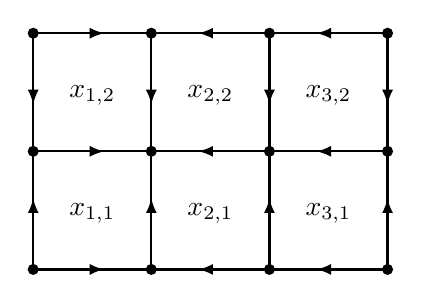
\begin{tikzpicture}[x=5mm, y=5mm, thick]
				\draw[myarrow=.6](0,0)--(0,3);
				\draw[myarrow=.6](3,0)--(3,3);
				\draw[myarrow=.6](6,0)--(6,3);
				\draw[myarrow=.6](9,0)--(9,3);
				\draw[myarrow=.6](0,6)--(0,3);
				\draw[myarrow=.6](3,6)--(3,3);
				\draw[myarrow=.6](6,6)--(6,3);
				\draw[myarrow=.6](9,6)--(9,3);
				%
				\draw[myarrow=.6](0,0)--(3,0);
				\draw[myarrow=.6](0,3)--(3,3);
				\draw[myarrow=.6](0,6)--(3,6);
				\draw[myarrow=.6](6,0)--(3,0);
				\draw[myarrow=.6](6,3)--(3,3);
				\draw[myarrow=.6](6,6)--(3,6);
				\draw[myarrow=.6](9,0)--(6,0);
				\draw[myarrow=.6](9,3)--(6,3);
				\draw[myarrow=.6](9,6)--(6,6);
				%
				\fill[black](0,0) circle(2pt);
				\fill[black](3,0) circle(2pt);
				\fill[black](6,0) circle(2pt);
				\fill[black](9,0) circle(2pt);
				\fill[black](0,3) circle(2pt);
				\fill[black](3,3) circle(2pt);
				\fill[black](6,3) circle(2pt);
				\fill[black](9,3) circle(2pt);
				\fill[black](0,6) circle(2pt);
				\fill[black](3,6) circle(2pt);
				\fill[black](6,6) circle(2pt);
				\fill[black](9,6) circle(2pt);
				%
				\draw(1.5,0.9) node[above]{$x_{1,1}$};
				\draw(4.5,0.9) node[above]{$x_{2,1}$};
				\draw(7.5,0.9) node[above]{$x_{3,1}$};
				\draw(1.5,3.9) node[above]{$x_{1,2}$};
				\draw(4.5,3.9) node[above]{$x_{2,2}$};
				\draw(7.5,3.9) node[above]{$x_{3,2}$};
			\end{tikzpicture}
		\end{figure}
	\end{example}
	
	
	
	We introduce some operators on grids, which are similar to the cubical operators. Let $X$ be a cubical set, and $(x,s)$ an $n$-grid of size $(l_1,\ldots,l_n)$ in $X$ for $n\ge 1$. If $s_{k}=0$ for all $k$, then $(x,s)$ is called \emph{directed}. A \emph{subgrid} of $(x,s)$ is a restriction of $(x,s)$, which itself forms a grid in $X$. We define $(x,s)\partial_{k,\alpha}$ as the $(n-1)$-grid $(y,t)$ of size $(l_1,\ldots,l_{k-1},l_{k+1},\ldots,l_n)$ such that
	\begin{align*}
		&y(i_1,\ldots,i_{k-1},i_{k+1},\ldots,i_n)\\
		&=
		\begin{cases}
			x(i_1,\ldots,i_{k-1},1,i_{k+1},\ldots,i_n)\partial_{k,s_k(1)}&(\alpha=0)\\
			x(i_1,\ldots,i_{k-1},l_k,i_{k+1},\ldots,i_n)\partial_{k,1-s_k(l_k)}&(\alpha=1)
		\end{cases}\\
		t&=(s_1,\ldots,s_{k-1},s_{k+1},\ldots,s_n).
	\end{align*}
	We also define $(x,s)\sigma_{k,\alpha}$ for $\alpha=0,1$ as the $(n+1)$-grid $(y,t)$ of size $(l_1,\ldots,l_{k-1},1,l_k,\ldots,l_n)$ such that
	\begin{align*}
		y(i_1,\ldots,i_{k-1},1,i_k,\ldots,i_n)&=x(i_1,\ldots,i_n)\sigma_k\\
		t&=(s_1,\ldots,s_{k-1},\alpha,s_{k},\ldots,s_n).
		%  \bar{t}&=(s_1,\ldots,s_{k-1},1,s_{k},\ldots,s_n).
	\end{align*}
	We finally define $(x,s)\gamma_{k,\alpha}$ as the $(n+1)$-grid $(y,t)$ of size $(l_1,\ldots,l_{k-1},l_k,l_k,l_{k+1},\ldots,l_n)$ such that
	\begin{align*}
		y(i_1,\ldots,i_{k-1},j_0,j_1,i_{k+1},\ldots,i_n)&=
		\begin{cases}
			x(i_1,\ldots,i_{k-1},j_{1-\alpha},i_{k+1},\ldots,i_n)\sigma_{k+\alpha}&(j_0<j_1)\\
			x(i_1,\ldots,i_{k-1},j_0,i_{k+1},\ldots,i_n)\gamma_{k,\alpha}&(j_0=j_1)\\
			x(i_1,\ldots,i_{k-1},j_\alpha,i_{k+1},\ldots,i_n)\sigma_{k+1-\alpha}&(j_0>j_1)
		\end{cases}\\
		t&=(s_1,\ldots,s_{k-1},s_k,s_k,s_{k+1},\ldots,s_n).
	\end{align*}
	It is straightforward to verify that faces and connections satisfy the cubical identities. However, the cubical identities involving degeneracies do not hold in general. %\tong{Remark that the degeneracies $\sigma_k$ in Section 6 will be consisting of $\sigma_{k,\alpha}$ such that the cubical identities involving the degeneracies hold. }
	The boundary of $(x,s)$ is defined as the subset of $(x,s)$ such that
	\[
	\partial(x,s)=\bigcup_{i,\alpha}(x,s)\partial_{i,\alpha}.
	\]
	Let $f\colon X\to Y$ be a cubical map. For every $n$-grid $(x,s)$ of size $(l_1,\ldots,l_n)$ in $X$, $f(x,s)=(f(x),s)$ is an $n$-grid of size $(l_1,\ldots,l_n)$ in $Y$. Moreover, if $\partial(x,s)$ is contained in a cubical subset $A\subset X$, then $f(x,s)$ is contained in $f(A)$.
	
	
	
	Next, we introduce the concatenation of grids. Geometrically, gluing two cubes of the same dimension along a common face yields a new cube. The concatenation of grids serves as a combinatorial abstraction of this observation, which was originally introduced in \cite{BHS} to define cubical \(\omega\)-groupoids.
	\begin{definition}
		Let $x=(x,s)$ and $y=(y,t)$ be $n$-grids of size $(l_1,\ldots,l_n)$ and $(m_1,\ldots,m_n)$ in a cubical set $X$ for $n\ge 1$. For $k=1,\ldots,n$, whenever $x\partial_{k,1}=y\partial_{k,0}$, we define $x+_ky$ as the $n$-grid $(z,u)$ such that
		\begin{align*}
			z(i_1,\ldots,i_n)&=
			\begin{cases}
				x(i_1,\ldots,i_n)&(i_k\le l_k)\\
				y(i_1,\ldots,i_{k-1},i_k-l_k,i_{k+1},\ldots,i_n)&(i_k>l_k)
			\end{cases}\\
			u(i_1,\ldots,i_n)&=
			\begin{cases}
				s(i_1,\ldots,i_n)&(i_k\le l_k)\\
				t(i_1,\ldots,i_{k-1},i_k-l_k,i_{k+1},\ldots,i_n)&(i_k>l_k).
			\end{cases}
		\end{align*}
	\end{definition}
	
	
	
	It is straightforward to verify that $+_k$ is associative and satisfies an interchange law
	\begin{equation}
		\label{interchange law}
		(x_1+_ky_1)+_l(x_2+_ky_2)=(x_1+_lx_2)+_k(y_1+_ly_2)
	\end{equation}
	for $k\ne l$. Let $x=(x,s)$ be an $n$-grid of size $(l_1,\ldots,l_n)$. For $k=1,\ldots,n$ and $j=1,\ldots,l_k$, we define the \emph{slice} $x[k,j]$ of $x$ as the $n$-grid $(y,t)$ of size $(l_1,\ldots,l_{k-1},1,l_{k+1},\ldots,l_n)$ such that
	\begin{align*}
		y(i_1,\ldots,i_{k-1},1,i_{k+1},\ldots,i_n)&=x(i_1,\ldots,i_{k-1},j,i_{k+1},\ldots,i_n)\\
		t&=(s_1,\ldots,s_{k-1},t_k,s_{k+1},\ldots,s_n)
	\end{align*}
	where 
	\[
	t_k\colon\{1\}\to\{s_k(j)\}.
	\]
	By definition, $x[k,j]+_kx[k,j+1]$ is well defined for $j=1,\ldots,l_k-1$. Next we introduce some equivalence relations between grids. We write
	\[
	x\xrightarrow{k}y
	\]
	for $n$-grids $x$ and $y$ if $x[k,j]=z\sigma_{k,\alpha}$ for some $(n-1)$-grid $z$, and
	\[
	y=x[k,1]+_k\cdots+_kx[k,j-1]+_kx[k,j+1]+_k\cdots+_kx[k,l_k],
	\]
	where $x$ is of size $(l_1,\ldots,l_n)$. If $x=x_1\xrightarrow{k_1}\cdots\xrightarrow{k_{m-1}}x_m=y$ for some $x_1,\ldots,x_m$ and $k_1,\ldots,k_{m-1}$, then we write $x\ge y$. Clearly, this provides a poset structure on the set of $n$-grids.
	
	
	
	\begin{definition}
		\label{0homotopy}
		We say that $n$-grids $x$ and $y$ are \emph{$0$-homotopic} if there exist $n$-grids $x_1,\ldots,x_k$ in $X$ such that $x=x_1$, $y=x_k$, and for each $i=1,\ldots,k-1$, either $x_i\le x_{i+1}$ or $x_i\ge x_{i+1}$ holds. In this case, we write $x\simeq_0y$.
	\end{definition}
	
	
	
	In other words, 0-homotopy only inserts or deletes degenerate slices of a grid. Let $x$ and $y$ be $n$-grids of the same size $(l_1,\ldots,l_n)$ in a cubical set $X$. If there exists an $(n+1)$-grid $z$ of size $(l_1,\ldots,l_{k-1},1,l_k,\ldots,l_n)$ such that $z\partial_{k,0}=x$ and $z\partial_{k,1}=y$, then we write
	\[
	x\overset{k}{\Rightarrow}y.
	\]
	
	
	
	\begin{definition}
		\label{1homotopy}
		We say that $n$-grids $x$ and $y$ are \emph{$1$-homotopic} if there exist $n$-grids $x_1,\ldots,x_k$ in $X$ such that $x=x_1$, $y=x_k$, and for each $i=1,\ldots,k-1$, either $x_i\overset{l_i}{\Rightarrow}x_{i+1}$ or $x_{i+1}\overset{l_i}{\Rightarrow}x_i$ holds for some $l_i$. In this case, we write $x\simeq_1y$.
	\end{definition}
	
	
	
	\begin{definition}
		\label{homotopy grids def}
		We say that $n$-grids $x$ and $y$ are \emph{homotopic} if there exist $n$-grids $x_1,\ldots,x_k$ such that $x=x_1$, $y=x_k$, and for each $i=1,\ldots,k-1$, either $x_i\simeq_0x_{i+1}$ or $x_i\simeq_1x_{i+1}$ holds. In this case, we write $x\simeq y$.
	\end{definition}
	Note that 0-homotopy, 1-homotopy and homotopy are equivalence relations between grids.
	
	
	\begin{remark}
		In \cite{KT}, the authors defined a $C_r$-homotopy for $r\ge 0$ between paths in a directed graph, and proved the Hurewicz theorem in dimension one and the Seifert-van Kampen theorem for the $r$-fundamental group defined by $C_r$-homotopies. A $0$-homotopy and a homotopy between $1$-grids correspond to a $C_0$-homotopy and a $C_2$-homotopy, respectively.
	\end{remark}
	
	
	
	The following lemma is immediate from the definition.
	
	
	
	\begin{lemma}
		\label{homotopy description}
		Let $X$ be a cubical set. Two $n$-grids $x$ and $y$ are homotopic if and only if there exist $n$-grids $z$ and $w$ such that
		\[
		x\le z\simeq_1 w\ge y.
		\]
	\end{lemma}
	
	
	
	Let $(X,x_0)$ be a pointed cubical set. We say that an $n$-grid $x$ in $X$ is \emph{spherical} if the boundary $\partial x$ consists of $x_0\sigma_{1}\cdots\sigma_{n-1}$. The set of spherical $n$-grids is closed under $0$-homotopy. We define a $1$-homotopy of spherical grids in the obvious manner. Hence we obtain a homotopy of spherical grids.
	
	
	
	\begin{definition}
		Let $(X,x_0)$ be a pointed cubical set. For $n\ge 0$, the $n$-th \emph{discrete homotopy group} $\pi_n^\delta(X,x_0)$ is defined as the set of homotopy classes of spherical grids.
	\end{definition}
	
	
	
	We define a group structure on $\pi_n^\delta(X,x_0)$ for $n\ge 1$. Let $x=(x,s)$ and $y=(y,t)$ be spherical $n$-grids of size $(l_1,\ldots,l_n)$ and $(m_1,\ldots,m_n)$ in a pointed cubical set $(X,x_0)$ for $n\ge 1$. Define the multiplication $x\cdot y$ as the spherical $n$-grid $(z,u)$ of size $(l_1+m_1,\ldots,l_n+m_n)$ such that
	\begin{align*}
		z(i_1,\ldots,i_n)&=
		\begin{cases}
			x(i_1,\ldots,i_n)&(i_1\le l_1,\ldots,i_n\le l_n)\\
			y(i_1-l_1,\ldots,i_n-l_n)&(i_1>l_1,\ldots,i_n>l_n)\\
			x_0\sigma_1\cdots\sigma_n&(\text{otherwise}),
		\end{cases}\\
		u_k(i_k)&=
		\begin{cases}
			s_k(i_k)&(i_k\le l_k)\\
			t_k(i_k-l_k)&(i_k>l_k).
		\end{cases}
	\end{align*}
	
	
	Thus the multiplication is obtained by placing the two spherical grids in diagonal blocks and sending all remaining blocks to the basepoint. The following lemma is immediate from the definitions of homotopies between grids and the multiplication of grids.
	
	
	
	\begin{lemma}
		\label{grid product}
		For $n\ge 1$ and $i=1,2$, let $x_i$ and $y_i$ be spherical $n$-grids in a pointed cubical set. If $x_1\simeq x_2$ and $y_1\simeq y_2$, then
		\[
		x_1\cdot y_1\simeq x_2\cdot y_2.
		\]
	\end{lemma}
	
	
	Next we show that the multiplication of grids is homotopic to the concatenation of grids along any direction. The idea is to slide the grids along any direction through homotopy.
	\begin{lemma}
		\label{grid slide}
		Let $x$ and $y$ be spherical $n$-grids in a pointed cubical set $(X,x_0)$. Then there exist spherical $n$-grids $a$ and $b$ of the same size such that $x\le a$, $y\le b$ and for each $i=1,\ldots,n$,
		\[
		x\cdot y\simeq a+_ib.
		\]
	\end{lemma}
	
	\begin{proof}
		Let $x=(x,s)$ and $y=(y,t)$. By inserting degenerate slices if necessary, we can construct $n$-grids $(a,u)$ and $(b,v)$ of the same size such that $u_1=\cdots=u_n=v_1=\cdots=v_n$, $x\le a$ and $y\le b$. We denote any $n$-grid consisting of $x_0\sigma_{1}\cdots\sigma_{n}$ simply by $x_0$. For $\{i_1<\cdots<i_k\}\subset\{1,\ldots,n\}$, we inductively define
		\[
		x+_{\{i_1,\ldots,i_k\}}y=(x+_{\{i_1,\ldots,i_{k-1}\}}x_0)+_{i_k}(x_0+_{\{i_1,\ldots,i_{k-1}\}}y).
		\]
		Then $x\cdot y=x+_{\{1,\ldots,n\}}y$. Note that
		\[
		((b\gamma_{j,1})+_j(b\gamma_{j,0}))\partial_{j+1,\alpha}=
		\begin{cases}
			x_0+_jb&(\alpha=0)\\
			b+_jx_0&(\alpha=1).
		\end{cases}
		\]
		Suppose $j>i$. Then we may define
		\[
		z=((a+_jx_0)\sigma_{j+1})+_{\{1,\ldots,j-1\}}((b\gamma_{j,1})+_j(b\gamma_{j,0})).
		\]
		By the interchange law \eqref{interchange law}, $z\partial_{j+1,\alpha}\simeq_0a+_{\{1,\ldots,j-\alpha\}}b$. Hence $a+_{\{1,\ldots,j-1\}}b\simeq a+_{\{1,\ldots,j\}}b$. Suppose $j<i$. We may also define
		\[
		w=((a+_{\{1,\ldots,j\}}x_0)\sigma_{j+1})+_{i+1}(x_0+_{\{1,\ldots,j-1\}}((b\gamma_{j,1})+_j(b\gamma_{j,0}))).
		\]
		By the interchange law, $w\partial_{j+1,\alpha}\simeq_0a+_{\{1,\ldots,j-\alpha,i\}}b$. Hence $a+_{\{1,\ldots,j-1,i\}}b\simeq a+_{\{1,\ldots,j,i\}}b$. Consequently,
		\[
		x\cdot y=x+_{\{1,\ldots,n\}}y\simeq a+_ib.
		\]
		Therefore the claim follows.
	\end{proof}
	
	
	
	We show that the multiplication above admits an inverse. Let $x=(x,s)$ be a spherical $n$-grid of size $(l_1,\ldots,l_n)$. Define an $n$-grid $\bar{x}=(\bar{x},\bar{s})$ by
	\[
	\bar{x}(i_1,\ldots,i_n)=x(i_1,\ldots,i_{n-1},l_n+1-i_n)\quad\text{and}\quad\bar{s}=(s_1,\ldots,s_{n-1},1-s_n),
	\]
	where $s=(s_1,\ldots,s_n)$.
	
	
	
	\begin{lemma}
		\label{grid inverse}
		For every spherical $n$-grid $x=(x,s)$, we have
		\[
		x\cdot\bar{x}\simeq x_0\simeq \bar{x}\cdot x.
		\]
	\end{lemma}
	
	\begin{proof}
		Consider an $(n+1)$-grid $y=(x{\gamma_{n,1}})+_{n+1}(\overline{x{\gamma_{n,1}}})$. By definition,
		\[
		y\partial_{i,\alpha}=\begin{cases}
			x+_n\bar{x}&((i,\alpha)=(n,1))\\
			x_0&\text{(otherwise)},
		\end{cases}
		\]
		which implies that $x\cdot\bar{x}\simeq x_0$ by Lemma \ref{grid slide}. Since $\overline{\bar{x}}=x$, we also obtain $\bar{x}\cdot x\simeq x_0$.
	\end{proof}
	
	
	
	\begin{proposition}
		Let $(X,x_0)$ be a pointed cubical set. Then for $n\ge 1$,
		\[
		\pi_n^\delta(X,x_0)\times\pi_n^\delta(X,x_0)\to\pi_n^\delta(X,x_0),\quad([x],[y])\mapsto[x\cdot y]
		\]
		is a well defined group structure.
	\end{proposition}
	
	\begin{proof}
		By Lemma \ref{grid product}, the multiplication is well defined. By definition, the multiplication is associative, and by Lemma \ref{grid inverse}, admits an inverse.
	\end{proof}
	
	
	
	Let $f\colon(X,x_0)\to(Y,y_0)$ be a pointed cubical map between pointed cubical sets $(X,x_0)$ and $(Y,y_0)$. Let $x$ and $y$ be spherical $n$-grids in $(X,x_0)$. Then $f(x)$ is a spherical $n$-grid in $(Y,y_0)$. Clearly, if spherical $n$-grids $x$ and $y$ in $(X,x_0)$ are homotopic, then $f(x)$ and $f(y)$ are also homotopic. Moreover, one has $f(x\cdot y)=f(x)\cdot f(y)$. Hence the map
	\[
	f_*\colon\pi_n^\delta(X,x_0)\to\pi_n^\delta(Y,y_0),\quad[x]\mapsto[f(x)]
	\]
	is a well defined homomorphism. By definition, the induced homomorphisms on discrete homotopy groups satisfy functoriality. %Pointed elementary homotopy, pointed homotopy, and pointed homotopy equivalence may be defined analogously to their unpointed counterparts.
	
	
	
	\begin{proposition}
		\label{homotopy invariance}
		Let $f,g\colon(X,x_0)\to(Y,y_0)$ be pointed cubical maps between pointed cubical sets. If there exists a pointed elementary homotopy from $f$ to $g$, then
		\[
		f_*=g_*\colon\pi_*^\delta(X,x_0)\to\pi_*^\delta(Y,y_0).
		\]
	\end{proposition}
	
	\begin{proof}
		Let $h\colon(X\otimes\Box^1,x_0\otimes\Box^1)\to(Y,y_0)$ be a pointed elementary homotopy from $f$ to $g$. For every spherical $n$-grid $(x,s)$ in $(X,x_0)$,
		\[
		f(x,s)\overset{n+1}{\Rightarrow}g(x,s)
		\]
		as spherical grids. Hence $[f(x,s)]=[g(x,s)]$ in $\pi_n^\delta(Y,y_0)$, and therefore the claim follows.
	\end{proof}
	
	\begin{corollary}
			\label{dhg under he}
			Let $(X,x_0)$, $(Y,y_0)$ be pointed cubical sets. If $(X,x_0)$ and $(Y,y_0)$ have the same pointed homotopy type, then there is an isomorphism
			\[
			\pi_n^\delta(X,x_0)\cong\pi_n^\delta(Y,y_0).
			\]
	\end{corollary}
	
	\begin{proposition}
		Let $(X,x_0)$ be a pointed cubical set. For $n\ge 2$, $\pi_n^\delta(X,x_0)$ is an abelian group.
	\end{proposition}
	
	\begin{proof}
		Let $x$ and $y$ be spherical $n$-grids in $(X,x_0)$, and let $a$ and $b$ be as in Lemma \ref{grid slide}. Since $n\ge 2$,
		\[
		x\cdot y\simeq a+_nb=\overline{\bar{b}+_n\bar{a}}\simeq \overline{\bar{b}+_1\bar{a}}\simeq b+_1a\simeq y\cdot x.
		\]
		Hence, for $n\ge 2$, $\pi_n^\delta(X,x_0)$ is an abelian group.
	\end{proof}
	%	As we showed above, the discrete homotopy groups can be defined for an arbitrary cubical set $X$, and they enjoy similar properties with the homotopy groups of a topological space. We will see their power in Theorems \ref{main 1} and \ref{main 3} when $X$ is quasisymmetric. However, the discrete homotopy groups are quite mysterious when $X$ is not quasisymmetric. We lack examples of cubical sets with nontrivial higher discrete homotopy groups, and more remain to be explore such as the comparison of $\pi_*^\delta(X,x_0)$ with those of its fibrant replacement, and the existence of homotopy operations, such as the action of $\pi_*^\delta(X,x_0)$ on $\pi_*^\delta(X,x_0)$. The authors believe this is a rich and interesting topic to work with.
	
	
	
	
	
	
	%	It is straightforward to define such actions in dimensions \(1\) and \(2\). However, for dimensions \(n\ge 3\), it is unclear how to proceed, because arbitrary cubical sets need not have coordinate-permutation symmetries.
	%	We may let \(\pi_1^\delta(X,x_0)\) act on itself by conjugation. For $*=2$, we may define the action as follows. Let $a\in\pi_1^\delta(X,x_0)$ and $$
	%	We currently lack examples of non-quasisymmetric cubical sets with nontrivial higher discrete homotopy groups, and much remains to be explored. Open questions include the comparing \(\pi_*^\delta(X,x_0)\) with the discrete homotopy groups of its fibrant replacement, as well as the existence of homotopy operations, such as the action of \(\pi_1^\delta(X,x_0)\) on \(\pi_*^\delta(X,x_0)\). 
	
	
	\section{Quasisymmetric cubical sets}\label{Quasisymmetric cubical sets}
	
	In this section, we introduce the notion of quasisymmetric cubical sets, which are cubical sets equipped with coordinate permutation symmetries that are required to be compatible with faces and degeneracies, but not necessarily with connections. We also introduce signed quasisymmetric cubical sets which are quasisymmetric cubical sets additionally equipped with symmetries by reversing cube coordinates. We then give a purely combinatorial construction of the left adjoint of the forgetful functor from the category of quasisymmetric cubical sets to $\cSet$, and show that the unit of this adjunction is an objectwise weak equivalence.
	
	
	\subsection{Symmetric and signed symmetric cubical sets}
	
	Let $\Sigma_n$ denote the $n$-th symmetric group for $n\ge 1$, and set $\Sigma_0=\{1\}$. %We assume that $\Sigma_n$ acts on $\{1,\ldots,n\}$ from the right. Hence for $\kappa,\lambda\in\Sigma_n$ and $i\in\{1,\ldots,n\}$, we have
	%\[
	%  (\lambda\kappa)(i)=\kappa(\lambda(i)).
	%\]
	We define the following maps:
	\begin{itemize}
		\item (permutations) $\kappa\colon[1]^n\to[1]^n$ for $\kappa\in\Sigma_n$ is given by
		\[
		\kappa(x_1,\ldots,x_n)=(x_{\kappa(1)},\ldots,x_{\kappa(n)}).
		\]
	\end{itemize}
	For $\kappa,\lambda\in\Sigma_n$, let
	\[
	(\kappa\lambda)(x_1,\ldots,x_n)=\kappa(\lambda(x_1,\ldots,x_n)).
	\]
	Then we have
	\[
	(\kappa\lambda)(i)=\lambda(\kappa(i))
	\]
	for $i=1,\ldots,n$. The \emph{symmetric cubical category} $\Box_\mathsf{sym}$ is defined by adjoining the maps $\kappa$, for all $\kappa\in\Sigma_n$ and all $n\ge 0$, to the cubical category $\Box$. The symmetric cubical category was introduced by Grandis and Mauri \cite{GM1}, who referred to it as the extended cubical category. Since we will consider a further extension of the cubical category, we adopt the terminology symmetric cubical category for $\Box_\mathsf{sym}$.
	
	
	
	For $i=1,\ldots,n$ and $\kappa\in\Sigma_n$, define $\kappa^{(i)}\in\Sigma_{n-1}$ by
	\[
	\kappa^{(i)}(j)=
	\begin{cases}
		\kappa(j)&(j<i,\,\kappa(j)<\kappa(i))\\
		\kappa(j)-1&(j<i,\,\kappa(j)>\kappa(i))\\
		\kappa(j+1)&(j\ge i,\,\kappa(j)<\kappa(i))\\
		\kappa(j+1)-1&(j\ge i,\,\kappa(j)>\kappa(i)).
	\end{cases}
	\]
	Namely, $\kappa^{(i)}$ is the restriction of $\kappa$ to the map $\{1,\ldots,n\}-\{i\}\to\{1,\ldots,n\}-\{\kappa(i)\}$ together with the identification $\{1<\ldots<n\}-\{k\}=\{1<\ldots<n-1\}$ as chains. Note that for $\kappa,\lambda\in\Sigma_n$ and $i=1,\ldots,n$,
	\begin{equation}
		\label{permutation deletion}
		(\kappa\lambda)^{(i)}=\kappa^{(i)}\lambda^{(\kappa(i))}.
	\end{equation}
	For $\kappa\in\Sigma_n$ and $p,q\in\{1,\ldots,n+1\}$, define $\kappa_{(p,q)}\in\Sigma_{n+1}$ by
	\[
	\kappa_{(p,q)}(p)=q\quad\text{and}\quad(\kappa_{(p,q)})^{(p)}=\kappa.
	\]
	It is straightforward to verify the identities
	\begin{equation}
		\label{permutation identity 1}
		\kappa\partial_{\kappa(i),\alpha}=\partial_{i,\alpha}\kappa^{(i)},\quad\kappa^{(i)}\sigma_{\kappa(i)}=\sigma_i\kappa
	\end{equation}
	and
	\begin{equation}
		\label{permutation identity 2}
		\kappa\gamma_{\kappa(i),\alpha}=\gamma_{i,\alpha}\kappa_{(i+1,\kappa(i)+1)},\quad\gamma_{i,\alpha}(i\,i+1)=\gamma_{i,\alpha}
	\end{equation}
	hold, where $(i\;i+1)$ denotes the transposition of $i$ and $i+1$. Alternatively, we may write \eqref{permutation identity 2} as the following identities
	\begin{equation}
		\label{permutation identity 2 alternative}
		\gamma_{i,\alpha}\kappa_{(i+1,\kappa(i)+1)}=\kappa\gamma_{\kappa(i),\alpha}=\gamma_{i,\alpha}\kappa_{(i+1,\kappa(i))}.
	\end{equation}
	Analogously to the cubical category $\Box$, the symmetric cubical category $\Box_\mathsf{sym}$ may be regarded as the category whose objects are $[1]^n$ for $n\ge 0$ and whose morphisms are freely generated by faces, degeneracies, connections and permutations, subject to the cubical identities together with the identities \eqref{permutation identity 1} and \eqref{permutation identity 2}.
	
	
	
	\begin{definition}
		The category $\SymcSet$ is the functor category $\mathsf{Set}^{\Box_\mathsf{sym}^\mathrm{op}}$. The objects and morphisms of $\SymcSet$ are referred to as \emph{symmetric cubical sets} and \emph{symmetric cubical maps}.
	\end{definition}
	
	
	
	\begin{example}
		The singular functor $\mathrm{Sing}\colon\mathsf{Top}\to\cSet$ factors through $\SymcSet$.
	\end{example}
	
	
	Isaacson \cite{I} showed that there is a model category structure on $\SymcSet$ such that the forgetful functor $\SymcSet\to\cSet$ is a Quillen equivalence, where $\cSet$ is equipped with the model category structure of Theorem \ref{cSet model structure}. Consequently, symmetric cubical sets also provide a model for the homotopy theory of spaces. An analogue of this result for cubical sets without connections was proved in \cite[Theorem 5.9]{Ar}.
	
	
	
	Recall that the $n$-th \emph{signed symmetric group} $B_n$ is the group of signed permutations on $\{\pm 1,\ldots,\pm n\}$. Namely, $B_n$ is the wreath product $\Z_2\wr\Sigma_n$. Hence, $B_n=(\Z_2)^n\times\Sigma_n$ as a set such that the product is given by
	\[
	(a,\kappa)(b,\lambda)=(a\kappa(b),\kappa\lambda)
	\]
	for $(a,\kappa),(b,\lambda)\in B_n$, where $\Sigma_n$ permutes coordinates of $(\Z_2)^n$. Set $\Z_2=\{0,1\}$, and for $a\in(\Z_2)^n$, write $a=(a_1,\ldots,a_n)$. We define the following map:
	\begin{itemize}
		\item (signed permutations) $(a,\kappa)\colon[1]^n\to[1]^n$ for $(a,\kappa)\in B_n$ is given by
		\[
		(a,\kappa)(x_1,\ldots,x_n)=(x_{\kappa(1)}^{a_1},\ldots,x_{\kappa(n)}^{a_n})
		\]
		where for $x\in[1]$, we set $x^0=x$ and $x^1=1-x$.
	\end{itemize}
	Define the \emph{signed symmetric cubical category} $\Box_\mathsf{sym}^\pm$ as the category obtained from $\Box_\mathsf{sym}$ by adjoining signed permutations.
	
	
	
	
	For $(a,\kappa)\in B_n$ and $i=\pm 1,\ldots,\pm n$, define $(a,\kappa)^{(i)}\in B_{n-1}$ by
	\[
	(a,\kappa)^{(i)}(j)=
	\begin{cases}
		(-1)^{a_j}\kappa(j)&(j<i,\,\kappa(j)<\kappa(i))\\
		(-1)^{a_j}(\kappa(j)-1)&(j<i,\,\kappa(j)\ge\kappa(i))\\
		(-1)^{a_{j+1}}\kappa(j+1)&(j\ge i,\,\kappa(j)<\kappa(i))\\
		(-1)^{a_{j+1}}(\kappa(j+1)-1)&(j\ge i,\,\kappa(j)\ge\kappa(i)).
	\end{cases}
	\]
	where $j=\pm 1,\ldots,\pm n$. Analogously to \eqref{permutation deletion}, for $(a,\kappa),(b,\lambda)\in B_n$ and $i=\pm 1,\ldots,\pm n$, we have
	\[
	((a,\kappa)(b,\lambda))^{(i)}=(a,\kappa)^{(i)}(b,\lambda)^{(\kappa(i))}.
	\]
	For $(a,\kappa)\in B_n$, $p,q\in\{1,\ldots,n+1\}$ and $\alpha=0,1$, define $(a,\kappa)_{(p,q),\alpha}\in B_{n+1}$ by
	\[
	((a,\kappa)_{(p,q),\alpha})(p)=(-1)^\alpha q\quad\text{and}\quad((a,\kappa)_{(p,q),\alpha})^{(p)}=(a,\kappa).
	\]
	It is straightforward to verify that the identities
	\begin{equation}
		\label{signed permutation identity 1}
		(a,\kappa)\partial_{\kappa(i),\alpha+a_i}=\partial_{i,\alpha}(a,\kappa)^{(i)},\quad(a,\kappa)^{(i)}\sigma_{\kappa(i)}=\sigma_i(a,\kappa)
	\end{equation}
	and
	\begin{equation}
		\label{signed permutation identity 2}
		(a,\kappa)\gamma_{\kappa(i),\alpha+a_i}=\gamma_{i,\alpha}(a,\kappa)_{(i+1,\kappa(i)+1),a_i},\quad\gamma_{i,\alpha}(0,(i\,i+1))=\gamma_{i,\alpha}.
	\end{equation}
	Analogously to the symmetric cubical category $\Box_\mathsf{sym}$, the signed symmetric cubical category $\Box_\mathsf{sym}^\pm$ may be regarded as the category whose objects are $[1]^n$ for $n\ge0$ and whose morphisms are freely generated by faces, degeneracies, connections and signed permutations, subject to the cubical identities together with the identities \eqref{signed permutation identity 1} and \eqref{signed permutation identity 2}.
	
	
	
	\begin{definition}
		The category $\SymcSet^\pm$ is the functor category $\mathsf{Set}^{(\Box_\mathsf{sym}^\pm)^\mathrm{op}}$. The objects and morphisms of $\SymcSet^\pm$ are referred to as \emph{signed symmetric cubical sets} and \emph{signed symmetric cubical maps}.
	\end{definition}
	
	
	
	\subsection{Quasisymmetric and signed quasisymmetric cubical sets}
	
	We define the quasisymmetric cubical category.
	
	
	
	\begin{definition}
		The \emph{quasisymmetric cubical category} $\Box_\mathsf{qsym}$ is defined as the category whose objects are $[1]^n$ for $n\ge 0$ and whose morphisms are freely generated by faces, degeneracies, connections and permutations subject to the cubical identities together with the identity \eqref{permutation identity 1}.
	\end{definition}
	
	
	
	Note that we are not imposing the identities \eqref{permutation identity 2} for the quasisymmetric cubical category. By definition, there is a sequence of the canonical functors
	\[
	\Box\to\Box_\mathsf{qsym}\to\Box_\mathsf{sym}.
	\]
	
	
	
	\begin{definition}
		The category $\QSymcSet$ is the functor category $\mathsf{Set}^{\Box_\mathsf{qsym}^\mathrm{op}}$. The objects and morphisms of $\QSymcSet$ are referred to as \emph{quasisymmetric cubical sets} and \emph{quasisymmetric cubical maps}.
	\end{definition}
	
	
	
	
	Quasisymmetric cubical sets have the following property that significantly simplifies homotopy theory of grids.
	
	
	
	\begin{proposition}
		\label{symmetric homotopy}
		Let $X$ be a quasisymmetric cubical set. For $n$-grids $x$ and $y$ in $X$, we have $x\overset{n+1}{\Rightarrow}y$ if and only if $x\overset{i}{\Rightarrow}y$ for some $i\in\{1,\ldots,n+1\}$.
	\end{proposition}
	
	\begin{proof}
		Suppose that $x\overset{i}{\Rightarrow}y$ for some $i$. Then there exists an $(n+1)$-grid $z$ such that $z\partial_{i,0}=x$ and $z\partial_{i,1}=y$. Let 
		\[\kappa=\begin{pmatrix}
			1&2&\cdots&i-1&i&i+1&\cdots&n+1\\
			1&2&\cdots&i-1&n+1&i&\cdots&n
		\end{pmatrix}
		\in\Sigma_{n+1}.
		\]
		Since $\kappa^{(i)}=1$, we have
		\[
		(z\kappa)\partial_{n+1,\alpha}=(z\kappa)\partial_{\kappa(i),\alpha}=(z\partial_{i,\alpha})\kappa^{(i)}=z\partial_{i,\alpha}.
		\]
		Hence $x\overset{n+1}{\Rightarrow}y$. Thus the if part is proved. The only if part is obvious.
	\end{proof}
	
	
	
	\begin{definition}
		The \emph{signed quasisymmetric cubical category} $\Box_\mathsf{qsym}^\pm$ is defined as the category whose objects are $[1]^n$ for $n\ge 0$ and whose morphisms are freely generated by faces, degeneracies, connections and signed permutations subject to the cubical identities together with the identity \eqref{signed permutation identity 1}.
	\end{definition}
	
	
	
	Note that we are not imposing the identities \eqref{signed permutation identity 2} for signed quasisymmetric cubical category. By definition, there is a canonical functor
	\[
	\Box_\mathsf{qsym}^\pm\to\Box_\mathsf{sym}^\pm.
	\]
	
	
	
	\begin{definition}
		The category $\QSymcSet^\pm$ is the functor category $\mathsf{Set}^{(\Box_\mathsf{qsym}^\pm)^\mathrm{op}}$. The objects and morphisms of $\QSymcSet^\pm$ are referred to as \emph{signed quasisymmetric cubical sets} and \emph{signed quasisymmetric cubical maps}.
	\end{definition}
	We will see in Remark \ref{quasisymm vs symm} that only the identities \eqref{signed permutation identity 1} are necessary for the Kan condition, which is why we work with (signed) quasisymmetric cubical sets rather than (signed) symmetric ones.
	
	
	\subsection{The functor $\mathcal{S}$}
	
	We define a functor $\mathcal{S}\colon\cSet\to\QSymcSet$ and prove Theorem \ref{main 2}. 
	
	
	
	\begin{definition}
		Define a functor $\mathcal{S}\colon\cSet\to\QSymcSet$ by setting $\mathcal{S}X_n=X_n\times\Sigma_n$ subject to the identification
		\begin{equation}
			\label{identification S}
			(x\sigma_p,\kappa_{(p,q)})=(x\sigma_1,\kappa_{(1,q)})
		\end{equation}
		for all $\kappa\in\Sigma_n$, $x\in X_n$ and $p,q=1,\ldots,n+1$, where faces, degeneracies and connections are defined by
		\begin{align*}
			(x,\kappa)\partial_{i,\alpha}&=(x\partial_{\kappa^{-1}(i),\alpha},\kappa^{(\kappa^{-1}(i))})\\
			(x,\kappa)\sigma_i&=(x\sigma_1,\kappa_{(1,i)})\\
			(x,\kappa)\gamma_{i,\alpha}&=(x\gamma_{\kappa^{-1}(i),\alpha},\kappa_{(\kappa^{-1}(i)+1,i+1)}).
		\end{align*}
	\end{definition}
	\begin{remark}
		Although we do not require \eqref{permutation identity 2} (or, equivalently, \eqref{permutation identity 2 alternative}) to hold here, the reader may notice that the definition of the connections in \(\mathcal{S}X\) is precisely the first identity in \eqref{permutation identity 2 alternative}. In fact, \(\mathcal{S}X\) carries an alternative cubical set structure in which the connections are defined by the second identity in \eqref{permutation identity 2 alternative} instead of the first. Either of these two cubical set structures is suitable for our purposes, as they are isomorphic to each other, and the identities in \eqref{permutation identity 2 alternative} play no role in the remainder of this paper.
	\end{remark}
	
	
	
	
	
	We denote an element of $\mathcal{S}X_n$ represented by $(x,\kappa)\in X_n\times\Sigma_n$ by the same symbol $(x,\kappa)$.
	
	
	
	\begin{lemma}
		The functor $\mathcal{S}\colon\cSet\to\QSymcSet$ is well defined.
	\end{lemma}
	
	\begin{proof}
		Let $X$ be a cubical set. It suffices to show that $\mathcal{S}X$ is a well defined quasisymmetric cubical set. Let $(x,\kappa)\in\mathcal{S}X_n$ and $i,p,q\in\{1,\ldots,n+1\}$. We have
		\[
		\kappa_{(p,q)}^{-1}(i)=
		\begin{cases}
			\kappa^{-1}(i)&(i<q\text{ and }\kappa^{-1}(i)<p)\\
			\kappa^{-1}(i)+1&(i<q\text{ and }\kappa^{-1}(i)\ge p)\\
			p&(i=q)\\
			\kappa^{-1}(i-1)&(i>q\text{ and }\kappa^{-1}(i-1)<p)\\
			\kappa^{-1}(i-1)+1&(i>q\text{ and }\kappa^{-1}(i-1)\ge p).
		\end{cases}
		\]
		Suppose that $i<q$ and $\kappa^{-1}(i)<p$. Then
		\begin{align*}
			(x\sigma_p,\kappa_{(p,q)})\partial_{i,\alpha}&=(x\sigma_p\partial_{\kappa^{-1}(i),\alpha},(\kappa_{(p,q)})^{(\kappa^{-1}(i))})\\
			&=(x\partial_{\kappa^{-1}(i),\alpha}\sigma_{p-1},(\kappa^{(\kappa^{-1}(i))})_{(p-1,q-1)})\\
			&=(x\partial_{\kappa^{-1}(i),\alpha}\sigma_{1},(\kappa^{(\kappa^{-1}(i))})_{(1,q-1)})\\
			&=(x\sigma_{1}\partial_{\kappa^{-1}(i)+1,\alpha},(\kappa_{(1,q)})^{(\kappa^{-1}(i)+1)})\\
			&=(x\sigma_1,\kappa_{(1,q)})\partial_{i,\alpha}.
		\end{align*}
		Similarly,
		\begin{align*}
			(x\sigma_p,\kappa_{(p,q)})\sigma_i&=(x\sigma_p\sigma_1,(\kappa_{(p,q)})_{(1,i)})\\
			&=(x\sigma_1\sigma_{p+1},(\kappa_{(1,i)})_{(p+1,q+1)})\\
			&=(x\sigma_1\sigma_{2},(\kappa_{(1,i)})_{(2,q+1)})\\
			&=(x\sigma_1\sigma_1,(\kappa_{(1,q)})_{(1,i)})\\
			&=(x\sigma_1,\kappa_{(1,q)})\sigma_i
		\end{align*}
		and
		\begin{align*}
			(x\sigma_p,\kappa_{(p,q)})\gamma_{i,\alpha}&=(x\sigma_p\gamma_{\kappa^{-1}(i),\alpha},(\kappa_{(p,q)})_{(\kappa^{-1}(i)+1,i+1)})\\
			&=(x\gamma_{\kappa^{-1}(i),\alpha}\sigma_{p+1},(\kappa_{(\kappa^{-1}(i),i)})_{(p+1,q+1)})\\
			&=(x\gamma_{\kappa^{-1}(i),\alpha}\sigma_1,(\kappa_{(\kappa^{-1}(i),i)})_{(1,q+1)})\\
			&=(x\sigma_1\gamma_{\kappa^{-1}(i)+1,\alpha},(\kappa_{(1,q)})_{(\kappa^{-1}(i)+1,i)})\\
			&=(x\sigma_1,\kappa_{(1,q)})\gamma_{i,\alpha}.
		\end{align*}
		Thus $(x,\kappa)\partial_{i,\alpha}$, $(x,\kappa)\sigma_i$ and $(x,\kappa)\gamma_{i,\alpha}$ are well defined in this case. The remaining cases are verified in the same manner. We now verify the cubical identity. For $j\le i$,
		\begin{align*}
			(x,\kappa)\sigma_i\sigma_j&=(x\sigma_1\sigma_1,(\kappa_{(1,i)})_{(1,j)})\\
			&=(x\sigma_1\sigma_2,(\kappa_{(1,j)})_{(2,i+1)})\\
			&=(x\sigma_1\sigma_1,(\kappa_{(1,j)})_{(1,i+1)})\\
			&=(x,\kappa)\sigma_{j}\sigma_{i+1}.
		\end{align*}
		The remaining identities are verified analogously. Hence $\mathcal{S}X$ is a well-defined cubical set.
		
		
		
		Next, define an action of $\Sigma_n$ on $\mathcal{S}X_n$ by
		\[
		(x,\kappa)\lambda=(x,\kappa\lambda)
		\]
		for $\lambda\in\Sigma_n$ and $(x,\kappa)\in\mathcal{S}X_n$. Since
		\[
		(x\sigma_1,\kappa_{(1,q)})\lambda=(x\sigma_1,(\kappa\lambda^{(q)})_{(1,\lambda(q))})=(x\sigma_p,(\kappa\lambda^{(q)})_{(p,\lambda(q))})=(x\sigma_p,\kappa_{(p,q)})\lambda
		\]
		for $(x,\kappa)\in\mathcal{S}X_n$ and $\lambda\in\Sigma_{n+1}$, this action is well defined. By \eqref{permutation deletion}, we have
		\[
		((x,\kappa)\partial_{i,\alpha})\lambda^{(i)}=(x\partial_{\kappa^{-1}(i),\alpha},\kappa^{(\kappa^{-1}(i))}\lambda^{(i)})=(x\partial_{\kappa^{-1}(i),\alpha},(\kappa\lambda)^{(\kappa^{-1}(i))})=((x,\kappa)\lambda)\partial_{\lambda(i),\alpha}
		\]
		for $(x,\kappa)\in\mathcal{S}X_n$ and $\lambda\in\Sigma_n$. We also have
		\[
		((x,\kappa)\sigma_i)\mu=(x\sigma_i,\kappa_{(i,i)})\mu=(x\sigma_i,(\kappa\mu^{(i)})_{(i,\mu(i))})=(x\sigma_{\mu(i)},(\kappa\mu^{(i)})_{(\mu(i),\mu(i))})=((x,\kappa)\mu^{(i)})\sigma_{\mu(i)}
		\]
		for $(x,\kappa)\in\mathcal{S}X_n$ and $\mu\in\Sigma_{n+1}$. Therefore $\mathcal{S}X$ is a well defined quasisymmetric cubical set.
	\end{proof}
	
	
	
	By definition, the functor $\mathcal{S}$ is the left adjoint of the forgetful functor $\mathcal{U}\colon\QSymcSet\to\cSet$. Moreover, the cubical maps
	\[
	X\to\mathcal{U}\mathcal{S}X,\quad x\mapsto(x,1)
	\]
	form the unit of this adjunction. We show that the unit $\eta\colon 1_\cSet\Rightarrow\mathcal{US}$ is an objectwise weak equivalence. Our method is to show that $|X|$ is a deformation retract of $|\mathcal{US}X|$ by constructing homotopies locally. For $\kappa\in\Sigma_n$, define $\bar{\kappa}\in\Sigma_{2n}$ by setting
	\[
	\bar{\kappa}(i)=
	\begin{cases}
		i&(i=2j-1)\\
		2\kappa(j)&(i=2j).
	\end{cases}
	\]
	We now construct a deformation that moves each permuted cube to its canonical representative while remaining compatible with the cubical structure. Let $X$ be a cubical set. For $(x,\kappa)\in X_n\times\Sigma_n$, let $Q(x,\kappa)=(x\gamma_{n,1}\cdots\gamma_{1,1},\bar{\kappa})$ and define a map $h(x,\kappa)\colon|(x,\kappa)|\times[0,1]\to|Q(x,\kappa)|$ by
	\begin{align*}
		&h(x,\kappa)(x_1,\ldots,x_n,t)\\
		&=
		\begin{cases}
			(x_{\kappa(1)},2(x_1-1)t+1,\ldots,x_{\kappa(n)},2(x_n-1)t+1)&(0\le t\le\frac{1}{2})\\
			(2(1-x_{\kappa(1)})t+2x_{\kappa(1)}-1,x_1,\ldots,2(1-x_{\kappa(n)})t+2x_{\kappa(n)}-1,x_n)&(\frac{1}{2}\le t\le 1).
		\end{cases}
	\end{align*}
	Set $\bar{h}(x,\kappa)=\rho\circ h(x,\kappa)\colon|(x,\kappa)|\times[0,1]\to|\mathcal{US}X|$.
	
	
	
	\begin{lemma}
		\label{S t=0,1}
		Let $X$ be a cubical set. For every $(x,\kappa)\in X_n\times\Sigma_n$, $\bar{h}(x,\kappa)(-,t)$ coincides with the composite
		\[
		|(x,\kappa)|\xrightarrow{\kappa}|(x,1)|\xrightarrow{\rho}|\mathcal{US}X|\quad\text{and}\quad|(x,\kappa)|\xrightarrow{\rho}|\mathcal{US}X|
		\]
		for $t=0,1$, respectively, where $\kappa\colon|(x,\kappa)|\to|(x,1)|$ denotes the self-map of $[0,1]^n$ that permutes coordinates by $\kappa$.
	\end{lemma}
	
	\begin{proof}
		By the cubical identity,
		\[
		Q(x,\kappa)\partial_{2,1}\cdots\partial_{n+1,1}=(x,1)\quad\text{and}\quad Q(x,\kappa)\partial_{1,1}\cdots\partial_{n,1}=(x,\kappa).
		\]
		Hence the claim follows.
	\end{proof}
	
	
	
	\begin{lemma}
		\label{S gluing}
		Let $X$ be a cubical set, and let $(x,\kappa)\in X_n\times\Sigma_n$. For all $i$ and $\alpha$, the diagrams
		\[
		\xymatrix{
			|(x,\kappa)\partial_{i,\alpha}|\times[0,1]\ar[d]_{\partial_{i,\alpha}\times 1}\ar[rr]^(.6){\bar{h}((x,\kappa)\partial_{i,\alpha})}&&|\mathcal{US}X|\ar@{=}[d]\\
			|(x,\kappa)|\times[0,1]\ar[rr]^(.57){\bar{h}(x,\kappa)}&&|\mathcal{US}X|
		}
		\qquad
		\xymatrix{
			|(x,\kappa)\sigma_i|\times[0,1]\ar[d]_{\sigma_i\times 1}\ar[rr]^(.59){\bar{h}((x,\kappa)\sigma_i)}&&|\mathcal{US}X|\ar@{=}[d]\\
			|(x,\kappa)|\times[0,1]\ar[rr]^(.57){\bar{h}(x,\kappa)}&&|\mathcal{US}X|
		}
		\]
		commute.
	\end{lemma}
	
	\begin{proof}
		For $\kappa\in\Sigma_n$, one has $(\bar{\kappa}^{(2j)})^{(2j-1)}=(\bar{\kappa}^{(2j-1)})^{(2j-1)}=\overline{\kappa^{(j)}}$. Suppose that $\alpha=1$ and $\kappa^{-1}(i)\le i$. By the cubical identity,
		\begin{align*}
			Q(x,\kappa)\partial_{2i,1}\partial_{2\kappa^{-1}(i)-1,1}&=(x\gamma_{n,1}\cdots\gamma_{1,1}\partial_{2\kappa^{-1}(i),1}\partial_{2\kappa^{-1}(i)-1,1},(\bar{\kappa}^{(2\kappa^{-1}(i))})^{(2\kappa^{-1}(i)-1)})\\
			&=(x\partial_{\kappa^{-1}(i),1}\gamma_{n-1,1}\cdots\gamma_{1,1},\overline{\kappa^{(\kappa^{-1}(i))}})\\
			&=Q((x,\kappa)\partial_{i,1}).
		\end{align*}
		Hence the left diagram commutes. The case that $\alpha=1$ and $\kappa^{-1}(i)>i$ is proved analogously. Suppose that $\alpha=0$ and $0\le t\le\frac{1}{2}$. By the cubical identity,
		\begin{align*}
			Q(x,\kappa)\partial_{2\kappa^{-1}(i)-1,0}&=(x\gamma_{n,1}\cdots\gamma_{1,1}\partial_{2\kappa^{-1}(i)-1,0},\bar{\kappa}^{(2\kappa^{-1}(i)-1)})\\
			&=(x\partial_{\kappa^{-1}(i),0}\gamma_{n,1}\cdots\gamma_{1,1}\sigma_{2\kappa^{-1}(i)-1},\bar{\kappa}^{(2\kappa^{-1}(i)-1)})\\
			&=Q((x,\kappa)\partial_{i,0})\sigma_{2i-1}.
		\end{align*}
		Hence the left diagram commutes. The case that $\alpha=0$ and $\frac{1}{2}\le t\le 1$ is proved analogously.
		
		
		
		By the cubical identities,
		\[
		Q((x,\kappa)\sigma_i)=(x\sigma_i\gamma_{n+1,1}\cdots\gamma_{1,1},\overline{\kappa_{(i,i)}})=(x\gamma_{n,1}\cdots\gamma_{1,1}\sigma_{2i-1}\sigma_{2i},\overline{\kappa_{(i,i)}})=Q(x,\kappa)\sigma_{2i-1}\sigma_{2i}.
		\]
		Hence the right diagram commutes.
	\end{proof}
	We are ready to prove Theorem \ref{main 2}.
	
	
	%	\begin{proposition}
		%		\label{S}
		%		The unit $\eta\colon 1_\cSet\Rightarrow\mathcal{US}$ is an objectwise weak equivalence.
		%	\end{proposition}
	
	\begin{proof}
		[Proof of Theorem \ref{main 2}]
		Let $X$ be a cubical set. By Lemmas \ref{S t=0,1} and \ref{S gluing}, the family of homotopies $\{\bar{h}(x,\kappa)\}$, where $(x,\kappa)$ ranges over all elements of $X_n\times\Sigma_n$ for $n\ge 0$, assembles to a homotopy $\bar{h}\colon|\mathcal{US}X|\times[0,1]\to|\mathcal{US}X|$ satisfying that $\bar{h}(-,1)=1_{|\mathcal{US}X|}$ and $\bar{h}(-,0)$ factors as
		\[
		|\mathcal{US}X|\xrightarrow{f}|X|\xrightarrow{\eta}|\mathcal{US}X|
		\]
		such that $f\circ\eta=1_{|X|}$. Therefore $f$ is a homotopy inverse of $\eta\colon|X|\to|\mathcal{US}X|$.
	\end{proof}
	
	
	
	\section{Fibrant replacement}\label{Fibrant replacement}
	
	In this section, we explicitly construct a fibrant replacement for a quasisymmetric cubical set, which is the key ingredient in proving Theorems \ref{main 1} and \ref{main 3}.
	
	
	
	\subsection{The functor $\mathcal{R}$}
	
	To construct a fibrant replacement, we first need a mechanism to formally invert cubes. We define a functor $\mathcal{R}\colon\cSet\to\cSet$ by reversing cube coordinates. Reversing cube coordinates plays an important role in several contexts, including cubical $\omega$-groupoids in \cite{BHS}.
	
	
	
	\begin{definition}
		We define a functor
		\[
		\mathcal{R}\colon\cSet\to\cSet
		\]
		by setting $\mathcal{R}X_0=X_0$ and
		\[
		\mathcal{R}X_n=\{x^{s_1\cdots s_n}\mid x\in X_n\text{ and }s_1,\ldots,s_n\in\{0,1\}\}
		\]
		for $n\ge 1$, subject to the identification
		\begin{equation}
			\label{R identification}
			(x\sigma_i)^{s_1\cdots s_{i-1}0s_{i+1}\cdots s_n}=(x\sigma_i)^{s_1\cdots s_{i-1}1s_{i+1}\cdots s_n}.
		\end{equation}
		Faces, degeneracies, and connections are defined by
		\begin{align*}
			(x^{s_1\cdots s_n})\partial_{i,\alpha}&=(x\partial_{i,s_i(1-\alpha)+(1-s_i)\alpha})^{s_1\cdots s_{i-1}s_{i+1}\cdots s_n}\\
			(x^{s_1\cdots s_n})\sigma_i&=(x\sigma_i)^{s_1\cdots s_{i-1}0s_{i}\cdots s_n}\\
			(x^{s_1\cdots s_n})\gamma_{i,\alpha}&=(x\gamma_{i,s_i(1-\alpha)+(1-s_i)\alpha})^{s_1\cdots s_is_i\cdots s_n}.
		\end{align*}
	\end{definition}
	
	
	
	Let $X$ be a cubical set. For any $n$-cube $x\in X_n$, the element $x^{s_1\cdots s_n}\in\mathcal{R}X_n$ may be interpreted as the $n$-cube obtained by reversing the $i$-th coordinate of $x$ for each $i$ with $s_i=1$. More precisely, the assignment
	\[
	x^{s_1\cdots s_n}\mapsto(x,(s_1,\ldots,s_n))
	\]
	yields a one-to-one correspondence between $\mathcal{R}X_n$ and the set of $n$-grids in $X$ of size $(1,\ldots,1)$ subject to the identification $x\sigma_{i,0}=x\sigma_{i,1}$.
	
	
	
	\begin{lemma}
		The functor $\mathcal{R}$ is well defined.
	\end{lemma}
	
	\begin{proof}
		Let $X$ be a cubical set. It suffices to show that $\mathcal{R}X$ is a well-defined cubical set. Let $x\in X_{n-1}$, $i\in\{1,...,n\}$ and $s_1,\ldots,s_{i-1},s_{i+1},\ldots,s_n\in\{0,1\}$. Suppose that $j<i$. Then
		
		\begin{align*}
			(x\sigma_i)^{s_1\cdots s_{i-1}0s_{i+1}\cdots s_n}\partial_{j,\alpha}&=(x\sigma_i\partial_{j,s_j(1-\alpha)+(1-s_j)\alpha})^{s_1\cdots s_{j-1}s_{j+1}\cdots s_{i-1}0s_{i+1}\cdots s_n}\\
			&=(x\partial_{j,s_j(1-\alpha)+(1-s_j)\alpha}\sigma_{i-1})^{s_1\cdots s_{j-1}s_{j+1}\cdots s_{i-1}0s_{i+1}\cdots s_n}\\
			&=(x\partial_{j,s_j(1-\alpha)+(1-s_j)\alpha}\sigma_{i-1})^{s_1\cdots s_{j-1}s_{j+1}\cdots s_{i-1}1s_{i+1}\cdots s_n}\\
			&=(x\sigma_{i}\partial_{j,s_j(1-\alpha)+(1-s_j)\alpha})^{s_1\cdots s_{j-1}s_{j+1}\cdots s_{i-1}1s_{i+1}\cdots s_n}\\
			&=(x\sigma_i)^{s_1\cdots s_{i-1}1s_{i+1}\cdots s_n}\partial_{j,\alpha}.
		\end{align*}
		The remaining cases are verified in the same manner. Hence faces are well defined. It is analogously proved that degeneracies and connections are well defined. We now verify the cubical identity. Let $x^{s_1\cdots s_n}\in\mathcal{R}X_n$. For $j\le i$,
		\begin{align*}
			(x^{s_1\cdots s_n})\partial_{j,\beta}\partial_{i,\alpha}&=((x\partial_{j,s_j(1-\beta)+(1-s_j)\beta})^{s_1\cdots s_{j-1}s_{j+1}\cdots s_n})\partial_{i,\alpha}\\
			&=(x\partial_{j,s_j(1-\beta)+(1-s_j)\beta}\partial_{i,s_{i+1}(1-\alpha)+(1-s_{i+1})\alpha})^{s_1\cdots s_{j-1}s_{j+1}\cdots s_{i}s_{i+2}\cdots s_n}\\
			&=(x\partial_{i+1,s_{i+1}(1-\alpha)+(1-s_{i+1})\alpha}\partial_{j,s_j(1-\beta)+(1-s_j)\beta})^{s_1\cdots s_{j-1}s_{j+1}\cdots s_{i-1}s_{i+1}\cdots s_n}\\
			&=((x\partial_{i+1,s_{i+1}(1-\alpha)+(1-s_{i+1})\alpha})^{s_1\cdots s_{i-1}s_{i+1}\cdots s_n})\partial_{j,\beta}\\
			&=(x^{s_1\cdots s_n})\partial_{i+1,\alpha}\partial_{j,\beta}.
		\end{align*}
		One also has
		\begin{align*}
			(x^{s_1\cdots s_n})\gamma_{i,\alpha}\partial_{i,1-\alpha}&=((x\gamma_{i,s_i(1-\alpha)+(1-s_i)\alpha})^{s_1\cdots s_is_is_{i+1}\cdots s_n})\partial_{i,\alpha}\\
			&=(x\gamma_{i,s_i(1-\alpha)+(1-s_i)\alpha}\partial_{i,s_i\alpha+(1-s_i)(1-\alpha)})^{s_1\cdots s_n}\\
			&=(x\partial_{i,s_i\alpha+(1-s_i)(1-\alpha)}\sigma_i)^{s_1\cdots s_n}\\
			&=((x\partial_{i,s_i\alpha+(1-s_i)(1-\alpha)})^{s_1\cdots s_is_i\cdots s_n})\sigma_i\\
			&=x^{s_1\cdots s_n}\partial_{i,1-\alpha}\sigma_i,
		\end{align*}
		where we use the identification \eqref{R identification} for the fourth equality. The remaining cubical identities are verified analogously, and therefore the claim follows.
	\end{proof}
	
	
	
	Define the natural transformation $\iota\colon 1_{\cSet}\Rightarrow\mathcal{R}$ by
	\[
	\iota\colon X\to\mathcal{R}X,\quad x\mapsto x^{0\cdots 0}.
	\]
	It is straightforward to verify that $\iota$ is well defined. We show that $\iota$ is an objectwise weak equivalence by arguing similarly to the proof of Theorem \ref{main 2}. Let $X$ be a cubical set. For $x^{s_1\cdots s_n}\in\mathcal{R}X_n$ with $n\ge 1$, let $Q(x^{s_1\cdots s_n})=(x\gamma_{n,1}\cdots\gamma_{1,1})^{0s_10s_2\cdots0s_n}$. We define a map
	\[
	h(x^{s_1\cdots s_n})\colon|x^{s_1\cdots s_n}|\times[0,1]\to|Q(x^{s_1\cdots s_n})|
	\]
	by
	\begin{align*}
		&h(x^{s_1\cdots s_n})(x_1,\ldots,x_n,t)\\
		&=
		\begin{cases}
			(\bar{x}_1,2(x_1+s_1-1)t+1-s_1,\ldots,\bar{x}_n,2(x_n+s_n-1)t+1-s_n)&(0\le t\le\frac{1}{2})\\
			(2(1-\bar{x}_1)t+2\bar{x}_1-1,x_1,\ldots,2(1-\bar{x}_n)t+2\bar{x}_n-1,x_n)&(\frac{1}{2}\le t\le 1)
		\end{cases}
	\end{align*}
	where $\bar{x}_i=(1-s_i)x_i+s_i(1-x_i)$. For $y\in \mathcal{R}X_0=X_0$, we define $h(y)\colon|y|\times[0,1]\to|y|$ as the projection. For every $z\in\mathcal{R}X$, set
	\[
	\bar{h}(z)=\rho\circ h(z)\colon|z|\times[0,1]\to|\mathcal{R}X|.
	\]
	
	
	
	\begin{lemma}
		\label{R t=0,1}
		Let $X$ be a cubical set. For every $x^{s_1\cdots s_n}\in\mathcal{R}X_n$, $\bar{h}(x^{s_1\cdots s_n})(-,t)$ coincides with
		\[
		|x^{s_1\cdots s_n}|\xrightarrow{m_{s_1\cdots s_n}}|x^{0\cdots 0}|\xrightarrow{\rho}|\mathcal{R}X|\quad\text{and}\quad|x^{s_1\cdots s_n}|\xrightarrow{\rho}|\mathcal{R}X|
		\]
		for $t=0,1$, respectively, where
		\[
		m_{s_1\cdots s_n}(x_1,\ldots,x_n)=(\bar{x}_1,\ldots,\bar{x}_n).
		\]
	\end{lemma}
	
	\begin{proof}
		For $n=0$, the claim is obvious. Assume $n\ge 1$, and let $x^{s_1\cdots s_n}\in\mathcal{R}X_n$. By definition,
		\[
		h(x^{s_1\cdots s_n})(x_1,\ldots,x_n,0)=(\bar{x}_1,1-s_1,\ldots,\bar{x}_n,1-s_n)\in|Q(x^{s_1\cdots s_n})|.
		\]
		By the cubical identity,
		$(x\gamma_{n,1}\cdots\gamma_{1,1})^{0s_10s_2\cdots0s_n}\partial_{2,1-s_1}\cdots\partial_{n+1,1-s_n}=x^{0\cdots 0}$. Hence the claim for $t=0$ follows. The claim for $t=1$ is proved analogously.
	\end{proof}
	
	
	
	\begin{lemma}
		\label{R gluing}
		Let $X$ be a cubical set, and let $z\in\mathcal{R}X_n$. For all $i$ and $\alpha$, the diagrams
		\[
		\xymatrix{
			|z\partial_{i,\alpha}|\times[0,1]\ar[d]_{\partial_{i,\alpha}\times 1}\ar[rr]^(.6){\bar{h}(z\partial_{i,\alpha})}&&|\mathcal{R}X|\ar@{=}[d]\\
			|z|\times[0,1]\ar[rr]^(.57){\bar{h}(z)}&&|\mathcal{R}X|
		}
		\qquad
		\xymatrix{
			|z\sigma_i|\times[0,1]\ar[d]_{\sigma_i\times 1}\ar[rr]^(.59){\bar{h}(z\sigma_i)}&&|\mathcal{R}X|\ar@{=}[d]\\
			|z|\times[0,1]\ar[rr]^(.57){\bar{h}(z)}&&|\mathcal{R}X|
		}
		\]
		commute.
	\end{lemma}
	
	\begin{proof}
		Let $x^{s_1\cdots s_n}\in\mathcal{R}X_n$. By the cubical identity,
		\[
		Q(x^{s_1\cdots s_n}\sigma_i)=Q(x^{s_1\cdots s_n})\sigma_{2i-1}\sigma_{2i}\quad\text{and}\quad Q(x^{s_1\cdots s_n})\partial_{2i,1-s_i}\partial_{2i-1,1}=Q(x^{s_1\cdots s_n}\partial_{i,1}).
		\]
		Hence the right diagram and the left diagram for $\alpha=1-s_i$ commute. By the cubical identity,
		\[
		Q(x^{s_1\cdots s_n})\partial_{2i-1,0}=Q((x^{s_1\cdots s_n})\partial_{i,0})\sigma_{2i-1}.
		\]
		Hence for $\alpha=s_i$ and $0\le t\le\frac{1}{2}$
		\begin{align*}
			&\bar{h}(x^{s_1\cdots s_n})\partial_{i,0}(x_1,\ldots,x_{i-1},x_{i+1},\ldots,x_n,t)\\
			&=\bar{h}(x^{s_1\cdots s_n})(x_1,\ldots,x_{i-1},0,x_{i+1},\ldots,x_n,t)\\
			&=\rho(\bar{x}_1,\tilde{x}_1,\ldots,\bar{x}_{i-1},\tilde{x}_{i-1},0,2(2s_i-1)t+1-s_i,\bar{x}_{i+1},\tilde{x}_{i+1},\ldots,\bar{x}_n,\tilde{x}_n)\\
			&=\rho(\bar{x}_1,\tilde{x}_1,\ldots,\bar{x}_{i-1},\tilde{x}_{i-1},\bar{x}_{i+1},\tilde{x}_{i+1},\ldots,\bar{x}_n,\tilde{x}_n)\\
			&=\bar{h}((x^{s_1\cdots s_n})\partial_{i,0})(x_1,\ldots,x_{i-1},x_{i+1},\ldots,x_n,t),
		\end{align*}
		where $\tilde{x}_k=2(x_k+s_k-1)t+1-s_k$ for $k=1,\ldots,i-1,i+1,\ldots,n$. Therefore the left diagram commutes for $\alpha=s_i$ and $0\le t\le\frac{1}{2}$. The case that $\alpha=s_i$ and $\frac{1}{2}\le t\le 1$ is proved analogously.
	\end{proof}
	
	
	
	\begin{proposition}
		\label{R}
		The natural transformation $\iota\colon 1_{\cSet}\Rightarrow\mathcal{R}$ is an objectwise weak equivalence.
	\end{proposition}
	
	\begin{proof}
		Let $X$ be a cubical set. By Lemmas \ref{R t=0,1} and \ref{R gluing}, the family of homotopies $\{\bar{h}(z)\}_{z\in\mathcal{R}X}$ assembles to a homotopy $\bar{h}\colon|\mathcal{R}X|\times[0,1]\to|\mathcal{R}X|$ satisfying that $\bar{h}(-,1)=1_{|\mathcal{R}X|}$ and $\bar{h}(-,0)$ factors as
		\[
		|\mathcal{R}X|\xrightarrow{f}|X|\xrightarrow{\iota}|\mathcal{R}X|
		\]
		such that $f\circ\iota=1_{|X|}$. Therefore $f$ is the homotopy inverse of $\iota\colon|X|\to|\mathcal{R}X|$.
	\end{proof}
	
	
	
	\subsection{The functor $\mathcal{G}$}
	
	We define a functor $\mathcal{G}\colon\cSet\to\cSet$ by constructing the cubical set of directed grids.
	
	
	
	\begin{definition}
		Define a functor
		\[
		\mathcal{G}\colon\cSet\to\cSet
		\]
		by setting $\mathcal{G}X_n$ to be the set of all directed $n$-grids in $X$ subject to the identification
		\begin{equation}
			\label{G identification}
			x\sigma_{i,0}+_ix\sigma_{i,0}=x\sigma_{i,0}
		\end{equation}
		for all directed $n$-grids $x$ and $i=1,\ldots,n$, where faces and connections are as in Section \ref{Discrete homotopy groups of cubical sets} and degeneracies are defined by
		\begin{align*}
			x\sigma_i&=x\sigma_{i,0}.
		\end{align*}
		
	\end{definition}
	
	
	
	\begin{lemma}
		\label{G well defined}
		The functor $\mathcal{G}$ is well defined.
	\end{lemma}
	
	\begin{proof}
		Let $X$ be a cubical set. It suffices to show that faces, degeneracies and connections are well defined on $\mathcal{G}X$. For every directed $n$-grid $x$ in $X$, one has
		\begin{align*}
			x\sigma_j\partial_{i,\alpha}&=
			\begin{cases}
				x\partial_{i,\alpha}\sigma_{j-1}&(i<j)\\
				x&(i=j)\\
				x\partial_{i-1,\alpha}\sigma_j&(i>j).
			\end{cases}
		\end{align*}
		and
		\begin{align*}
			(x\sigma_j+_jx\sigma_j)\partial_{i,\alpha}&=
			\begin{cases}
				x\partial_{i,\alpha}\sigma_{j-1}+_{j-1}x\partial_{i,\alpha}\sigma_{j-1}&(i<j)\\
				x&(i=j)\\
				x\partial_{i-1,\alpha}\sigma_j+_jx\partial_{i-1,\alpha}\sigma_j&(i>j).
			\end{cases}
		\end{align*}
		Hence faces are well defined. It is analogously proved that degeneracies and connections are well defined. One also has
		\begin{align*}
			(x\gamma_{k,\alpha}\partial_{k,1-\alpha})(i_1,\ldots,i_n)&=(x\gamma_{k,\alpha})(i_1,\ldots,i_{k-1},\alpha+(1-\alpha)l_k,i_k,\ldots,i_n)\partial_{k,1-\alpha}\\
			&=x(i_1,\ldots,i_{k-1},\alpha+(1-\alpha)l_k,i_{k+1},\ldots,i_n)\sigma_{k+1}\partial_{k,1-\alpha}\\
			&=(x\partial_{k,1-\alpha})(i_1,\ldots,i_{k-1},i_{k+1},\ldots,i_n)\sigma_k,
		\end{align*}
		which implies that
		\[
		(x\gamma_{k,\alpha}\partial_{k,1-\alpha})[k,j]=x\partial_{k,1-\alpha}\sigma_k
		\]
		for $j=1,\ldots,l_k$. Using the identification \eqref{G identification}, the cubical identity is easily verified. The remaining cubical identities are verified analogously, and therefore the claim follows.
	\end{proof}
	
	
	
	Define a natural transformation $\phi\colon 1_{\cSet}\Rightarrow\mathcal{G}$ by
	\[
	\phi\colon X\to\mathcal{G}X,\quad x\mapsto (x,0).
	\]
	It is immediate to verify that $\phi\colon X\to\mathcal{G}X$ is a cubical map for every cubical set $X$. Hence $\phi$ is well defined. We show that \(\phi\) is an objectwise weak equivalence by arguing similarly to the proof of Theorem \ref{main 2}.
	
	
	
	Let $X$ be a cubical set. For a directed $n$-grid $x$ of size $(l_1,\ldots,l_n)$ in $X$, we set $\|x\|=[0,l_1]\times\cdots\times[0,l_n]$. Faces and degeneracies on $\|x\|$ are defined in the obvious manner. We then define
	\[
	\|\mathcal{G}X\|=\left(\coprod_{x\in\mathcal{G}X}\|x\|\right)/\sim
	\]
	where the equivalence relation is generated by $\partial_{i,\alpha}\|x\|\sim\|x\partial_{i,\alpha}\|$ and $\sigma_i\|x\|\sim\|x\sigma_i\|$. One has that $\|\mathcal{G}X\|$ is well defined. For every directed grid $x$ in $X$, let $\rho\colon\|x\|\to\|\mathcal{G}X\|$ denote the canonical map. The canonical linear homeomorphisms $\|x\|\to|x|$ induce a natural homeomorphism
	\begin{equation}
		\label{G homeo}
		\|\mathcal{G}X\|\xrightarrow{\cong}|\mathcal{G}X|.
	\end{equation}
	
	
	
	Let $x$ be a directed $n$-grid of size $(l_1,\ldots,l_n)$ in $X$. Then one has a directed $n$-grid
	\[
	(\cdots((x\gamma_{1,1}\cdots\gamma_{n,1})[2,i_1])\cdots)[2n,i_n]
	\]
	of size $(l_1,1,\ldots,l_n,1)$. These are glued together to form
	\[
	Q(x)=\bigcup_{i_1=1}^{l_1}\cdots\bigcup_{i_n=1}^{l_n}\|(\cdots((x\gamma_{1,1}\cdots\gamma_{n,1})[2,i_1])\cdots)[2n,i_n]\|
	\]
	such that the maps  $\rho\colon\|(\cdots((x\gamma_{1,1}\cdots\gamma_{n,1})[2,i_1])\cdots)[2n,i_n]\|\to\|\mathcal{G}X\|$ for all $i_1,\ldots,i_n$ assemble to a map $\rho\colon Q(x)\to\|\mathcal{G}X\|$. Define a map $h(x)\colon\|x\|\times[0,1]\to Q(x)$ by
	\[
	h(x)(x_1,\ldots,x_n,t)=
	\begin{cases}
		(x_1,2(x_1-l_1)t+l_1,\ldots,x_n,2(x_n-l_n)t+l_n)&(0\le t\le\frac{1}{2})\\
		(2(l_1-x_1)t+2x_1-l_1,x_1,\ldots,2(l_n-x_n)t+2x_n-l_n,x_n)&(\frac{1}{2}\le t\le 1).
	\end{cases}
	\]
	We then set $\bar{h}(x)=\rho\circ h(x)$. The following lemma is immediate from the definition.
	
	
	
	\begin{lemma}
		\label{G t=0,1}
		Let $X$ be a cubical set, and let $x$ be a directed $n$-grid $x$ in $X$. Then
		\[
		\bar{h}(x)(-,0)=\rho\colon\|x\|\to\|\mathcal{G}X\|
		\]
		and $\bar{h}(x)(-,1)$ takes values in $\phi(|X|)\subset\|\mathcal{G}X\|$. Moreover, if $x$ is of size $(1,\ldots,1)$, then $\bar{h}(x)(-,1)$ coincides with the composite
		\[
		\|x\|=|x|\xrightarrow{\rho}|X|\xrightarrow{\phi}\|\mathcal{G}X\|.
		\]
	\end{lemma}
	
	
	
	
	The following lemma is proved quite analogously to Lemma \ref{R gluing}.
	
	
	
	\begin{lemma}
		\label{G gluing}
		Let $X$ be a cubical set, and let $x\in\mathcal{G}X_n$. For all $i$ and $\alpha$, the diagrams
		\[
		\xymatrix{
			\|x\partial_{i,\alpha}\|\times[0,1]\ar[d]_{\partial_{i,\alpha}\times 1}\ar[rr]^(.6){\bar{h}(x\partial_{i,\alpha})}&&\|\mathcal{G}X\|\ar@{=}[d]\\
			\|x\|\times[0,1]\ar[rr]^(.57){\bar{h}(x)}&&\|\mathcal{G}X\|
		}
		\qquad
		\xymatrix{
			\|x\sigma_i\|\times[0,1]\ar[d]_{\sigma_i\times 1}\ar[rr]^(.59){\bar{h}(x\sigma_i)}&&\|\mathcal{G}X\|\ar@{=}[d]\\
			\|x\|\times[0,1]\ar[rr]^(.57){\bar{h}(x)}&&\|\mathcal{G}X\|
		}
		\]
		commute.
	\end{lemma}
	
	\begin{proof}
		Let $x\in\mathcal{G}X_n$. By the cubical identity,
		\[
		Q(x\sigma_i)=Q(x)\sigma_{2i-1}\sigma_{2i}\quad\text{and}\quad Q(x)\partial_{2i,1}\partial_{2i-1,1}=Q(x\partial_{i,1}).
		\]
		Hence the right diagram commutes. One also has
		\[
		Q(x)\partial_{2i-1,0}=Q(x\partial_{i,0})\sigma_{2i-1}.
		\]
		Hence for $\alpha=0$ and $0\le t\le\frac{1}{2}$,
		\begin{align*}
			&\bar{h}(x)(x_1,\ldots,x_{i-1},0,x_{i+1},\ldots,x_n)\\
			&=\rho(x_1,\bar{x}_1,\ldots,x_{i-1},\bar{x}_{i-1},0,l_i-2l_it,x_{i+1},\bar{x}_{i+1},\ldots,x_n,\bar{x}_n)\\
			&=\rho(x_1,\bar{x}_1,\ldots,x_{i-1},\bar{x}_{i-1},\bar{x}_{i+1},\ldots,x_n,\bar{x}_n)
		\end{align*}
		where $\bar{x}_i=2(x_i-l_i)t+l_i$. Therefore the left diagram commutes for $\alpha=0$ and $0\le t\le\frac{1}{2}$. The remaining cases are proved analogously.
	\end{proof}
	
	
	
	\begin{proposition}
		\label{G}
		The natural transformation $\phi\colon 1_{\cSet}\Rightarrow\mathcal{G}$ is an objectwise weak equivalence.
	\end{proposition}
	
	\begin{proof}
		Let $X$ be a cubical set. By Lemmas \ref{G t=0,1} and \ref{G gluing}, the family of homotopies $\{\bar{h}(x)\}$, where $x$ ranges over all directed grids in $X$, assembles to a homotopy $\bar{h}\colon\|\mathcal{G}X\|\times[0,1]\to\|\mathcal{G}X\|$ satisfying that $\bar{h}(-,0)=1_{\|\mathcal{G}X\|}$ and $\bar{h}(-,1)$ factors as
		\[
		\|\mathcal{G}X\|\xrightarrow{f}|X|\xrightarrow{\phi}\|\mathcal{G}X\|
		\]
		such that $f\circ\phi=1_{|X|}$. Therefore $f$ is the homotopy inverse of $\phi\colon|X|\to\|\mathcal{G}X\|$. Composing with the homeomorphism \eqref{G homeo}, the claim follows.
	\end{proof}
	
	
	
	\subsection{The functor $\mathcal{G}_0$}
	
	We define a functor constructing the cubical set of 0-homotopy classes of directed grids.
	
	\begin{definition}
		Define a functor
		\[
		\mathcal{G}_0\colon\cSet\to\cSet
		\]
		by setting $\mathcal{G}_0X_n$ to be the set of all 0-homotopy classes of directed grids in $X$. Faces, degeneracies and connections are defined by
		\[
		[x]\partial_{i,\alpha}=[x\partial_{i,\alpha}],\quad[x]\sigma_i=[x\sigma_i],\quad[x]\gamma_{i,\alpha}=[x\gamma_{i,\alpha}].
		\]
	\end{definition}
	
	
	
	Since $x\sigma_i+_ix\sigma_i$ and $x\sigma_i$ are 0-homotopic, by Lemma \ref{G well defined}, the functor $\mathcal{G}_0$ is well defined and there is the canonical natural transformation $\pi\colon\mathcal{G}\Rightarrow\mathcal{G}_0$. We show that the natural transformation $\pi$ is an objectwise weak equivalence by applying Quillen's Theorem A. We start with the proof of Proposition \ref{realization connection} by Theorem A.
	
	
	
	Let $X$ be a cubical set. The \emph{cube category} $\Box\downarrow X$ is the category whose objects are cubical maps $\Box^n\to X$ for $n\ge 0$ and morphisms are commutative diagrams
	\begin{equation}
		\label{cube cat morphism}
		\xymatrix{
			\Box^m\ar[r]^\theta\ar[d]&\Box^n\ar[d]\\
			X\ar@{=}[r]&X
		}
	\end{equation}
	where $\theta$ is any cubical map. %By \cite[4.1. LEMMA]{GM}, the cube category $\Box\downarrow X$ admits standard factorizations.
	%\begin{lemma}
	%  \label{factorization without connections}
	%  Every morphism $f\colon(\Box^m\to X)\to(\Box^n\to X)$ in the cube category $\Box\downarrow X$ admits a unique factorization
	%  \[
	%    f=(\partial_{i_1,\alpha_1}\cdots\partial_{t_r,\alpha_r})(\sigma_{j_1}\cdots\sigma_{j_s}),
	%  \]
	%  where $i_1>\cdots>i_r$ and $k_1<\cdots<k_s$.
	%\end{lemma}
	Let $|\Box|\colon\Box\downarrow X\to\mathsf{Top}$ be a functor that assigns to every $\Box^n\to X$ the geometric $n$-cube $[0,1]^n$. Then the standard barycentric subdivision argument shows that there is a natural homeomorphism
	\begin{equation}
		\label{cube cat homeo}
		|X|_\gamma\cong\underset{\Box\downarrow X}{\mathrm{colim}}\,|\Box|.
	\end{equation}
	
	
	To prove Proposition \ref{realization connection}, we need the following proof, which is also proved in \cite[Proposition 3.12, Corollary 3.14]{ACK}.
	\begin{lemma}
		\label{cube cat hocolim}
		Let $X$ be a cubical set. Then the canonical map
		\[
		\underset{\Box\downarrow X}{\mathrm{hocolim}}\,|\Box|\to\underset{\Box\downarrow X}{\mathrm{colim}}\,|\Box|
		\]
		is a homotopy equivalence.
	\end{lemma}
	
	\begin{proof}
		We refer to \cite{H} for Reedy categories. By Lemma \ref{factorization}, the cube category $\mathcal{C}=\Box\downarrow X$ is a Reedy category such that $\overset{\rightarrow}{\mathcal{C}}$ consists of faces and $\overset{\leftarrow}{\mathcal{C}}$ consists of degeneracies and connections. Let $x\colon\Box^n\to X$ be an object of $\mathcal{C}$. Since the latching object for $x$ is $\partial|x|$, the functor $|\Box|$ is Reedy cofibrant. If $x$ is nondegenerate and not a connection, then the matching category of $\mathcal{C}$ at $x$ is empty. Suppose $x$ is degenerate or a connection. By Lemma \ref{factorization}, there is $y\in\Box\downarrow X$ such that $y$ is nondegenerate and not a connection, and $x$ is uniquely given by $$y(\gamma_{i_1,\alpha_1}\cdots\gamma_{i_r,\alpha_r})(\sigma_{j_1}\cdots\sigma_{j_s}),$$
		where $i_1\le\cdots\le i_r$ and $j_1<\cdots<j_s$ such that $\alpha_k\ne\alpha_{k+1}$ for $i_k=i_{k+1}$. Then the morphism
		\[
		(\gamma_{i_1,\alpha_1}\cdots\gamma_{i_r,\alpha_r})(\sigma_{j_1}\cdots\sigma_{j_s})\colon x\to y
		\]
		is the terminal object in the matching category of $\mathcal{C}$ at $x$. %Hence by the cubical identity, for any objects $y$ and $z$ of the matching category of $\mathcal{C}$ at $x$, there exists an object $w$ and morphisms
		%		\[
		%		y\to w\leftarrow z
		%		\]
		%		in the matching category of $\mathcal{C}$ at $x$. 
		Thus the matching category of $\mathcal{C}$ at $x$ is connected. Consequently, by \cite[Proposition 15.10.2]{H}, the Reedy category $\mathcal{C}$ has fibrant constants. Therefore by \cite[Proposition 19.9.1]{H}, the claim follows.
	\end{proof}
	
	
	
	For a small category $\mathcal{C}$, let $B\mathcal{C}$ denote the classifying space of $\mathcal{C}$, i.e. the simplicial geometric realization of the nerve of $\mathcal{C}$.
	
	
	
	\begin{lemma}
		\label{cube cat classifying space}
		Let $X$ be a cubical set. Then there is a natural homotopy equivalence
		\[
		|X|_\gamma\simeq B(\Box\downarrow X).
		\]
	\end{lemma}
	
	\begin{proof}
		By definition, $B(\Box\downarrow X)$ is the homotopy colimit of the constant functor over $\Box\downarrow X$. Hence by the homotopy invariance of homotopy colimits, there is a natural homotopy equivalence
		\[
		B(\Box\downarrow X)\simeq\underset{\Box\downarrow X}{\mathrm{hocolim}}\,|\Box|.
		\]
		The claim follows from Lemma \ref{cube cat hocolim}.
	\end{proof}
	
	
	
	We are ready to prove Proposition \ref{realization connection}.
	
	
	
	\begin{proof}
		[Proof of Proposition \ref{realization connection}]
		Let $X$ be a cubical set, and let $\overline{\Box\downarrow X}$ denote the category whose objects are cubical maps $\Box^n\to X$ and morphisms are commutative diagrams \eqref{cube cat morphism} such that $\theta$ is the composite of faces and degeneracies. Then
		\[
		\underset{\overline{\Box\downarrow X}}{\mathrm{colim}}\,|\Box|=|X|
		\]
		and analogously to Lemma \ref{cube cat classifying space}, we can show that
		\begin{equation}
			\label{realization classfying space without connections}
			|X|\simeq B(\overline{\Box\downarrow X}).
		\end{equation}
		Hence it is sufficient to show that the inclusion $\iota\colon\overline{\Box\downarrow X}\to\Box\downarrow X$ induces a homotopy equivalence on classifying spaces. For every cubical map $x\colon\Box^n\to X$, the comma category $\iota/x$ is isomorphic to $\overline{\Box\downarrow\Box^n}$ . The inclusion $\overline{\Box\downarrow\Box^n}\to\Box\downarrow\Box^n$ induces the quotient map
		\[
		|\Box^n|=\underset{\overline{\Box\downarrow \Box^n}}{\mathrm{colim}}\,|\Box|\to\underset{\Box\downarrow\Box^n}{\mathrm{colim}}\,|\Box|=|\Box^n|_\gamma.
		\]
		By \cite[Propositions 2.1 and 2.2]{A}, the quotient map induces isomorphisms in $\pi_1$ and homology. Clearly, $|\Box^n|_\gamma\cong[0,1]^n$ is contractible. Hence $|\Box^n|$ is also contractible, and by \eqref{realization classfying space without connections}, $B(\iota/x)\cong B(\overline{\Box\downarrow\Box^n})$ is also contractible. By Quillen's Theorem A, the map $\iota\colon B(\overline{\Box\downarrow X})\to B(\Box\downarrow X)$ is a homotopy equivalence.
	\end{proof}
	
	
	
	We characterize the 0-homotopy between directed grids as follows. For $n\ge 0$, let $[n]$ denote the poset $\{0<\cdots<n\}$. We call a surjective poset map $[m]\to[n]$ an \emph{expander}. Let $X$ be a cubical set, and let $\epsilon_i\colon[m_i]\to[l_i]$ be an expander. For a directed $n$-grid $x$ of size $(l_1,\ldots,l_n)$ in $X$, we define a directed $n$-grid $x^{\epsilon_i}$ of size $(l_1,\ldots,l_{i-1},m_i,l_{i+1},\ldots,l_n)$ by
	\[
	x^{\epsilon_i}=x_1+_i\cdots+_ix_n,
	\]
	where
	\[
	x_j=x[i,j]+_i\underbrace{(x[i,j]\partial_{i,1}\sigma_i)+_i\cdots+(x[i,j]\partial_{i,1}\sigma_i)}_{|\epsilon_i^{-1}(j)|-1}.
	\]
	We call $\epsilon=(\epsilon_1,\ldots,\epsilon_n)$ an \emph{$n$-expander}, and define
	\[
	x^\epsilon=(\cdots(x^{\epsilon_1})\cdots)^{\epsilon_n}.
	\]
	Clearly, one has $x\le x^\epsilon$. The following lemma is immediate from the definition.
	
	
	
	\begin{lemma}
		\label{expander}
		Let $X$ be a cubical set. If $n$-grids $x$ and $y$ in $X$ satisfy $x\le y$, then there exists an expander $\epsilon$ such that
		\[
		y=x^\epsilon.
		\]
	\end{lemma}
	
	
	
	Let $x$ be a directed $n$-grid of size $(l_1,\ldots,l_n)$. For $i=1,\ldots,n$, we say that $x$ is \emph{$i$-minimal} if $x[i,j]$ is nondegenerate for all $j=1,\ldots,l_i$. There exists a unique sequence $1\le j_1<\cdots<j_k\le l_i$ such that for $j\ne j_1,\ldots,j_k$, the slice $x[i,j]$ is degenerate. Hence
	\[
	x[i]=x[i,j_1]+_i\cdots+_ix[i,j_k]
	\]
	is $i$-minimal and 0-homotopic to $x$. Set
	\[
	x_{\mathrm{min}}=(\cdots(x[1])\cdots)[n]
	\]
	which is minimal, i.e. $i$-minimal for all $i=1,\ldots,n$. By Lemma \ref{expander}, we may define the expander $\epsilon(x)$ by
	\[
	x=(x_{\mathrm{min}})^{\epsilon(x)}.
	\]
	By definition, $\epsilon$ is unique. Clearly, directed $n$-grids $a$ and $b$ are 0-homotopic if and only if $a_{\mathrm{min}}=b_{\mathrm{min}}$. Hence for $y\in\mathcal{G}_0X$, we may define $y_\mathrm{min}\in\mathcal{G}X$ in the obvious manner.
	
	
	
	Let $X$ be a cubical set. Consider the functor $\pi\colon\Box\downarrow\mathcal{G}X\to\Box\downarrow\mathcal{G}_0X$. For $x\in\mathcal{G}_0X$, objects of the comma category $\pi/x$ are pairs $(\theta,y)$ of a morphism $\theta\colon\Box^m\to\Box^n$ and an object $y\in\mathcal{G}X_m$ such that $\pi(y)=x\theta$. In particular, $\pi/x$ is the cube category of the cubical set $\pi_x$ defined by the pullback of cubical sets
	\[
	\xymatrix{
		\pi_x\ar[r]\ar[d]&\Box^n\ar[d]^x\\
		\mathcal{G}X\ar[r]^\pi&\mathcal{G}_0X.
	}
	\]
	Every $m$-cube of $\pi_x$ is a pair $(\theta,y)$ as before, and faces, degeneracies and connections are defined by
	\begin{align*}
		(\theta,y)\partial_{i,\alpha}&=(\theta\partial_{i,\alpha},y\partial_{i,\alpha}),\\
		(\theta,y)\sigma_i&=(\theta\sigma_i,y\sigma_i),\\
		(\theta,y)\gamma_{i,\alpha}&=(\theta\gamma_{i,\alpha},y\gamma_{i,\alpha}).
	\end{align*}
	We aim to show that $|\pi_x|$ is contractible for all $x\in\mathcal{G}_0X$.
	
	
	
	Thus minimal representatives commute well with degeneracies and connections, but taking a face may create new degenerate slices; the following formulas record the required correction. Note that for $z\in\mathcal{G}X_n$ we have
	\[
	z_{\min}\partial_{i,\alpha}=((z\partial_{i,\alpha})_{\min})^{\epsilon(z_{\min}\partial_{i,\alpha})},
	\]
	and $\epsilon(z_{\min}\partial_{i,\alpha})$ is nontrivial in general. We also have
	\[
	z_{\min}{\sigma_i}=(z\sigma_i)_{\min},\quad z_{\min}\gamma_{i,\alpha}=(z\gamma_{i,\alpha})_{\min}.
	\]
	For an expander $\epsilon=(\epsilon_1,\ldots,\epsilon_n)$, define
	\begin{align*}
		\epsilon\partial_i&=(\epsilon_1,\ldots,\epsilon_{i-1},\epsilon_{i+1},\ldots,\epsilon_n)\\
		\epsilon\sigma_i&=(\epsilon_1,\ldots,\epsilon_{i-1},1,\epsilon_i,\ldots,\epsilon_n)\\
		\epsilon\gamma_i&=(\epsilon_1,\ldots,\epsilon_i,\epsilon_i,\ldots,\epsilon_n).
	\end{align*}
	Then by the uniqueness of $\epsilon(-)$ we have
	\begin{align*}
		\epsilon(z\partial_{i,\alpha})&=\epsilon(z_{\min}\partial_{i,\alpha})\circ(\epsilon(z)\partial_i),\\
		\epsilon(z\sigma_i)&=\epsilon(z)\sigma_i,\\
		\epsilon(z\gamma_{i,\alpha})&=\epsilon(z)\gamma_i.
	\end{align*}
	Then for
	\[
	\theta=(\partial_{i_1,\alpha_1}\cdots\partial_{i_r,\alpha_r})(\gamma_{j_1,\beta_1}\cdots\gamma_{j_s,\beta_s})(\sigma_{k_1}\cdots\sigma_{k_t})
	\]
	we have
	\[
	\epsilon(x_{\min}\theta)=\epsilon((x\partial_{i_1,\alpha_1}\cdots\partial_{i_r,\alpha_r})_{\min})(\gamma_{j_1}\cdots\gamma_{j_s})(\sigma_{k_1}\cdots\sigma_{k_t}).
	\]
	For expanders $\epsilon=(\epsilon_1,\ldots,\epsilon_n)$ and $\delta=(\delta_1,\ldots,\delta_n)$, we define an expander
	\[
	\epsilon\odot\delta=(\epsilon_1,\delta_1,\ldots,\epsilon_n,\delta_n).
	\]
	For $(\theta,y)\in(\pi_x)_m$, let
	\[
	Q(\theta,y)=(\theta\gamma_{m,1}\cdots\gamma_{1,1},(y_\mathrm{min}\gamma_{m,1}\cdots\gamma_{1,1})^{\epsilon(y)\odot\epsilon(x_\mathrm{min}\theta)})
	\]
	and define a map $h(\theta,y)\colon|(\theta,y)|\times[0,1]\to|Q(\theta,y)|$ by
	\begin{align*}
		&h(\theta,y)(x_1,\ldots,x_m,t)\\
		&=
		\begin{cases}
			(x_1,2(x_1-1)t+1,\ldots,x_m,2(x_m-1)t+1)&(0\le t\le\frac{1}{2})\\
			(2(1-x_1)t+2x_1-1,x_1,\ldots,2(1-x_m)t+2x_m-1,x_m)&(\frac{1}{2}\le t\le 1).
		\end{cases}
	\end{align*}
	Set $\bar{h}(\theta,y)=\rho\circ h(\theta,y)\colon|(\theta,y)|\times[0,1]\to|\pi_x|$. The following lemma is immediate from the definition.
	
	
	
	\begin{lemma}
		\label{G_0 t=0,1}
		Let $X$ be a cubical set. For every $x\in\mathcal{G}_0X$ and $(\theta,y)\in\pi_x$,
		\[
		\bar{h}(\theta,y)(-,0)=\rho\colon|(\theta,y)|\to|\pi_x|
		\]
		and $\bar{h}(\theta,y)(-,1)$ takes values in $|(1,x_\mathrm{min})|\subset|\pi_x|$. Moreover,
		\[
		\bar{h}(\theta,x_\mathrm{min}\theta)(-,1)=\rho\colon|(\theta,x_\mathrm{min}\theta)|\to|\pi_x|.
		\]
	\end{lemma}
	
	
	
	
	The following lemma is proved quite analogously to Lemma \ref{R gluing}.
	
	
	
	\begin{lemma}
		\label{G_0 gluing}
		Let $X$ be a cubical set. For every $x\in\mathcal{G}_0X$ and $(\theta,y)\in\pi_x$, the diagrams
		\[
		\xymatrix{
			|(\theta,y)\partial_{i,\alpha}|\times[0,1]\ar[d]_{\partial_{i,\alpha}\times 1}\ar[rr]^(.6){\bar{h}((\theta,y)\partial_{i,\alpha})}&&|\pi_x|\ar@{=}[d]\\
			|(\theta,y)|\times[0,1]\ar[rr]^(.57){\bar{h}(\theta,y)}&&|\pi_x|
		}
		\qquad
		\xymatrix{
			|(\theta,y)\sigma_i|\times[0,1]\ar[d]_{\sigma_i\times 1}\ar[rr]^(.59){\bar{h}((\theta,y)\sigma_i)}&&|\pi_x|\ar@{=}[d]\\
			|(\theta,y)|\times[0,1]\ar[rr]^(.57){\bar{h}(\theta,y)}&&|\pi_x|
		}
		\]
		commute.
	\end{lemma}
	
	\begin{proof}
		By Lemma \ref{factorization}, one has the standard factorization
		\[
		\theta=(\partial_{i_1,\alpha_1}\cdots\partial_{i_r,\alpha_r})(\gamma_{j_1,\beta_1}\cdots\gamma_{j_s,\beta_s})(\sigma_{k_1}\cdots\sigma_{k_t})
		\]
		where $m=n-t+s+r$. Again by Lemma \ref{factorization}, one also has the standard factorization
		\[
		(\gamma_{j_1,\beta_1}\cdots\gamma_{j_s,\beta_s})(\sigma_{k_1}\cdots\sigma_{k_t})\partial_{i,\alpha}=\partial_{i',\alpha'}(\gamma_{j'_1,\beta'_1}\cdots\gamma_{j'_u,\beta'_u})(\sigma_{k'_1}\cdots\sigma_{k'_v})
		\]
		and
		\[
		(\partial_{i_1,\alpha_1}\cdots\partial_{i_r,\alpha_r})\partial_{i',\alpha'}=\partial_{i_1',\alpha_1'}\cdots\partial_{i_{r+1}',\alpha_{r+1}'}.
		\]
		Set
		\[
		\epsilon=\epsilon((x\partial_{i_1,\alpha_1}\cdots\partial_{i_r,\alpha_r})_\mathrm{min}\partial_{i',\alpha'})(\gamma_{j'_1,\beta'_1}\cdots\gamma_{j'_u,\beta'_u})(\sigma_{k'_1}\cdots\sigma_{k'_v}).
		\]
		Since $(x\partial_{i_1,\alpha_1}\cdots\partial_{i_r,\alpha_r})_\mathrm{min}\partial_{i',\alpha'}=((x\partial_{i_1',\alpha_1'}\cdots\partial_{i_{r+1}',\alpha_{r+1}'})_\mathrm{min})^{\epsilon((x\partial_{i_1,\alpha_1}\cdots\partial_{i_r,\alpha_r})_\mathrm{min}\partial_{i',\alpha'})}$, we have
		\[
		y_\mathrm{min}\partial_{i,\alpha}=((y\partial_{i,\alpha})_\mathrm{min})^\epsilon.
		\]
		Since $((y\partial_{i,\alpha})_\mathrm{min})^{\epsilon(y\partial_{i,\alpha})}=(y_\mathrm{min}\partial_{i,\alpha})^{\epsilon(y)\partial_i}$, we obtain
		\[
		\epsilon(y\partial_{i,\alpha})=\epsilon(((y\partial_{i,\alpha})_\mathrm{min})^\epsilon)=\epsilon\circ(\epsilon(y)\partial_i).
		\]
		Analogously, we can obtain $\epsilon(x_\mathrm{min}\theta\partial_{i,\alpha})=\epsilon\circ\epsilon((x_\mathrm{min}\theta)\partial_i)$. Hence
		\begin{align*}
			\epsilon(y\partial_{i,\alpha})\odot\epsilon(x_\mathrm{min}\theta\partial_{i,\alpha})&=(\epsilon\circ(\epsilon(y)\partial_i))\odot(\epsilon\circ\epsilon((x_\mathrm{min}\theta)\partial_i))\\
			&=(\epsilon\gamma_{m-1}\cdots\gamma_{1,1})\circ((\epsilon(y)\odot\epsilon(x_\mathrm{min}\theta))\partial_{2i}\partial_{2i-1})
		\end{align*}
		where $y\in\mathcal{G}X_m$. It is straightforward to verify that
		\[
		(y_\mathrm{min}\gamma_{m,1}\cdots\gamma_{1,1})^{\epsilon(y)\odot\epsilon(x_\mathrm{min}\theta)}\partial_{2i,1}\partial_{2i-1,1}=((y\partial_{i,1})_\mathrm{min}\gamma_{m-1,1}\cdots\gamma_{1,1})^{\epsilon(y\partial_{i,1})\odot\epsilon(x_\mathrm{min}\theta\partial_{i,1})}.
		\]
		Hence by the cubical identity,
		\[
		Q(\theta,y)\partial_{2i,1}\partial_{2i-1,1}=Q((\theta,y)\partial_{i,1}).
		\]
		Therefore the left diagram commutes for $\alpha=1$. The case that $\alpha=0$ is proved analogously.
		
		
		
		Clearly, $\epsilon(y\sigma_i)=\epsilon(y)\sigma_i$ and $\epsilon(x_\mathrm{min}\theta\sigma_i)=\epsilon(x_\mathrm{min}\theta)\sigma_i$. Hence we can verify that
		\[
		Q((\theta,y)\sigma_i)=Q(\theta,y)\sigma_{2i-1}\sigma_{2i}.
		\]
		Therefore the right diagram commutes.
	\end{proof}
	
	%\begin{proof}
	%  We first prove the commutativity of the left diagram. Let $\epsilon(y\theta\partial_{i,\alpha})=(\epsilon_1,\ldots,\epsilon_n)$ and $\epsilon(x_\mathrm{min}\theta\partial_{i,\alpha})=(\delta_1,\ldots,\delta_n)$. Then
	%  \[
	%    \epsilon(y\theta\partial_{i,\alpha})\odot\epsilon(x_\mathrm{min}\theta\partial_{i,\alpha})=(\epsilon_1,\delta_1,\ldots,\epsilon_{i-1},\delta_{i-1},\epsilon_{i+1},\delta_{i+1},\ldots,\epsilon_n,\delta_n).
	%  \]
	%  By the cubical identity, $\gamma_{n,1}\cdots\gamma_{1,1}\partial_{2i,1}\partial_{2i-1,1}=\gamma_{n-1,1}\cdots\gamma_{1,1}\partial_{i,1}$. Hence
	%  \[
	%    Q(\theta,y)\partial_{2i,1}\partial_{2i-1,1}=Q((\theta,y)\partial_{i,\alpha}).
	%  \]
	%  Therefore, for $\alpha=1$, the left diagram commutes. Suppose that $\alpha=0$ and $0\le t\le\frac{1}{2}$. By the cubical identity, $\gamma_{n,1}\cdots\gamma_{1,1}\partial_{2i-1,0}=\partial_{i,0}\gamma_{n-1,1}\cdots\gamma_{1,1}\partial_{i,1}\sigma_{2i-1}$. Hence
	%  \[
	%    Q(\theta,y)\partial_{2i-1,0}=Q((\theta,y)\partial_{i,0})\sigma_{2i-1}.
	%  \]
	%  Therefore the left diagram commutes. The case that $\alpha=0$ and $\frac{1}{2}\le t\le 1$ is proved analogously.
	
	
	
	%  We next prove the commutativity of the right diagram. It is straightforward to verify
	%  \[
	%    Q((\theta,y)\sigma_i)=Q(\theta,y)\sigma_{2i-1}\sigma_{2i}.
	%  \]
	%  Hence the right diagram commutes.
	%\end{proof}
	
	
	
	\begin{proposition}
		\label{G_0}
		The natural transformation $\pi\colon\mathcal{G}\Rightarrow\mathcal{G}_0$ is an objectwise weak equivalence.
	\end{proposition}
	
	\begin{proof}
		Let $X$ be a cubical set. By Lemma \ref{cube cat classifying space}, it suffices to show that the map
		\[
		\pi\colon B(\Box\downarrow\mathcal{G}X)\to B(\Box\downarrow\mathcal{G}_0X)
		\]
		is a homotopy equivalence. By Quillen's Theorem A together with \eqref{realization classfying space without connections}, it suffices to prove that $|\pi_x|$ is contractible for all $x\in\mathcal{G}_0X$. Let $x\in\mathcal{G}_0X$. By Lemmas \ref{G_0 t=0,1} and \ref{G_0 gluing}, the family of homotopies $\{\bar{h}(\theta,y)\}_{(\theta,y)\in\pi_x}$ assembles to a homotopy $\bar{h}\colon|\pi_x|\times[0,1]\to|\pi_x|$ satisfying that $\bar{h}(-,0)=1_{|\pi_x|}$ and $\bar{h}(-,1)$ factors as
		\[
		|\pi_x|\xrightarrow{\phi}|\Box^n|\xrightarrow{\iota}|\pi_x|
		\]
		such that $\phi\circ\iota=1_{|\Box^n|}$, where $\iota\colon\Box^n\to\pi_x$ corresponds to $(1,x_\mathrm{min})\in(\pi_x)_n$. Hence $|\pi_x|\simeq|\Box^n|$, which is contractible.
	\end{proof}
	
	
	
	\subsection{Kan condition}
	In the previous subsections, we construct three functors 
	\[
	\mathcal{R},\mathcal{G},\mathcal{G}_0\colon\cSet\to\cSet
	\] 
	which correspond to the inverse, the multiplication and the unit in the discrete homotopy group respectively. We will show that $\mathcal{R}$ sends a quasisymmetric cubical set to a signed quasisymmetric one, and $\mathcal{G}_0$ sends a signed quasisymmetric cubical set to a signed quasisymmetric Kan complex.
	
	\begin{lemma}
		\label{R symmetric}
		Let $X$ be a quasisymmetric cubical set. Then $\mathcal{R}X$ is signed quasisymmetric.
	\end{lemma}
	
	\begin{proof}
		For $(a,\kappa)\in B_n$ and $x^{s_1\cdots s_n}\in\mathcal{R}X_n$, let
		\[
		(x^{s_1\cdots s_n})(a,\kappa)=(x\kappa)^{(a_{\kappa^{-1}(1)}+s_{\kappa^{-1}(1)})\cdots(a_{\kappa^{-1}(n)}+s_{\kappa^{-1}(n)})},
		\]
		where $a_i+s_i$ is considered modulo $2$. It is straightforward to verify that this defines an action of $B_n$ on $\mathcal{R}X_n$. We have
		\begin{align*}
			((x^{s_1\cdots s_n})(a,\kappa))\partial_{\kappa(i),\alpha+a_i}
			&=((x\kappa)^{t_1\cdots t_n})\partial_{\kappa(i),\alpha+a_i}\\
			&=((x\kappa)\partial_{\kappa(i),\alpha+s_i})^{t_1\cdots t_{\kappa(i)-1}t_{\kappa(i)+1}\cdots t_n}\\
			&=((x\partial_{i,\alpha+s_i})\kappa^{(i)})^{t_1\cdots t_{\kappa(i)-1}t_{\kappa(i)+1}\cdots t_n}\\
			&=((x\partial_{i,\alpha+s_i})^{s_1\cdots s_{i-1}s_{i+1}\cdots s_n})(a,\kappa)^{(i)}\\
			&=((x^{s_1\cdots s_n})\partial_{i,\alpha})(a,\kappa)^{(i)},
		\end{align*}
		where $t_i=s_{\kappa^{-1}(i)}+a_{\kappa^{-1}(i)}$. The identity for degeneracies is obtained analogously.
	\end{proof}
	In the similar manner of the proof above, we can show that there is a functor
	\[
	\mathcal{R}^\pm\colon\QSymcSet\to\QSymcSet^\pm
	\]
	such that the following diagram commutes
	\[
	\xymatrix{
	\QSymcSet\ar[r]^{\mathcal{U}}\ar[d]_{\mathcal{R}^\pm}&\cSet\ar[d]^{\mathcal{R}}\\
	\QSymcSet^\pm\ar[r]_{\mathcal{U}^\pm}&\cSet,
	}
	\]
	where $\mathcal{U}^\pm$ is the forgetful functor. Let $\mathcal{S}^\pm\colon\cSet\to\QSymcSet^\pm$ be the composite
	\[
	\cSet\xrightarrow{\mathcal{S}}\QSymcSet\xrightarrow{\mathcal{R}^\pm}\QSymcSet^\pm,
	\]
	then it is not hard to see that $\mathcal{S}^\pm$ is the left adjoint of $\mathcal{U}^\pm$, and the natural transformation
	\[
	1_\cSet\Rightarrow\mathcal{RUS}=\mathcal{U}^\pm\mathcal{S}^\pm,\quad X\xrightarrow{\eta_X}\mathcal{US}X\xrightarrow{\iota_{\mathcal{US}X}}\mathcal{RUS}X
	\]
	is the unit of this adjunction.

	
	\begin{lemma}
		\label{G_0 signed symmetric}
		Let $X$ be a signed quasisymmetric cubical set. Then $\mathcal{G}_0X$ is also signed quasisymmetric.
	\end{lemma}
	
	\begin{proof}
		It suffices to show that $\mathcal{G}X$ is signed quasisymmetric. We only prove the identity for faces; the identity for degeneracies is obtained analogously. Let $x,y\in X$ such that $x\partial_{i,1}=y\partial_{i,0}$ for some $i=1,\ldots,n$. For $(a,\kappa)\in B_n$, let
		\[
		(x+_iy)(a,\kappa)=
		\begin{cases}
			((x)(a,\kappa))+_{\kappa(i)}((y)(a,\kappa))&(a_i=0)\\
			((y)(a,\kappa))+_{\kappa(i)}((x)(a,\kappa))&(a_i=1).
		\end{cases}
		\]
		It is straightforward to verify that this defines an action of $B_n$ on $\mathcal{G}X_n$. Note that the desired identity for faces is a direct consequence of the identity $((x+_iy)\partial_{i,\alpha})(a,\kappa)^{(i)}=((x+_iy)(a,\kappa))\partial_{\kappa(i),\alpha+a_i}$. For $i=j$ and $\alpha=0$,
		\begin{align*}
			((x+_iy)\partial_{i,\alpha})(a,\kappa)^{(i)}&=(x\partial_{i,\alpha})(a,\kappa)^{(i)}\\
			&=(x(a,\kappa))\partial_{\kappa(i),\alpha+a_i}\\
			&=((x(a,\kappa))+_{\kappa(i)}(y(a,\kappa)))\partial_{\kappa(i),\alpha+a_i}\\
			&=((x+_iy)(a,\kappa))\partial_{\kappa(i),\alpha+a_i}.
		\end{align*}
		The case $i=j$ and $\alpha=1$ is identical. For $i<j$,
		\begin{align*}
			((x+_iy)\partial_{j,\alpha})(a,\kappa)^{(j)}&=((x\partial_{j,\alpha})+_i(y\partial_{j,\alpha}))(a,\kappa)^{(j)}\\
			&=
			\begin{cases}
				((x\partial_{j,\alpha})(a,\kappa)^{(j)})+_{\kappa(i)-1}((y\partial_{j,\alpha})(a,\kappa)^{(j)})&(\kappa(i)<\kappa(j))\\
				((x\partial_{j,\alpha})(a,\kappa)^{(j)})+_{\kappa(i)}((y\partial_{j,\alpha})(a,\kappa)^{(j)})&(\kappa(i)>\kappa(j))
			\end{cases}\\
			&=
			\begin{cases}
				((x(a,\kappa))\partial_{\kappa(j),\alpha+a_j})+_{\kappa(i)-1}((y(a,\kappa))\partial_{\kappa(j),\alpha+a_j})&(\kappa(i)<\kappa(j))\\
				((x(a,\kappa))\partial_{\kappa(j),\alpha+a_j})+_{\kappa(i)}((y(a,\kappa))\partial_{\kappa(j),\alpha+a_j})&(\kappa(i)>\kappa(j))
			\end{cases}\\
			&=((x(a,\kappa))+_{\kappa(i)}(y(a,\kappa)))\partial_{\kappa(j),\alpha+a_j}\\
			&=((x+_iy)(a,\kappa))\partial_{\kappa(j),\alpha+a_j}.
		\end{align*}
		The case $i>j$ is obtained exactly in the same manner.
	\end{proof}
	
	
	
	Let $X$ be a quasisymmetric cubical set. Suppose that $n$-cubes $x$ and $x_{i,\alpha}$ of $\mathcal{G}_0X_n$ for $i=1,\ldots,n$ and $\alpha=0,1$ satisfy
	\[
	x\partial_{i,\alpha}=x_{i,\alpha}\partial_{n,1}\quad\text{and}\quad x_{j,\beta}\partial_{i,\alpha}=x_{i,\alpha}\partial_{j-1,\beta}
	\]
	for all $i<j$ and $\alpha,\beta$. Namely, given a cubical map $\sqcap_{n+1,0}^{n+1}\to\mathcal{G}_0X$ with top face $x$ and side faces $x_{i,\alpha}$. The construction below fills the horn by first forming a directed $(n+1)$-grid in $\mathcal{G}_0X$ of size $(3,\ldots,3,1)$: the central block records the prescribed top face, while the surrounding blocks encode the side faces. Fix $1\le i_1<\cdots<i_r\le n$ and $\alpha_1,\ldots,\alpha_r\in\{0,1\}$ for $r\ge 1$. Set
	\[
	y=x\partial_{i_r,\alpha_r}\cdots\partial_{i_1,\alpha_1}.
	\]
	Define $(a_{x,y},\kappa_{x,y})\in B_{n+1}$ by
	\begin{equation}
		\label{axy}
		(a_{x,y})_k=
		\begin{cases}
			\alpha_{k-n+r}&(k=n-r+1,\ldots,n)\\
			0&(\text{otherwise})
		\end{cases}
	\end{equation}
	and
	\begin{equation}
		\label{kappaxy}
		\kappa_{x,y}(k)=
		\begin{cases}
			j_k&(k=1,\ldots,n-r)\\
			i_{k-n+r}&(k=n-r+1,\ldots,n)\\
			n+1&(k=n+1)
		\end{cases}
	\end{equation}
	where $\{j_1<\cdots j_{n-r}\}=\{1,\ldots,n\}-\{i_1,\ldots,i_r\}$. By Lemma \ref{G_0 signed symmetric}, we may define $z=x\sigma_{n+1}$ and
	\[
	z_{(i_1,\alpha_1)\cdots(i_r,\alpha_r)}=
	\begin{cases}
		(x_{i_1,\alpha_1}\gamma_{n,0})(a_{x,y},\kappa_{x,y})&(r=1)\\
		(x_{i_r,\alpha_r}\partial_{i_{r-1},\alpha_{r-1}}\cdots\partial_{i_1,\alpha_1}\gamma_{n-r+1,0}\gamma_{n-r+1,1}\cdots\gamma_{n-1,1})(a_{x,y},\kappa_{x,y})&(r\ge 2).
	\end{cases}
	\]
	
	
	
	\begin{lemma}
		\label{top face}
		For $i=1,\ldots,n$ and $\alpha=0,1$,
		\[
		z\partial_{i,\alpha}=z_{(i,\alpha)}\partial_{i,1-\alpha}.
		\]
	\end{lemma}
	
	\begin{proof}
		By definition,
		\[
		z\partial_{i,\alpha}=x\partial_{i,\alpha}\sigma_n=x_{i,\alpha}\partial_{n,1}\sigma_n=x_{i,\alpha}\gamma_{n,0}\partial_{n,1}.
		\]
		Since
		\[
		(a_{x,x\partial_{i,\alpha}})_k=
		\begin{cases}
			\alpha&(k=n)\\
			0&(\text{otherwise})
		\end{cases}
		\quad\text{and}\quad
		\kappa_{x,x\partial_{i,\alpha}}(k)=
		\begin{cases}
			k&(k=1,\ldots,i-1,n+1)\\
			k+1&(k=i,\ldots,n-1)\\
			i&(k=n),
		\end{cases}
		\]
		one has $(a_{x,x\partial_{i,\alpha}},\kappa_{x,x\partial_{i,\alpha}})^{(n)}=1$. Hence
		\begin{align*}
			z_{(i,\alpha)}\partial_{i,1-\alpha}&=((x_{i,\alpha}\gamma_{n,0})(a_{x,x\partial_{i,\alpha}},\kappa_{x,x\partial_{i,\alpha}}))\partial_{i,1-\alpha}\\
			&=(x_{i,\alpha}\gamma_{n,0}\partial_{n,1})(a_{x,x\partial_{i,\alpha}},\kappa_{x,x\partial_{i,\alpha}})^{(n)}\\
			&=x_{i,\alpha}\partial_{n,1}\sigma_n\\
			&=x\partial_{i,\alpha}\sigma_n\\
			&=x\sigma_{n+1}\partial_{i,\alpha}\\
			&=z\partial_{i,\alpha}
		\end{align*}
		
		as stated.
	\end{proof}
	
	
	
	\begin{lemma}
		\label{side face}
		For $k=1,\ldots,r$ with $r\ge 2$, we have
		\[
		z_{(i_1,\alpha_1)\cdots(i_r,\alpha_r)}\partial_{i_k,1-\alpha_k}=z_{(i_1,\alpha_1)\cdots(i_{k-1},\alpha_{k-1})(i_{k+1},\alpha_{k+1})\cdots(i_r,\alpha_r)}\partial_{i_k,\alpha_k}.
		\]
	\end{lemma}
	
	\begin{proof}
		Suppose $k<r$, and set
		\[
		v=x_{i_r,\alpha_r}\partial_{i_{r-1},\alpha_{r-1}}\cdots\partial_{i_{k+1},\alpha_{k+1}}\partial_{i_{k-1},\alpha_{k-1}}\cdots\partial_{i_1,\alpha_1}\quad\text{and}\quad w=x_{i_r,\alpha_r}\partial_{i_{r-1},\alpha_{r-1}}\cdots\partial_{i_1,\alpha_1}.
		\]
		Then we have $w=v\partial_{i_k-k+1,\alpha_k}$. Set
		\[
		y_k=x\partial_{i_r,\alpha_r}\cdots\partial_{i_{k+1},\alpha_{k+1}}\partial_{i_{k-1},\alpha_{k-1}}\cdots\partial_{i_1,\alpha_1},
		\]
		then we have $y=y_k\partial_{i_k-k+1,\alpha_k}$ and
		\[
		z_{(i_1,\alpha_1)\cdots(i_{k-1},\alpha_{k-1})(i_{k+1},\alpha_{k+1})\cdots(i_r,\alpha_r)}=\begin{cases}
			(v\gamma_{n,0})(a_{x,y_k},\kappa_{x,y_k})&(r=2)\\
			(v\gamma_{n-r+2,0}\gamma_{n-r+2,1}\cdots\gamma_{n-1,1})(a_{x,y_k},\kappa_{x,y_k})&(r\ge3).
		\end{cases}
		\]
		Since
		\[
		(a_{x,y_k})_l=\begin{cases}
			\alpha_{n-r+l+1}&(l=n-r+2,\ldots,n-r+k)\\
			\alpha_{n-r+l}&(l=n-r+k+1,\ldots,n)\\
			0&(\text{otherwise})
		\end{cases}
		\]
		and
		\[
		\kappa_{x,y_k}(l)=\begin{cases}
			j_l&(l=1,\ldots,i_k-k)\\
			i_k&(l=i_k-k+1)\\
			j_l-1&(l=i_k-k+2,\ldots,n-r+1)\\
			i_{n-r+l-1}&(l=n-r+2,\ldots,n-r+k)\\
			i_{n-r+l}&(l=n-r+k+1,\ldots,n)\\
			n+1&(l=n+1),
		\end{cases}
		\]
		we have $(a_{x,y},\kappa_{x,y})^{(n-r+k)}=(a_{x,y_k},\kappa_{x,y_k})^{(i_k-k+1)}$. Hence
		\begin{align*}
			z_{(i_1,\alpha_1)\cdots(i_r,\alpha_r)}\partial_{i_k,1-\alpha_k}
			&=((w\gamma_{n-r+1,0}\gamma_{n-r+1,1}\cdots\gamma_{n-1,1})(a_{x,y},\kappa_{x,y}))\partial_{i_k,1-\alpha_k}\\
			&=(w\gamma_{n-r+1,0}\gamma_{n-r+1,1}\cdots\gamma_{n-1,1}\partial_{n-r+k,1})(a_{x,y},\kappa_{x,y})^{(n-r+k)}\\
			&=(w\gamma_{n-r+1,0}\gamma_{n-r+1,1}\cdots\gamma_{n-2,1})(a_{x,y},\kappa_{x,y})^{(n-r+k)}\\
			&=(v\partial_{i_k-k+1}\gamma_{n-r+1,0}\gamma_{n-r+1,1}\cdots\gamma_{n-2,1})(a_{x,y_k},\kappa_{x,y_k})^{(i_k-k+1)}\\
			&=(v\gamma_{n-r+2,0}\gamma_{n-r+2,1}\cdots\gamma_{n-1,1}\partial_{i_k-k+1,\alpha_k})(a_{x,y_k},\kappa_{x,y_k})^{(i_k-k+1)}\\
			&=((v\gamma_{n-r+2,0}\gamma_{n-r+2,1}\cdots\gamma_{n-1,1})(a_{x,y_k},\kappa_{x,y_k}))\partial_{i_k,\alpha_k}\\
			&=z_{(i_1,\alpha_1)\cdots(i_{k-1},\alpha_{k-1})(i_{k+1},\alpha_{k+1})\cdots(i_r,\alpha_r)}\partial_{i_k,\alpha_k}.
		\end{align*}
		The case $k=r$ is proved analogously.
	\end{proof}
	
	
	
	%We now glue together $z$ and $z_{(i_1,\alpha_1)\cdots(i_r,\alpha_r)}$.
	
	
	
	
	%\begin{lemma}
	%	\label{stabilization}
	%	Let $X$ be a cubical set, and let $x$ be an $n$-grid in $X$. If $n$-expanders $\epsilon$ and $\epsilon'$ satisfy $\epsilon^*(x)=\epsilon'^*(x)$, then there exist $n$-expanders $\delta$ and $\delta'$ such that
	%	\[
	%%	\]
	
	%\end{lemma}
	
	
	
	In order to construct an $(n+1)$-grid in $X$ from $z$ and $z_{(i_1,\alpha_1)\cdots(i_r,\alpha_r)}$, we need to choose their appropriate representatives. Choose any $u_{00\cdots0}\in\mathcal{G}X_{n+1}$ representing $z$, and any $u_{p_1,\ldots,p_n}\in\mathcal{G}X_{n+1}$ representing $z_{(i_1,\alpha_1)\cdots(i_r,\alpha_r)}$ such that $p_i=0$ if $i\in\{1,\ldots,n\}-\{i_1,\ldots,i_r\}$ and $p_{i_j}=(-1)^{\alpha_j+1}$. By Lemmas \ref{top face} and \ref{side face}, we have
	\[
	u_{p_1,\ldots,p_{i-1},0,p_{i+1},\ldots,p_n}\partial_{i,\alpha}\simeq_0u_{p_1,\ldots,p_{i-1},(-1)^{1-\alpha},p_{i+1},\ldots,p_n}\partial_{i,1-\alpha}.
	\]
	The following proposition is a common-refinement statement: although the relevant faces agree only up to 0-homotopy, the chosen representatives can be subdivided so that these agreements become strict equalities.
	
	
	
	\begin{proposition}
		\label{gluing grids}
		There exists a family $\{v_{p_1,\ldots,p_n}\}_{p_1,\ldots,p_n\in\{-1,0,1\}}$ in $\mathcal{G}X_{n+1}$ such that for all $p_1,\ldots,p_n$,
		\[
		v_{p_1,\ldots,p_n}\simeq_0 u_{p_1,\ldots,p_n}
		\]
		and
		\[
		v_{p_1,\ldots,p_{i-1},0,p_{i+1},\ldots,p_n}\partial_{i,\alpha}=v_{p_1,\ldots,p_{i-1},(-1)^{1-\alpha},p_{i+1},\ldots,p_n}\partial_{i,1-\alpha}.
		\]
	\end{proposition}
	
	
	
	We show some properties of expanders that we are going to use.
	
	
	
	\begin{lemma}
		\label{cofinality lemma}
		Let $\epsilon_1\colon[m_1]\to[n]$ and $\epsilon_2\colon[m_2]\to[n]$ be expanders. There exists an expander $\delta\colon[m_1]\to[m_2]$ such that $\epsilon_1=\epsilon_2\circ\delta$ if and only if for all $i=0,\ldots,n$,
		\[
		|\epsilon_1^{-1}(i)|\ge|\epsilon_2^{-1}(i)|.
		\]
	\end{lemma}
	
	\begin{proof}
		We only prove the if part because the only if part is obvious. If $|\epsilon_1^{-1}(i)|\ge|\epsilon_2^{-1}(i)|$ for all $i=1,\ldots,n$, then we may define an expander $\delta\colon[m_1]\to[m_2]$ by
		\[
		|\delta^{-1}(i)|=
		\begin{cases}
			|\epsilon_1^{-1}(i)|-|\epsilon_2^{-1}(i)|+1&(i=|\epsilon_1^{-1}(0)|+\cdots+|\epsilon_1^{-1}(i-1)|)\\
			1&(\text{otherwise}).
		\end{cases}
		\]
		Since $|(\epsilon_2\circ\delta)^{-1}(i)|=|\epsilon_1^{-1}(i)|$ for all $i=0,\ldots,n$, we have $\epsilon_1=\epsilon_2\circ\delta$.
	\end{proof}
	
	
	
	\begin{lemma}
		\label{cofinality}
		Let $\epsilon_1\colon[m_1]\to[n]$ and $\epsilon_2\colon[m_2]\to[n]$ be expanders. Then there exist expanders $\delta_1\colon[k]\to[m_1]$ and $\delta_2\colon[k]\to[m_2]$ such that
		\[
		\epsilon_1\circ\delta_1=\epsilon_2\circ\delta_2.
		\]
	\end{lemma}
	
	\begin{proof}
		For $i=0,\ldots,n$, let $k_i=\max\{|\epsilon_1^{-1}(i)|,|\epsilon_2^{-1}(i)|\}$. Define an expander $\lambda\colon[k_0+\cdots+k_n]\to[n]$ by setting $|\lambda^{-1}(i)|=k_i$ for $i=0,\ldots,n$. Then by Lemma \ref{cofinality lemma}, there are surjective poset maps $\delta_1\colon[k_0+\ldots+k_n]\to[m_1]$, $\delta_2\colon[k_0+\ldots+k_n]\to[m_2]$ such that $\epsilon_1\circ\delta_1=\lambda=\epsilon_2\circ\delta_2$.
	\end{proof}
	
	
	\begin{lemma}
		\label{common expansion}
		Let $X$ be a cubical set. For $x,y\in\mathcal{G}X_n$ such that $x\simeq_0y$, there are $n$-expanders $\epsilon$ and $\delta$ such that $x^\epsilon=y^\delta$.
	\end{lemma}
	
	\begin{proof}
		This is a direct consequence of Lemma \ref{cofinality}.
	\end{proof}
	
	
	
	Let $\epsilon=(\epsilon_1,\ldots,\epsilon_n)$ be an $n$-expander. We say that $\epsilon$ is supported within $S\subset\{1,\ldots,n\}$ if $\epsilon_i$ is the identity map for $i\in S$. Note that for $x\in\mathcal{G}X_n$ and $n$-expanders $\epsilon$ and $\epsilon'$, $x^\epsilon=x^{\epsilon'}$ does not necessarily imply that $\epsilon=\epsilon'$. Instead, we have the following lemma.
	
	
	
	\begin{lemma}
		\label{stabilization}
		Let $x\in\mathcal{G}X_n$, and let $\epsilon$ and $\epsilon'$ be $n$-expanders. If $x^{\epsilon}=x^{\epsilon'}$, then there exist $n$-expanders $\delta,\delta'$ such that
		\[
		\epsilon\circ\delta=\epsilon'\circ\delta'.
		\]
		Moreover, if $\epsilon$ and $\epsilon'$ are supported within $S\subset\{1,\ldots,n\}$, then $\delta$ and $\delta'$ may be chosen to be supported within $S$.
	\end{lemma}
	
	\begin{proof}
		The claim directly follows from Lemma \ref{cofinality}.
	\end{proof}
	
	
	
	We will use the following observation for an expander with support. Let $x\in\mathcal{G}X_n$ and $y\in\mathcal{G}X_{n-k}$. For $S=\{j_1<\cdots<j_k\}$ and $\alpha_1,\ldots,\alpha_k=0,1$, suppose that there exists an $(n-k)$-expander $\epsilon$ such that
	\[
	(x\partial_{j_k,\alpha_k}\cdots\partial_{j_1,\alpha_1})^\epsilon=y.
	\]
	Then there exists an $n$-expander $\delta$ supported within $S$ such that
	\[
	(x^\delta)\partial_{j_k,\alpha_k}\cdots\partial_{j_1,\alpha_1}=y.
	\]
	We are now ready to prove Proposition \ref{gluing grids}. %The idea is to find an $(n+1)$-expander for each $u_{p_1,\ldots,p_n}$ by applying Lemma \ref{common expansion} repeatedly, such that this expander is big enough on all the coordinates.
	
	
	
	\begin{proof}
		[Proof of Proposition \ref{gluing grids}]
		We aim to construct $(n+1)$-expanders $\epsilon_{p_1,\ldots,p_n}$ for all $p_1,\ldots,p_n$ such that
		\[
		v_{p_1,\ldots,p_n}=(u_{p_1,\ldots,p_n})^{\epsilon_{p_1,\ldots,p_n}}
		\]
		where $v_{p_1,\ldots,p_n}$ satisfy the condition in the statement. The construction is obtained by applying Lemma \ref{common expansion} iteratively such that $v_{p_1,\ldots,p_n}$ is sufficiently refined in every coordinate and compatible with $v_{q_1,\ldots,q_n}$, where $|p_i-q_i|\le1$ for $i=1,...,n$. For $0\le k\le n$, let
		\[
		\mathcal{S}(k,n)=\{(s_1,\ldots,s_k)\in\{1,\ldots,n\}^k\mid s_i\ne s_j\text{ for }i\ne j\}.
		\]
		For $S\in\mathcal{S}(k,n)$, let $\underline{S}=\{j_1<\cdots<j_k\}$ denote the underlying poset of $S$. We construct a series of $(n+1)$-expanders $\epsilon_{p_1,\ldots,p_n}^S$ for all $p_1,\ldots,p_n$ and all $S\in\mathcal{S}(k,n)$ with $0\le k\le n$. Define $\epsilon_{p_1,\ldots,p_n}^\emptyset$ as the identity expander. Suppose that we have constructed $(n+1)$-expanders $\epsilon_{p_1,\ldots,p_n}^S$ for all $S\in\bigsqcup_{l=0}^{k-1}\mathcal{S}(l,n)$. Set
		\[
		u_{p_1,\ldots,p_n}^S=(u_{p_1,\ldots,p_n})^{\epsilon_{p_1,\ldots,p_n}^S}.
		\]
		Let $S=(s_1,\ldots,s_k)\in\mathcal{S}(k,n)$ with $\underline{S}=\{j_1<\cdots<j_k\}$. Set $\widehat{S}=(s_1,\ldots,s_{k-1})\in\mathcal{S}(k-1,n)$. Fix $p_1,\ldots,p_n\in\{-1,0,1\}$ such that
		\[
		\{j\in\{1,\ldots,n\}\mid p_j=0\}=\underline{S}.
		\]
		%		and let $\{i_1<\cdots<i_{n-k+1}\}=\{1,\ldots,n+1\}-\{j_1<\cdots<j_k\}$.
		For $p=\pm 1$, let
		\[
		\alpha(p)=
		\begin{cases}
			0&(p=-1)\\
			1&(p=1).
		\end{cases}
		\]
		Choose $p_{j_1}',\ldots,p_{j_k}'\in\{-1,1\}$. Set
		\begin{align*}
			&N(u_{p_1,\ldots,p_n}\partial_{j_k,\alpha(p_{j_k}')}\cdots\partial_{j_1,\alpha(p_{j_1}')})\\
			&=\{u_{q_1,\ldots,q_n}\mid q_{i_l}=p_{i_l}\;(l=1,\ldots,n-k+1)\text{ and }q_{j_m}\in\{0,p_{j_m}'\}\;(m=1,\ldots,k)\}.
		\end{align*}
		Then
		\[
		u_{q_1,\ldots,q_n}^T\partial_{j_k,\alpha(q_{j_k})}\cdots\partial_{j_1,\alpha(q_{j_1})}\simeq_0u_{p_1,\ldots,p_n}\partial_{j_k,\alpha(p_{j_k}')}\cdots\partial_{j_1,\alpha(p_{j_1}')}
		\]
		for all $q_1,\ldots,q_n$ and all $T\in\bigsqcup_{l=0}^{k-1}\mathcal{S}(l,n)$. By Lemma \ref{common expansion}, there exists $w_{p_1,\ldots,p_n}^{p_{j_1}',\ldots,p_{j_k}'}\in\mathcal{G}X_{n-k+1}$ such that
		\[
		w_{p_1,\ldots,p_n}^{p_{j_1}',\ldots,p_{j_k}'}\ge u_{q_1,\ldots,q_n}^T\partial_{j_k,\alpha(q_{j_k})}\cdots\partial_{j_1,\alpha(q_{j_1})}
		\]
		for all $u_{q_1,\ldots,q_n}\in N(u_{p_1,\ldots,p_n}\partial_{j_k,\alpha(p_{j_k}')}\cdots\partial_{j_1,\alpha(p_{j_1}')})$ and all $T\in\bigsqcup_{l=0}^{k-1}\mathcal{S}(l,n)$. Since
		\[
		u_{p_1,\ldots,p_n}\in\bigcap_{p_{j_1}',\ldots,p_{j_k}'\in\{-1,1\}}N(u_{p_1,\ldots,p_n}\partial_{j_k,\alpha(p_{j_k}')}\cdots\partial_{j_1,\alpha(p_{j_1}')}),
		\]
		we may assume
		\[
		w_{p_1,\ldots,p_n}^{p_{j_1}',\ldots,p_{j_k}'}=(u_{p_1,\ldots,p_n}\partial_{j_k,\alpha(p_{j_k}')}\cdots\partial_{j_1,\alpha(p_{j_1}')})^\epsilon
		\]
		for some $(n-k+1)$-expander $\epsilon$ that does not depend on the choice of $p_1',\ldots,p_k'$. Fix $p_{j_1}',\ldots,p_{j_k}'\in\{-1,1\}$ and $u_{q_1,\ldots,q_n}\in N(u_{p_1,\ldots,p_n}\partial_{j_k,\alpha(p_{j_k}')}\cdots\partial_{j_1,\alpha(p_{j_1}')})$. Then there exists an $(n+1)$-expander $\epsilon_{q_1,\ldots,q_n}^{\widehat{S},S}$ supported within $\underline{S}$, which does not depend on the choice of $p_{j_1}',\ldots,p_{j_k}'$, such that
		\[
		(u_{q_1,\ldots,q_n}^{\widehat{S}})^{\epsilon_{q_1,\ldots,q_n}^{\widehat{S},S}}\partial_{j_k,\alpha(p_{j_k}')}\cdots\partial_{j_1,\alpha(p_{j_1}')}=w_{p_1,\ldots,p_n}^{p_{j_1}',\ldots,p_{j_k}'}.
		\]
		We now define
		\[
		\epsilon_{q_1,\ldots,q_n}^{S}=\epsilon_{q_1,\ldots,q_n}^{\widehat{S}}\circ\epsilon_{q_1,\ldots,q_n}^{\widehat{S},S}.
		\]
		%Note that we may choose the expanders appropriately such that it does not depend on $p_{j_1},\ldots,p_{j_k}\in\{-1,1\}$.
		Then for any elements $u_{q_1,\ldots,q_n}$ and $u_{q_1',\ldots,q_n'}$ of $N(u_{p_1,\ldots,p_n}\partial_{j_k,\alpha(p_{j_k}')}\cdots\partial_{j_1,\alpha(p_{j_1}')})$ and all $T\in\bigsqcup_{l=0}^{k}\mathcal{S}(l,n)$, we have
		\[
		u_{q_1,\ldots,q_n}^S\partial_{j_k,\alpha(q_{j_k})}\cdots\partial_{j_1,\alpha(q_{j_1})}\ge u_{q_1',\ldots,q_n'}^T\partial_{j_k,\alpha(q_{j_k}')}\cdots\partial_{j_1,\alpha(q_{j_1}')}.
		\]
		In particular, if $T\in\mathcal{S}(k,n)$ satisfies $\underline{S}=\underline{T}$, then
		\begin{equation}
			\label{useful}
			u_{q_1,\ldots,q_n}^S\partial_{j_k,\alpha(q_{j_k})}\cdots\partial_{j_1,\alpha(q_{j_1})}=u_{q_1',\ldots,q_n'}^T\partial_{j_k,\alpha(q_{j_k}')}\cdots\partial_{j_1,\alpha(q_{j_1}')}.
		\end{equation}
		Let $q_1=q_1',\ldots,q_n=q_n'$ in \eqref{useful}. By Lemma \ref{stabilization}, we may choose $\epsilon_{q_1,\ldots,q_n}^S$ for $S\in\mathcal{S}(k,n)$ such that
		\[
		(\epsilon_{q_1,\ldots,q_n}^S)_i=(\epsilon_{q_1,\ldots,q_n}^T)_i
		\]
		for all $i\in\{1,\ldots,n+1\}-\underline{S}$ and all $T\in\mathcal{S}(k,n)$ with $\underline{S}=\underline{T}$, where
		$$\epsilon_{q_1,\ldots,q_n}^S=((\epsilon_{q_1,\ldots,q_n}^S)_1,\ldots,(\epsilon_{q_1,\ldots,q_n}^S)_{n+1}).$$ 
		Therefore, $(\epsilon_{q_1,\ldots,q_n}^S)_i$ for $i\in\{1,\ldots,n+1\}-\{j_1,\ldots,j_k\}$ depends only on $\underline{S}$.
		
		
		
		Define an $(n+1)$-expander $\epsilon_{q_1,\ldots,q_n}$ by
		\[
		(\epsilon_{q_1,\ldots,q_n})_i=
		\begin{cases}
			(\epsilon_{q_1,\ldots,q_n}^{(1,\ldots,i-1,i+1,\ldots,n)})_i&(i=1,\ldots,n)\\
			(\epsilon_{q_1,\ldots,q_n}^{(1,\ldots,n)})_{n+1}&(i=n+1)
		\end{cases}
		\]
		and set
		\[
		v_{p_1,\ldots,p_n}=(u_{p_1,\ldots,p_n})^{\epsilon_{p_1,\ldots,p_n}}.
		\]
		It remains to show that
		\begin{equation}
			\label{goal}
			v_{p_1,\ldots,p_{i-1},0,p_{i+1},\ldots,p_n}\partial_{i,\alpha}=v_{p_1,\ldots,p_{i-1},(-1)^{1-\alpha},p_{i+1},\ldots,p_n}\partial_{i,1-\alpha}.
		\end{equation}
		Let $T=(i)\in\mathcal{S}(1,n)$. Then
		\begin{equation}
			\label{useful2}
			u_{p_1,\ldots,p_{i-1},0,p_{i+1},\ldots,p_n}^T\partial_{i,\alpha}=u_{p_1,\ldots,p_{i-1},(-1)^{1-\alpha},p_{i+1},\ldots,p_n}^T\partial_{i,1-\alpha}.
		\end{equation}
		For $j=1,\ldots,n+1$, define $S_j=(s_1,\ldots,s_k)\in\mathcal{S}(k,n)$ with $k=n-1$ or $n$ by $s_1=i$ and
		\[
		\underline{S_j}=
		\begin{cases}
			\{1<\cdots<j-1<j+1<\cdots<n\}&(j=1,\ldots,n)\\
			\{1<\cdots<n\}&(j=n+1)
		\end{cases}
		\]
		Then we have
		\[
		(\epsilon_{q_1,\ldots,q_n})_j=(\epsilon_{q_1,\ldots,q_n}^{(i)}\circ\epsilon_{q_1,\ldots,q_n}^{(i),S_j})_j.
		\]
		Hence, it suffices to show that
		\begin{equation}
			\label{goal2}
			(\epsilon_{p_1,\ldots,p_{i-1},0,p_{i+1},\ldots,p_n}^{(i),S_j})_j=(\epsilon_{p_1,\ldots,p_{i-1},\pm1,p_{i+1},\ldots,p_n}^{(i),S_j})_j
		\end{equation}
		for $j\ne i$. We only prove the case that $j\le n$ because the case that $j=n+1$ is identical. By \eqref{useful},
		\begin{align*}
			&u_{p_1,\ldots,p_{i-1},0,p_{i+1},\ldots,p_n}^{S_j}\partial_{n,\alpha(p_n)}\cdots\partial_{j+1,\alpha(p_{j+1})}\partial_{j-1,\alpha(p_{j-1})}\cdots\partial_{1,\alpha(p_1)}\\
			&=u_{p_1,\ldots,p_{i-1},(-1)^{1-\alpha},p_{i+1},\ldots,p_n}^{S_j}\partial_{n,\alpha(p_n)}\cdots\partial_{j+1,\alpha(p_{j+1})}\partial_{j-1,\alpha(p_{j-1})}\cdots\partial_{1,\alpha(p_1)}
		\end{align*}
		and by \eqref{useful2},
		\begin{align*}
			&u_{p_1,\ldots,p_{i-1},0,p_{i+1},\ldots,p_n}^{(i)}\partial_{n,\alpha(p_n)}\cdots\partial_{j+1,\alpha(p_{j+1})}\partial_{j-1,\alpha(p_{j-1})}\cdots\partial_{1,\alpha(p_1)}\\
			&=u_{p_1,\ldots,p_{i-1},(-1)^{1-\alpha},p_{i+1},\ldots,p_n}^{(i)}\partial_{n,\alpha(p_n)}\cdots\partial_{j+1,\alpha(p_{j+1})}\partial_{j-1,\alpha(p_{j-1})}\cdots\partial_{1,\alpha(p_1)}.
		\end{align*}
		Hence by Lemma \ref{stabilization}, \eqref{goal} follows.
	\end{proof}
	
	
	
	\begin{remark}
		Analogously to Proposition \ref{gluing grids}, we can prove that for any family of $u_{p_1,\ldots,p_n}\in\mathcal{G}X_n$ with $p_i=1,\ldots,l_i$ ($i=1,\ldots,n$)
		\[
		u_{p_1,\ldots,p_n}\partial_{i,1}\simeq_0u_{p_1,\ldots,p_{i-1},p_i+1,p_{i+1},\ldots,p_n}\partial_{i,0},
		\]
		there exists a family $v_{p_1,\ldots,p_n}\in\mathcal{G}X_n$ with $p_i=1,\ldots,l_i$ ($i=1,\ldots,n$) satisfying
		\[
		v_{p_1,\ldots,p_n}\simeq_0u_{p_1,\ldots,p_n}
		\]
		and
		\[
		v_{p_1,\ldots,p_n}\partial_{i,1}=v_{p_1,\ldots,p_{i-1},p_i+1,p_{i+1},\ldots,p_n}\partial_{i,0}.
		\]
		In other words, every directed grid in $\mathcal{G}_0X$ lift through $\pi\colon\mathcal{G}X\to\mathcal{G}_0X$. Note that the proof of Proposition \ref{gluing grids} is not homotopy theoretical since $\pi$ is not a Kan fibration in general.
	\end{remark}
	
	
	
	
	
	
	
	
	%We call $\epsilon^*(x)$ an \emph{expansion} of $x$. By definition, an $n$-grids $x$ and $y$ are $C_0$-homotopic if there are $n$-grids $x_1,\ldots,x_m$ such that $x_1=x$, $x_m=y$ and $x_i$ is an expansion of $x_{i+1}$ or $x_{i+1}$ is an expansion of $x_i$ for $i=1,\ldots,m-1$.
	
	
	
	
	
	
	By Lemmas \ref{top face} and \ref{side face} and Proposition \ref{gluing grids}, there exist $(n+1)$-grids $v_{p_1,\ldots,p_n}$ for $p_1,\ldots,p_n=-1,0,1$ that form a large $(n+1)$-grid $v$ in such a way that $v_{p_1,\ldots,p_n}$ is the $(p_1,\ldots,p_n)$-block of $v$, representing $z$ for $(p_1,\ldots,p_n)=(0,\ldots,0)$ and for $z_{(i_1,\alpha_1)\cdots(i_r,\alpha_r)}$ for $(p_1,\ldots,p_n)\ne(0,\ldots,0)$. Let $w\in(\mathcal{G}_0X)_{n+1}$ be represented by $v$, and we aim to show that $w$ is a filler we want.
	
	
	
	
	\begin{lemma}
		\label{u top face}
		We have
		\[
		w\partial_{n+1,1}=x.
		\]
	\end{lemma}
	
	\begin{proof}
		We have $z\partial_{n+1,1}=x\sigma_{n+1}\partial_{n+1,1}=x$. For $r=1$,
		\[
		z_{(i_1,\alpha_1)}\partial_{n+1,1}=((x_{i_1,\alpha_1}\gamma_{n,0})(a_{x,y},\kappa_{x,y}))\partial_{n+1,1}=(x_{i_1,\alpha_1}\partial_{n,1}\sigma_n)(a_{x,y},\kappa_{x,y})^{(n+1)}=x\partial_{i_1,\alpha_1}\sigma_{i_1}.
		\]
		For $r\ge 2$, we can see in exactly the same manner that
		\[
		z_{(i_1,\alpha_1)\cdots(i_r,\alpha_r)}\partial_{n+1,1}=x\partial_{i_r,\alpha_r}\cdots\partial_{i_1,\alpha_1}\sigma_{i_r}\cdots\sigma_{i_1}.
		\]
		Thus since $w\partial_{n+1,1}$ is obtained by concatenating $z\partial_{n+1,1}$ and $z_{(i_1,\alpha_1)\cdots(i_r,\alpha_r)}\partial_{n+1,1}$, the claim follows.
	\end{proof}
	
	
	
	\begin{lemma}
		\label{u side face}
		For $i=1,\ldots,n$ and $\alpha=0,1$,
		\[
		w\partial_{i,\alpha}=x_{i,\alpha}.
		\]
	\end{lemma}
	
	\begin{proof}
		As in the proof of Lemma \ref{u top face}, it suffices to show that
		\[
		z_{(i_1,\alpha_1)\cdots(i_r,\alpha_r)}\partial_{i_k,\alpha_k}=x_{i_r,\alpha_r}\partial_{i_{r-1},\alpha_{r-1}}\cdots\partial_{i_1,\alpha_1}\sigma_{i_1}\cdots\sigma_{i_{k-1}}\sigma_{i_{k+1}}\cdots\sigma_{i_r}.
		\]
		For $r=1$,
		\[
		z_{(i_1,\alpha_1)}\partial_{i_1,\alpha_1}=((x_{i_1,\alpha_1}\gamma_{n,0})(a_{x,y},\kappa_{x,y}))\partial_{i_1,\alpha_1}=(x_{i_1,\alpha_1}\gamma_{n,0}\partial_{n,0})(a_{x,y},\kappa_{x,y})^{(n)}=x_{i_1,\alpha_1}.
		\]
		For $r\ge 2$, it is straightforward to identify $(a_{x,y},\kappa_{x,y})^{(n-r+k)}=(a_{x\partial_{i_k,\alpha_k},y},\kappa_{x\partial_{i_k,\alpha_k},y})$. Hence
		\begin{align*}
			&z_{(i_1,\alpha_1)\cdots(i_r,\alpha_r)}\partial_{i_k,\alpha_k}\\
			&=((x_{i_r,\alpha_r}\partial_{i_{r-1},\alpha_{r-1}}\cdots\partial_{i_1,\alpha_1}\gamma_{n-r+1,0}\gamma_{n-r+1,1}\cdots\gamma_{n-1,1})(a_{x,y},\kappa_{x,y}))\partial_{i_k,\alpha_k}\\
			&=(x_{i_r,\alpha_r}\partial_{i_{r-1},\alpha_{r-1}}\cdots\partial_{i_1,\alpha_1}\gamma_{n-r+1,0}\gamma_{n-r+1,1}\cdots\gamma_{n-1,1}\partial_{n-r+k,0})(a_{x,y},\kappa_{x,y})^{(n-r+k)}\\
			&=(x_{i_r,\alpha_r}\partial_{i_{r-1},\alpha_{r-1}}\cdots\partial_{i_1,\alpha_1}\sigma_{n-r+1}\cdots\sigma_{n-1})(a_{x\partial_{i_k,\alpha_k},y},\kappa_{x\partial_{i_k,\alpha_k},y})\\
			&=(x_{i_r,\alpha_r}\partial_{i_{r-1},\alpha_{r-1}}\cdots\partial_{i_1,\alpha_1})\sigma_{i_1}\cdots\sigma_{i_{k-1}}\sigma_{i_{k+1}}\cdots\sigma_{i_r}(\cdots(a_{x\partial_{i_k,\alpha_k},y},\kappa_{x\partial_{i_k,\alpha_k},y})^{(n-1)}\cdots)^{(n-r+1)}\\
			&=x_{i_r,\alpha_r}\partial_{i_{r-1},\alpha_{r-1}}\cdots\partial_{i_1,\alpha_1}\sigma_{i_1}\cdots\sigma_{i_{k-1}}\sigma_{i_{k+1}}\cdots\sigma_{i_r}
		\end{align*}
		as desired.
	\end{proof}
	
	
	
	\begin{theorem}
		\label{Kan complex}
		Let $X$ be a signed quasisymmetric cubical set. Then $\mathcal{G}_0X$ is a Kan complex.
	\end{theorem}
	
	\begin{proof}
		By Lemmas \ref{u top face} and \ref{u side face}, $\mathcal{G}_0X$ satisfies the Kan condition for the horn $\sqcap_{n+1,0}^{n+1}$. Since $\mathcal{G}_0X$ is signed quasisymmetric, it also satisfies the Kan conditions for the remaining horns.
	\end{proof}
	\begin{remark}
		\label{quasisymm vs symm}
		We can see that proofs of Lemmas \ref{top face} and \ref{side face} are due to the first identity in \eqref{signed permutation identity 1}, and the proofs of Lemmas \ref{u top face} and \ref{u side face} are due to the second identity. Since the identities in \eqref{signed permutation identity 2} play no role here, signed quasisymmetry would be sufficient throughout this paper.
	\end{remark}
	
	\subsection{A cubical \texorpdfstring{$\mathrm{Ex}$}{Ex} functor}
	The classical $\ex$ and $\ex^\infty$ functors in simplicial homotopy theory \cite{K} may be viewed as repeatedly subdividing simplices until horn-filling data can be extended. Let $\mathsf{sSet}$ denote the category of simplicial sets and simplicial maps between them. Then $\mathsf{sSet}$ carries a model category structure which is Quillen equivalent to the category of topological spaces, and the functor 
	\[
	\ex^\infty:\mathsf{sSet}\to\mathsf{sSet}
	\]
	is a fibrant replacement.% We recall the standard properties.
	%	\begin{proposition}
		%		\label{simplicial Ex}
		%		There is a functor $\ex^\infty\colon\mathsf{sSet}\to\mathsf{sSet}$ and a natural transformation $\nu\colon1_{\mathsf{sSet}}\Rightarrow\ex^\infty$ satisfying the following:
		
		
		
		%		\noindent(i) $\ex^\infty$ commutes with finite limits and filtered colimits;
		
		
		%		\noindent(ii) $\ex^\infty$ preserves Kan fibrations;
		
		
		%		\noindent(iii) $\nu_X\colon X\to\ex^\infty X$ is an anodyne extension for any $X$;
		
		
		%		\noindent(iv) $\ex^\infty X$ is a Kan complex for any $X$.
		
		
		
		%	\end{proposition}
	In the previous subsections, we have constructed the functors $\mathcal{G},\mathcal{G}_0\colon\cSet\to\cSet$ with the natural transformations $1\overset{\phi}{\Rightarrow}\mathcal{G}\overset{\pi}{\Rightarrow}\mathcal{G}_0$, and shown that $\mathcal{G}_0X$ is a Kan complex whenever $X$ is signed quasisymmetric. The idea of the proof is to construct a retract from an $(n+1)$-cube onto its $(n+1)$-horn after subdivisions, which is somewhat similar to the functor $\ex^\infty\colon\mathsf{sSet}\to\mathsf{sSet}$. In this subsection we consider a naive cubical analogue of $\ex^\infty$ and compare it with $\mathcal{G}_0$.
	
	
	For a cubical set $X$ and $n\ge0$, let $(\ex X)_n$ be the collection of directed grids of size $(3,3,\ldots,3)$. Namely, each $n$-cube in $\ex X$ corresponds to an indexed family
	\[
	\{x_{p_1,\ldots,p_n}\mid p_i=-1,0,1\quad(i=1,\ldots,n)\}\subset X_n
	\]
	such that 
	\begin{equation}
		\label{ex formula}
		x_{p_1,\ldots,p_{i-1},0,p_{i+1},\ldots,p_n}\partial_{i,\alpha}=x_{p_1,\ldots,p_{i-1},(-1)^{1-\alpha},p_{i+1},\ldots,p_n}\partial_{i,1-\alpha}
	\end{equation}
	for all $p_1,\ldots,p_{i-1},p_{i+1},\ldots,p_n\in\{-1,0,1\}$, $i=1,\ldots,n$. The faces and the connections are defined to be those of grids, and the degeneracy is defined as
	\[
	x\sigma_i=(x\sigma_{i,0})+_i(x\sigma_{i,0})+_i(x\sigma_{i,0}).
	\]
	Then $\ex X$ is a well-defined cubical set and $\ex\colon\cSet\to\cSet$ is a well-defined functor. The functor has an obvious left adjoint, and we denote it by $\sd\colon\cSet\to\cSet$. There is also a natural transformation $\eta\colon1_{\cSet}\Rightarrow\ex$ such that for a cubical set $X$ and $x\in X_n$, $\eta_X(x)$ is the grid such that $x$ is in the middle and the rest are corresponding degenerations. To be more precise, let 
	\[
	\epsilon\colon[3]\to[1]
	\]
	be an expander such that $\epsilon(0)=\epsilon(1)=0$ and $\epsilon(2)=\epsilon(3)=1$. By abuse of notation, we denote the $n$-expander $(\epsilon,\ldots,\epsilon)$ to be $\epsilon$ as well. Then we have
	\begin{equation}
		\label{ex expander}
		\eta_X(x)=x^\epsilon\in(\ex X)_n.
	\end{equation}
	
	By arguing similarly to the proof of Lemma \ref{G gluing} we have the following. 
	\begin{lemma}
		\label{ex weak equivalence}
		The natural transformation $\eta\colon1_{\cSet}\Rightarrow\ex$ is an objectwise weak equivalence.
	\end{lemma}
	Next we define the functor $\ex^\infty$ in the similar manner of the simplicial homotopy theory.
	\begin{definition}
		Let $\ex^\infty\colon\cSet\to\cSet$ be the functor sending $X\in\cSet$ to 
		\[
		\mathrm{colim}(X\xrightarrow{\eta_X}\ex X\xrightarrow{\eta_{\ex X}}\ex^2 X\xrightarrow{\eta_{\ex^2X}}\cdots).
		\]
		We denote the natural transformation $1_{\cSet}\Rightarrow\ex^\infty$ by $\nu$.
	\end{definition}
	
	The functor $\ex^\infty$ has similar properties to the one in simplicial homotopy theory.
	\begin{proposition}
		\label{cubical Ex}
		The functor $\ex^\infty\colon\cSet\to\cSet$ and the natural transformation $\nu\colon1_{\cSet}\Rightarrow\ex^\infty$ satisfy the following:
		
		
		
		\noindent(i) $\ex^\infty$ commutes with finite limits and filtered colimits;
		
		
		\noindent(ii) $\ex^\infty$ preserves Kan fibrations;
		
		
		\noindent(iii) $\nu_X\colon X\to\ex^\infty X$ is an anodyne extension for any $X$.
		
		
		%		\noindent(iv) $\ex^\infty X$ is a Kan complex for any $X$.
		
		
		
	\end{proposition}
	\begin{proof}
		Since $\ex$ is a right adjoint, we have $(i)$. Note that the inclusion
		\[
		\sd\sqcap_{i,\alpha}^n\hookrightarrow\sd\Box^n
		\]
		is a weak equivalence and a monomorphism for any $i=1,\ldots,n$ and $\alpha=0,1$, $n\ge0$. Hence it is an anodyne extension, which implies that $\ex$ preserves Kan fibrations and $(ii)$ holds. Since $\nu_X\colon X\to\ex^\infty X$ is a weak equivalence by Lemma \ref{ex weak equivalence} and a monomorphism, it is an anodyne extension and $(iii)$ holds. The proof is finished.
	\end{proof}
	However, $\ex^\infty X$ is not necessarily a Kan complex. Here is an example.
	\begin{example}
		Let $X=\Box^1$ and $x\in\Box_1^1$ denote the unique nondegenerate 1-cube. Let
		\[
		u_{2,1}=\nu(x),u_{1,1}=u_{2,0}=\nu(x)\partial_{1,1}\sigma_1\in(\ex^\infty\Box^1)_1,
		\]
		then they determine a horn $u\colon\sqcap_{1,0}^2\to\ex^\infty\Box^1$. Suppose that it has a filler $w\in(\ex^\infty\Box^1)_2$, then $w\partial_{1,0}\in(\ex^\infty\Box^1)_1$ satisfies
		\[
		(w\partial_{1,0})\partial_{1,0}=\nu(x)\partial_{1,1}=x\partial_{1,1},\quad(w\partial_{1,0})\partial_{1,1}=\nu(x)\partial_{1,0}=x\partial_{1,0},
		\]
		which is impossible.
	\end{example}
	Instead, we will show that $\ex^\infty X$ is a Kan complex whenever $X$ is signed quasisymmetric. To prove this, we need the following lemma.
	\begin{lemma}
		\label{ex filler}
		If $X$ is a signed quasisymmetric cubical set, then for any cubical map $u\colon\sqcap_{n+1,0}^{n+1}\to X$, there is a cubical map $w\colon\Box^{n+1}\to\ex X$ such that the following diagram commutes.
		\[
		\xymatrix{
			\sqcap_{n+1,0}^{n+1}\ar[r]^u\ar@{^(->}[d]&X\ar[d]^{\eta}\\
			\Box^{n+1}\ar[r]_w&\ex X
		}
		\]
	\end{lemma}
	\begin{proof}
		The horn $u\colon\sqcap_{n+1,0}^{n+1}\to X$ determines $x_{i,\alpha},x\in X_n$ such that
		\[
		x\partial_{i,\alpha}=x_{i,\alpha}\partial_{n,1},\ x_{j,\beta}\partial_{i,\alpha}=x_{i,\alpha}\partial_{j-1,\beta}
		\]
		for $1\le i<j\le n$ and $\alpha,\beta=0,1$. For $p\in\{-1,1\}$, let
		\[
		\alpha(p)=\begin{cases}
			0&(p=-1)\\
			1&(p=1).
		\end{cases}
		\]For $p_1,\ldots,p_{n+1}\in\{-1,0,1\}^{n+1}$, let 
		\[
		\{i_1,\ldots,i_r\}=\{i\in\{1,\ldots,n\}\mid p_i\ne0\},\quad\alpha_j=\alpha(p_{i_j}),\quad y=x\partial_{i_r,\alpha_r}\cdots\partial_{i_1,\alpha_1},
		\]
		and let $(a_{x,y},\kappa_{x,y})\in B_{n+1}$ as in \eqref{axy} and \eqref{kappaxy}. We may define 
		\[
		w_{p_1,\ldots,p_{n+1}}=
		\begin{cases}
			x\sigma_{n+1}&(r=0)\\
			(x_{i_1,\alpha_1}\gamma_{n,0})(a_{x,y},\kappa_{x,y})&(r=1,p_{n+1}=0)\\
			(x_{i_r,\alpha_r}\partial_{i_{r-1},\alpha_{r-1}}\cdots\partial_{i_1,\alpha_1}\gamma_{n-r+1,0}\gamma_{n-r+1,1}\cdots\gamma_{n-1,1})(a_{x,y},\kappa_{x,y})&(r\ge 2,p_{n+1}=0)\\
			x\partial_{i_r,\alpha_r}\cdots\partial_{i_1,\alpha_1}\sigma_{i_1}\cdots\sigma_{i_r}\sigma_{n+1}&(r\ge1,p_{n+1}=1)\\
			(x_{i_r,\alpha_r}\partial_{i_{r-1},\alpha_{r-1}}\cdots\partial_{i_1,\alpha_1}\gamma_{n-r+1,1}\cdots\gamma_{n-1,1}\sigma_{n+1})(a_{x,y},\kappa_{x,y})&(r\ge1,p_{n+1}=-1).
		\end{cases}
		\]
		By arguing similarly to Lemmas \ref{top face} and \ref{side face}, these cubes patch together to form a cubical map $w\colon\Box^{n+1}\to\ex X$. To show the commutativity of the diagram, we need to show that
		\begin{equation}
			\label{ex top face}
			w\partial_{n+1,1}=\eta(x)=x^\epsilon,
		\end{equation}
		\begin{equation}
			\label{ex side face}
			w\partial_{i,\alpha}=\eta(x_{i,\alpha})=(x_{i,\alpha})^\epsilon
		\end{equation}
		for $i=1,\ldots,n$ and $\alpha=0,1$. These can be proved by arguing similarly to Lemmas \ref{u top face} and \ref{u side face} respectively. This completes the proof.
	\end{proof}
	
	\begin{theorem}
		The cubical set $\ex^\infty X$ is a Kan complex whenever $X$ is signed quasisymmetric. %Thus the composite of functors $\ex^\infty\circ\mathcal{R}\circ\mathcal{S}\colon\cSet\to\cSet$ is a fibrant replacement that preserves and reflects weak equivalences.
	\end{theorem}
	\begin{proof}
		Let $u\colon\sqcap_{i,\alpha}^{n+1}\to\ex^\infty X$ be an $(n+1)$-horn where $i=1,\ldots,n+1$, $\alpha=0,1$. Then there is $m\ge0$ such that $u$ factors through an $(n+1)$-horn in $\ex^m X$. If $(i,\alpha)=(n+1,0)$, then $u$ has a filler by Lemma \ref{ex filler}. By arguing similarly to the proof of Lemma \ref{G_0 signed symmetric}, one notes that $\ex^m X$ and the map
		\[
		\eta_{\ex^mX}\colon\ex^mX\to\ex^{m+1}X
		\]
		are signed quasisymmetric whenever $X$ is. This implies that $\ex^\infty X$ satisfies the Kan conditions for the remaining horns.
	\end{proof}
	We end this subsection by comparing the functors $\mathcal{G}_0$ and $\ex^\infty$. By the description of $\ex^\infty$ above, $\bigsqcup_{m\ge0}\ex^mX$ is a cubical subset of $\mathcal{G}X$. We provide a description of $\ex^\infty X$ by using directed grids and expanders. For $m\ge1$, let $\epsilon^m\colon[3^{m}]\to[3^{m-1}]$ such that
	\[
	\epsilon^m(i)=\begin{cases}
		0&(i\le3^{m-1})\\
		i-3^{m-1}&(3^{m-1}\le i\le2\cdot3^{m-1})\\
		3^{m-1}&(i\ge2\cdot3^{m-1}).
	\end{cases}
	\]
	Then we have $\epsilon^1=\epsilon$. By abuse of notation, we denote the $n$-expander $(\epsilon^m,\ldots,\epsilon^m)$ to be $\epsilon^m$ as well. Then we have the following.
	\begin{lemma}
		\label{ex description}
		For $n\ge0$, $(\ex^\infty X)_n$ is the set of all directed $n$-grids in $X$ of sizes $(3^m,\ldots,3^m)$ for $m\ge0$, subject to the equivalence relation $\sim$,
		%		\[
		%		(\ex^\infty X)_n=\{\text{$n$-grids in $X$ of size }(3^m,\ldots,3^m),m\ge0\}/\sim,
		%		\]
		where $x\sim y$ if there exist $m\ge k\ge0$ such that $x$ and $y$ are of sizes $(3^m,\ldots,3^m)$ and $(3^k,\ldots,3^k)$ respectively, such that
		\[
		x=y^{\epsilon^{k+1}\circ\cdots\circ\epsilon^m}.
		\]
	\end{lemma}
	It is easy to see that $x\sim y$ implies that $x$ and $y$ are 0-homotopic as grids, but the converse is not true, as 0-homotopy allows us to insert a degenerate slice into a grid. To justify this, we claim that the equivalence relation generated by $\sim$ and 1-homotopy is precisely the homotopy between grids. In other words, \(\sim\) and 0-homotopy yield the same equivalence relation up to 1-homotopy. To see this, note that we can always slide the degenerate slice in a grid to its boundary up to 1-homotopy by arguing similarly to the proof of Lemma \ref{grid slide}. 
	
	
	
	
	Although the functors \(\ex\) and \(\ex^\infty\) admit shorter proofs of weak equivalences and Kan conditions, they see only a special cofinal family of regular grids of size $(3^m,\ldots,3^m)$, whereas the functor $\mathcal{G}_0$ allows grids of arbitrary size modulo 0-homotopy. Thus the functor $\mathcal{G}_0$ helps us understand the homotopy groups of a cubical set, which is the central purpose of this paper.
	%	\begin{remark}
		%		It is easy to see that $x\sim y$ implies that $x$ and $y$ are 0-homotopic as grids, but the converse is not true, as 0-homotopy allows us to insert a degenerate slice into a grid. To justify this, we claim that the equivalence relation generated by $\sim$ and 1-homotopy is precisely the homotopy between grids. In other words, \(\sim\) and 0-homotopy yield the same equivalence relation up to 1-homotopy. To see this, note that we can always slide the degenerate slice in a grid to its boundary up to 1-homotopy by arguing similarly to the proof of Lemma \ref{grid slide}. Although the functors \(\ex\) and \(\ex^\infty\) admit shorter proofs of weak equivalences and Kan conditions, they only sees a special cofinal family of regular grids of size $(3^m,\ldots,3^m)$, whereas the functor $\mathcal{G}_0$ allows grids of arbitrary size modulo 0-homotopy. Thus the functor $\mathcal{G}_0$ helps us understand the homotopy groups of a cubical set, which is the central purpose of this paper.
		%	\end{remark}
	%	It is easy to see that \(x \sim y\) implies that \(x\) and \(y\) are 0-homotopic as grids, but the converse is not true, as 0-homotopy allows for the insertion of degenerate slices into a grid. To justify this, we claim that the equivalence relation generated by \(\sim\) and 1-homotopy is precisely the standard homotopy between grids. In other words, \(\sim\) and 0-homotopy yield the same equivalence relation up to 1-homotopy. To see this, note that we can always slide a degenerate slice in a grid to its boundary up to 1-homotopy, using an argument similar to the proof of Lemma \ref{grid slide}. Although the functors \(\ex\) and \(\ex^\infty\) admit shorter proofs of weak equivalences and Kan conditions compared to the functors \(\mathcal{G}\) and \(\mathcal{G}_0\), they do not help us understand the homotopy groups of a cubical set, which is the central purpose of this paper.
	
	\section{Discrete homotopy groups of quasisymmetric cubical sets}\label{Discrete homotopy groups of quasisymmetric cubical sets}
	
	In this section, we prove that the discrete homotopy groups of a quasisymmetric cubical set are naturally isomorphic to the homotopy groups of its geometric realization. Applying this result, we also prove the Hurewicz theorem for the discrete homotopy groups of a quasisymmetric cubical set.
	
	
	For a pointed cubical set $(X,x_0)$, it is clear that $(\mathcal{G}_0\mathcal{R}X)_n$ can be identified with the set of 0-homotopy classes of $n$-grids in $X$. Moreover, if $x$ is a spherical $n$-grid in $(X,x_0)$, then its 0-homotopy class determines a cubical map $(\Box^n,\partial\Box^n)\to(\mathcal{G}_0\mathcal{R}X,x_0)$, and the converse is true as well. To prove Theorem \ref{main 1}, we need the following lemma.
	\begin{lemma}
		\label{homotopy of grids vs homotopy of cubical maps}
		Let $(X,x_0)$ be a pointed quasisymmetric cubical set. For spherical $n$-grids $x,y$ in $(X,x_0)$, let $f,g\colon(\Box^n,\partial\Box^n)\to(\mathcal{G}_0\mathcal{R}X,x_0)$ be the 0-homotopy classes represented by $x,y$ respectively. Then $x,y$ are homotopic as spherical $n$-grids in $(X,x_0)$ if and only if $f$ and $g$ are homotopic as cubical maps.
	\end{lemma}
	\begin{proof}
		Note that $\mathcal{G}_0\mathcal{R}X$ is a Kan complex by Theorem \ref{Kan complex}, thus the homotopy between $f,g\colon(\Box^n,\partial\Box^n)\to(\mathcal{G}_0\mathcal{R}X,x_0)$ is indeed an equivalence relation. Also note that $f$ and $g$ are homotopic as cubical maps if and only if there is $h\in(\mathcal{G}_0\mathcal{R}X)_{n+1}$ such that
		\[
		h\partial_{n+1,0}=f,\quad h\partial_{n+1,1}=g,\quad h\partial_{i,\alpha}=x_0
		\]
		for $i=1,\ldots,n$, $\alpha=0,1$. This immediately implies that $x$ is homotopic to $y$ as $n$-grids, and the if part is proved. To show the only if part, we assume that $x$ and $y$ are homotopic as spherical $n$-grids in $X$. By Lemma \ref{homotopy description}, we may assume that $x\overset{i}{\Rightarrow}y$ for some $i=1,\ldots,n+1$. Then we have $x\overset{n+1}{\Rightarrow}y$ by Lemma \ref{symmetric homotopy}, which implies that $f,g\colon(\Box^n,\partial\Box^n)\to(\mathcal{G}_0\mathcal{R}X,x_0)$ are homotopic as cubical maps. The proof is completed.
	\end{proof}
	We are ready to prove Theorem \ref{main 1}.
	%	\begin{theorem}
		%		\label{main}
		%		Let $(X,x_0)$ be a pointed quasisymmetric cubical set. Then there is a natural isomorphism
		%		\[
		%		\pi_n^\delta(X,x_0)\cong\pi_n(|X|,x_0).
		%		\]
		%	\end{theorem}
	
	\begin{proof}
		[Proof of Theorem \ref{main 1}]
%		\tong{We first assume that $X$ is quasisymmetric.} 
		By Lemmas \ref{R symmetric} and \ref{G_0 signed symmetric}, $\mathcal{R}X$ is signed quasisymmetric. Hence by Theorem \ref{Kan complex}, $\mathcal{G}_0\mathcal{R}X$ is a Kan complex. By Theorem \ref{homotopy group realization}, there is a natural isomorphism
		\[
		\pi_n(\mathcal{G}_0\mathcal{R}X,x_0)\cong\pi_n(|\mathcal{G}_0\mathcal{R}X|,x_0).
		\]
		By Propositions \ref{R}, \ref{G} and \ref{G_0}, there is also a natural isomorphism
		\[
		\pi_n(|\mathcal{G}_0\mathcal{R}X|,x_0)\cong\pi_n(|X|,x_0).
		\]
		It remains to show that $\pi_n(\mathcal{G}_0\mathcal{R}X,x_0)$ is naturally isomorphic to $\pi_n^\delta(X,x_0)$. By Lemma \ref{homotopy of grids vs homotopy of cubical maps}, there is a natural isomorphism
		\begin{equation}
			\label{pi_n bijection}
			\pi_n(\mathcal{G}_0\mathcal{R}X,x_0)\cong\pi_n^\delta(X,x_0)
		\end{equation}
		as sets. Let $x$ and $y$ be spherical $n$-grids in $X$, and let $x_0$ denote any $n$-grid consisting of $x_0\sigma_1\cdots\sigma_n$ as above. Define
		\[
		z=(a\sigma_{n+1})+_n(b\gamma_{n,1}),
		\]
		where $a$ and $b$ are as in Lemma \ref{grid slide}.
		Then $z\partial_{n+1,0}=a+_nx_0$, $z\partial_{n+1,1}=a+_nb$, $z\partial_{n,1}=b$ and $z\partial_{i,\alpha}=x_0$ for other $i$ and $\alpha$. Hence by Lemma \ref{grid slide}, the homotopy class of $x\cdot y$ coincides with the product of $[x]$ and $[y]$ in $\pi_n(\mathcal{G}_0\mathcal{R}X,x_0)$, where we identify $x$ and $y$ as elements of $\mathcal{G}_0\mathcal{R}X_n$. Therefore the bijection \eqref{pi_n bijection} is an isomorphism of groups.
%		\tong{Now we assume that $f\colon(X,x_0)\to(Y,y_0)$ is a pointed homotopy equivalence and $Y$ is quasisymmetric. Then we have
%		\[
%		\pi_n^\delta(X,x_0)\cong\pi_n^\delta(Y,y_0)\cong\pi_n(|Y|,y_0)\cong\pi_n(|X|,x_0),
%		\]
%		where the first isomorphism is due to Corollary \ref{dhg under he} and the last isomorphism is due to Lemma \ref{he is we}.}
	\end{proof}
%	\tong{In particular, Theorem \ref{main 1} applies to a Kan complex. Let $(X,x_0)$ be a pointed Kan complex, then the pointed cubical map
%	\[
%	(X,x_0)\to(\mathcal{G}_0\mathcal{RUS}X,x_0)
%	\]
%	is a pointed weak equivalence between pointed Kan complexes, hence a pointed homotopy equivalence by Lemma \ref{he vs we}. Since $\mathcal{G}_0\mathcal{RUS}X$ is quasisymmetric, we have
%	\[
%	\pi_n^\delta(X,x_0)\cong\pi_n(|X|,x_0)
%	\]
%	by Theorem \ref{main 1}. Thus the discrete homotopy groups of a cubical set can be considered as a generalization of the homotopy groups of a Kan complex in \cite{CK1}, and Theorem \ref{main 1} generalizes Theorem \ref{homotopy group realization}.}
	Having established the isomorphism between discrete and topological homotopy groups, we now construct the discrete Hurewicz map by assigning signs to the constituent cubes of a grid. Let $X$ be a cubical set. For an $n$-grid $x=(x,s)$ in $X$, set
	\[
	\mathrm{sgn}_{i_1,\ldots,i_n}(x)=(-1)^{s_1(i_1)+\cdots+s_n(i_n)},
	\]
	where $s=(s_1,\ldots,s_n)$. The sign records the number of coordinate directions traversed in reverse. It is precisely this sign that makes the contributions from internal faces cancel in pairs. Define a map
	\[
	h\colon\mathcal{G}_0\mathcal{R}X_n\to N_nX,\quad[x]\mapsto\sum_{i_1,\ldots,i_n}\mathrm{sgn}_{i_1,\ldots,i_n}(x)x(i_1,\ldots,i_n).
	\]
	Since degenerate cubes are trivial in $N_nX$, this map is well defined.
	
	
	
	\begin{lemma}
		\label{Hurewicz map boundary}
		Let $X$ be a cubical set. For every $[x]\in\mathcal{G}_0\mathcal{R}X$,
		\[
		\partial h([x])=\sum_{i=1}^n\sum_{\alpha=0,1}(-1)^{i+\alpha}h(x\partial_{i,\alpha}).
		\]
	\end{lemma}
	
	\begin{proof}
		Let $x=(x,s)$ be an $n$-grid of size $(l_1,\ldots,l_n)$ in $X$. Since
		\[
		x(i_1,\ldots,i_n)\partial_{k,1-s_k(i_k)}=x(i_1,\ldots,i_{k-1},i_k+1,i_{k+1},\ldots,i_n)\partial_{k,s_k(i_k+1)},
		\]
		where $s=(s_1,\ldots,s_n)$, one has
		\begin{align*}
			&(-1)^{k+1-s_k(i_k)}\mathrm{sgn}_{i_1,\ldots,i_n}(x)x(i_1,\ldots,i_n)\partial_{k,1-s_k(i_k)}\\
			+&(-1)^{k+s_k(i_k+1)}\mathrm{sgn}_{i_1,\ldots,i_{k-1},i_k+1,i_{k+1},\ldots,i_n}(x)x(i_1,\ldots,i_{k-1},i_k+1,i_{k+1},\ldots,i_n)\partial_{k,s_k(i_k+1)}=0.
		\end{align*}
		Hence
		\begin{align*}
			&\partial h([x])\\
			&=\sum_{k=1}^n\sum_{i_1,\ldots,i_{k-1},i_{k+1},\ldots,i_n}((-1)^{k+s_k(1)}\mathrm{sgn}_{i_1,\ldots,i_{k-1},1,i_{k+1},\ldots,i_n}(x)x(i_1,\ldots,i_{k-1},1,i_{k+1},\ldots,i_n)\partial_{k,s_k(1)}\\
			&\quad+(-1)^{k+1-s_k(l_k)}\mathrm{sgn}_{i_1,\ldots,i_{k-1},l_k,i_{k+1},\ldots,i_n}(x)x(i_1,\ldots,i_{k-1},l_k,i_{k+1},\ldots,i_n)\partial_{k,1-s_k(l_k)})\\
			&=\sum_{i=1}^n\sum_{\alpha=0,1}(-1)^{i+\alpha}h(x\partial_{i,\alpha}).
		\end{align*}
		Therefore the claim follows.
	\end{proof}
	
	
	
	Let $(X,x_0)$ be a pointed cubical set, and let $x$ be a spherical $n$-grid in $(X,x_0)$. By Lemma \ref{Hurewicz map boundary}, $h(x)$ is a cycle.
	
	
	
	\begin{lemma}
		\label{Hurewicz map homotopy}
		Let $(X,x_0)$ be a pointed cubical set. If spherical $n$-grids $x$ and $y$ in $X$ are 1-homotopic, then
		\[
		h([x])=h([y])
		\]
		in $H_n(X)$.
	\end{lemma}
	
	\begin{proof}
		It suffices to prove the claim when $x\overset{k}{\Rightarrow}y$ for some $k$. In this case, there exists an $(n+1)$-grid $z$ such that $z\partial_{k,0}=x$, $z\partial_{k,1}=y$ and $z\partial_{i,\alpha}=x_0$ for $i\ne k$ and $\alpha=0,1$. By Lemma \ref{Hurewicz map boundary},
		\[
		\partial h(z)=(-1)^k(h(x)-h(y))
		\]
		in $N_nX$. Hence the claim follows.
	\end{proof}
	
	
	
	\begin{proposition}
		Let $(X,x_0)$ be a pointed cubical set. Then the map
		\begin{equation}
			\label{Hurewicz map}
			h_*\colon\pi_n^\delta(X,x_0)\to H_n(X),\quad[x]\mapsto[h(x)]
		\end{equation}
		is a well defined homomorphism.
	\end{proposition}
	
	\begin{proof}
		By Lemma \ref{Hurewicz map homotopy}, the map $h_*$ is well defined. Let $x$ and $y$ be spherical $n$-grids in $(X,x_0)$. By definition, one has
		\[
		h(x\cdot y)=h(x)+h(y).
		\]
		Hence $h_*$ is a homomorphism.
	\end{proof}
	
	
	
	Now we prove Theorem \ref{main 3}. Let $(X,x_0)$ be a pointed cubical set. %We say that $(X,x_0)$ is \emph{$0$-connected} if $X$ is connected. We also say that $(X,x_0)$ is \emph{$n$-connected} for $n\ge 1$ if $\pi_i^\delta(X,x_0)=0$ for $i=1,\ldots,n$.
	
	
	
	%	\begin{theorem}
		%		\label{Hurewicz theorem}
		%		Let $(X,x_0)$ be a pointed quasisymmetric cubical set. If $(X,x_0)$ is $(n-1)$-connected, then the map
		%		\[
		%		h_*\colon\pi_n^\delta(X,x_0)\to H_n(X)
		%		\]
		%		is the abelianization for $n=1$ and is an isomorphism for $n\ge 2$.
		%	\end{theorem}
	
	\begin{proof}
		[Proof of Theorem \ref{main 3}]
%		\tong{First assume that $X$ is quasisymmetric.} 
		By Propositions \ref{R}, \ref{G} and \ref{G_0}, the map $(\pi\circ\phi\circ\iota)_*\colon H_n(X)\to H_n(\mathcal{G}_0\mathcal{R}X)$ is an isomorphism. By construction, its inverse is given by
		\[
		H_n(\mathcal{G}_0\mathcal{R}X)\to H_n(X),\quad[x]\mapsto\left[\sum_{i_1,\ldots,i_n}\mathrm{sgn}_{i_1,\ldots,i_n}(x)x(i_1,\ldots,i_n)\right].
		\]
		Carranza, Kapulkin and Tonks \cite{CKT} proved that if $(Y,y_0)$ is a pointed Kan complex, then the map
		\[
		\bar{h}\colon\pi_n(Y,y_0)\to H_n(Y),\quad[y]\mapsto[y]
		\]
		is a well defined homomorphism such that if $(Y,y_0)$ is $(n-1)$-connected, then this map is the abelianization for $n=1$ and is an isomorphism for $n\ge 2$. The map $h_*$ coincides with the composite
		\[
		\pi_n^\delta(X,x_0)\xrightarrow{\cong}\pi_n(\mathcal{G}_0\mathcal{R}X,x_0)\xrightarrow{\bar{h}}H_n(\mathcal{G}_0\mathcal{R}X)\xrightarrow{(\pi\circ\phi\circ\iota)_*^{-1}}H_n(X),
		\]
		where the first map is given by \eqref{pi_n bijection}. Therefore the claim follows. 
	\end{proof}


	
	
	
	As shown in Section \ref{Discrete homotopy groups of cubical sets}, discrete homotopy groups can be defined for an arbitrary cubical set \(X\), and they enjoy properties analogous to those of the homotopy groups of a topological space. Their usefulness has been demonstrated in Theorems \ref{main 1} and \ref{main 3} in the case where \(X\) is quasisymmetric. However, these groups remain rather mysterious when \(X\) is not quasisymmetric. We believe that this provides a rich source of problems for future research, and we invite the reader to consider the following questions.
	
	\begin{problem}
		Find a non-quasisymmetric cubical set \(X\) with nontrivial higher discrete homotopy groups.
	\end{problem}
	
	We expect that a Seifert--van Kampen theorem for the discrete fundamental group can be proved in the same manner of the classical Seifert--van Kampen theorem. In particular, any group should be realizable as the discrete fundamental group of some non-quasisymmetric cubical set. At present, however, we do not know any examples of non-quasisymmetric cubical sets with nontrivial higher discrete homotopy groups. The following problem is also natural.
	
	\begin{problem}
		Prove or disprove that a weak equivalence between cubical sets induces isomorphisms on discrete homotopy groups. If not, describe the kernel and cokernel of the induced map.
	\end{problem}
	
	By Corollary \ref{dhg under he}, a pointed homotopy equivalence between pointed cubical sets induces isomorphisms on discrete homotopy groups. An affirmative answer to the preceding problem would therefore, together with Theorem \ref{main 2}, provide a way to understand the homotopy groups of the geometric realization of an arbitrary cubical set in terms of discrete homotopy groups. Finally, we would like to understand whether the discrete homotopy groups of an arbitrary cubical set carry additional structures analogous to those carried by the homotopy groups of a topological space.
	
	\begin{problem}
		Construct homotopy operations on discrete homotopy groups in a purely combinatorial manner.
	\end{problem}
	
	The most elementary and important such operation is the action of the fundamental group on the higher homotopy groups, which leads to the following problem.
	
	\begin{problem}
		Construct combinatorially the action of \(\pi_1^\delta(X,x_0)\) on \(\pi_*^\delta(X,x_0)\).
	\end{problem}
	
	It is straightforward to define such actions in degrees \(1\) and \(2\). However, for degrees \(*\ge 3\), it is unclear how to proceed for a non-quasisymmetric cubical set, because coordinate-permutation symmetries are not available.
	
	\section{Discrete homotopy groups of directed graphs}\label{Discrete homotopy groups of directed graphs}
	
	In this section, we recall basic notions concerning directed graphs, including maps, products, and homotopies. We then define the 1-nerve of a directed graph and define the discrete homotopy groups and the homology groups of a pointed directed graph to be those of its 1-nerve, extending the discrete homotopy groups of graphs introduced in \cite{BBdLL,BKLW}. Since the 1-nerve is symmetric, one has the Hurewicz theorem between the discrete homotopy groups and the homology groups. To understand the discrete Hurewicz map, we show that the discrete homotopy groups are naturally isomorphic to the homotopy groups of directed graphs in the sense of Lin, Wu, Yau and Zhang \cite{LWYZ}, and the homology groups coincide with the singular cubical homology groups of a directed graph introduced in \cite{GM2}. By embedding the category of undirected graphs into the category of directed graphs, we show that the Hurewicz theorem for directed graphs is a generalization of the Hurewicz theorem for undirected graphs proved in \cite{CK2}.
	
	
	
	\subsection{Directed graphs}
	
	We begin by defining directed graphs.
	
	
	
	\begin{definition}
		A \emph{directed graph} $G$ consists of a vertex set $V(G)$ and an edge set $E(G)\subset V(G)\times V(G)-\Delta$, where $\Delta$ denotes the diagonal, and an edge $(x,y)\in E(G)$ is regarded as being directed from $x$ to $y$.
	\end{definition}
	
	
	
	By definition, directed graphs do not admit loops or multiple edges with the same direction. However, pairs of oppositely directed edges are allowed. A \emph{subgraph} of a directed graph $G$ is a directed graph whose vertex and edge sets are subsets of those of $G$. %For $S\subset V(G)$, let $G_S$ denote the subgraph of $G$ such that $V(G_S)=S$ and $E(G_S)=E(G)\cap(S\times S)$, which we call the \emph{induced subgraph} of $G$ over $S$.
	
	
	
	\begin{example}
		A \emph{path graph} of length $n$ is a directed graph $I$ with vertex set $V(I)=\{0,\ldots,n\}$ such that for each $i=0,\ldots,n-1$, exactly one of $(i,i+1)$ or $(i+1,i)$ belongs to $E(I)$. Hence there are $2^n$ path graphs of length $n$. Let $\mathcal{I}_n$ denote the set of all path graphs of length $n$.
	\end{example}
	
	
	
	\begin{definition}
		A \emph{map} $f\colon G\to H$ between directed graphs $G$ and $H$ is a map $f\colon V(G)\to V(H)$ such that  whenever $(x,y)\in E(G)$, either $f(x)=f(y)$ or $(f(x),f(y))\in E(H)$.
	\end{definition}
	
	
	
	The identity map of a directed graph and the composites of maps between directed graphs are again maps. Thus directed graphs together with maps between them form a category, which we denote by $\mathsf{DiGraph}$.
	
	
	
	\begin{definition}
		Define a functor
		\[
		\otimes\colon\mathsf{DiGraph}\times\mathsf{DiGraph}\to\mathsf{DiGraph}
		\]
		by setting $V(G\otimes H)=V(G)\times V(H)$ and $E(G\otimes H)$ to be the set of all elements $((x_0,y_0),(x_1,y_1))\in V(G\otimes H)\times V(G\otimes H)$ satisfying either $x_0=x_1$ and $(y_0,y_1)\in E(H)$, or $(x_0,x_1)\in E(G)$ and $y_0=y_1$.
	\end{definition}
	
	
	
	This is the box product of directed graphs. The functor $\otimes$ defines a monoidal product on the category $\mathsf{DiGraph}$.
	
	
	
	\begin{example}
		The directed graph $I_1\otimes\cdots\otimes I_n$, where $I_i\in\mathcal{I}_{l_i}$ ($i=1,\ldots,n$), is called an \emph{$n$-grid graph}. Its \emph{boundary} is a subgraph
		\[
		\partial(I_1\otimes\cdots\otimes I_n)=\bigcup_{i=1}^nI_1\otimes\cdots\otimes I_{i-1}\otimes\{0,l_i\}\otimes I_{i+1}\otimes\cdots\otimes I_n.
		\]
	\end{example}
	For a directed graph $G$, a map $I_1\otimes\cdots\otimes I_n\to G$ is called an \emph{$n$-grid} in $G$.
	
	
	\begin{definition}
		\label{homotopy digraph def}
		Maps $f,g\colon G\to H$ between directed graphs are said to be \emph{1-homotopic} if there exists a path graph $I\in\mathcal{I}_l$ for some $l$ and a map $h\colon G\otimes I\to H$ such that $h(-,0)=f$ and $h(-,l)=g$. In this case, we write $f\simeq_1 g$.
	\end{definition}
	It is straightforward to verify that 1-homotopies define an equivalence relation on the set of maps between directed graphs. A pair of directed graphs $(G,H)$ consists of a directed graph $G$ together with a subgraph $H\subset G$. Maps and homotopies between pairs are defined in the obvious manner. Any vertex $v\in V(G)$ may be regarded as a subgraph of a directed graph $G$. A pair $(G,v)$, where $v$ is a vertex of $G$, is called a \emph{pointed directed graph}. Pointed maps and pointed homotopies are defined as maps and homotopies of pairs.
	\subsection{1-nerve of a directed graph}
	We define the 1-nerve of a directed graph and show that it is symmetric. Let $\vec{I}\in\mathcal{I}_1$ such that $E(\vec{I})=\{(0,1)\}$.
	\begin{definition}
		\label{1-nerve}
		For a directed graph $G$, we define the \emph{1-nerve} $\mathrm{N}_1G$ to be the cubical set such that
		\[
		(\mathrm{N}_1G)_n=\mathsf{DiGraph}(\vec{I}^{\otimes n},G)
		\]
		for $n\ge0$. Thus an $n$-cube of $\mathrm{N}_1G$ is precisely a directed $n$-dimensional cube in $G$, with edges allowed to collapse to vertices. %We define the \emph{$n$-th discrete homology group} $H_n^\delta(G)$ to be $H_n(\mathrm{N}_1G)$. 
	\end{definition}
	It is straightforward to check that $\mathrm{N}_1G$ is indeed a cubical set. We recall the definition of the singular cubical homology groups of a directed graph $G$, which was introduced in \cite{GM2}. The undirected version of this homology theory was introduced in \cite{CK2}.
	\begin{definition}
		For a directed graph $G$ and $n\ge0$, let $Q_n(G)$ be the free abelian group generated by all maps $f\colon\vec{I}^{\otimes n}\to G$. The homomorphism
		\[
		\partial f=\sum_{k=1}^n(-1)^k(f\partial_{k,0}-f\partial_{k,1})\in Q_{n-1}G
		\]
		provides a chain complex structure on $Q_*G=\{Q_n(G)\}_{n\ge0}$. Let $B_n(G)$ denote the subgroup of $Q_n(G)$ generated by all degenerate $n$-grids. Then $B_*(G)=\{B_n(G)\}_{n\ge0}$ is a chain subcomplex of $Q_*(G)$ and the $n$-th \emph{singular cubical homology group} $\mathrm{QH}_n(G)$ is defined to be the $n$-th homology group of the chain complex $Q_*(G)/B_*(G)$.
	\end{definition}
	The following is immediate from the definition.
	\begin{lemma}
		\label{two homology groups}
		For a directed graph $G$ and $n\ge0$, we have
		\[
		H_n(\mathrm{N}_1G)=\mathrm{QH}_n(G).
		\]
	\end{lemma} 
	Moreover, we show that $\mathrm{N}_1G$ is symmetric.
	\begin{lemma}
		\label{1-nerve symmetric}
		For a directed graph $G$, the 1-nerve $\mathrm{N}_1G$ is a symmetric cubical set.
	\end{lemma}
	\begin{proof}
		Let $f\in(\mathrm{N}_1G)_n=\mathsf{DiGraph}(\vec{I}^{\otimes n},G)$ and $\kappa\in\Sigma_n$, then we let
		\[
		f\kappa=f\circ\kappa\colon\vec{I}^{\otimes n}\to\vec{I}^{\otimes n}\to G.
		\]
		It is straightforward to verify the identities \eqref{permutation identity 1} and \eqref{permutation identity 2}, which implies that $\mathrm{N}_1G$ is symmetric.
	\end{proof}
	Thus coordinate permutations of the directed cube induce the required symmetries on the 1-nerve. If $G$ is pointed with basepoint $v$, we define the \emph{$n$-th discrete homotopy group} $\pi_n^\delta(G,v)$ to be $\pi_n^\delta(\mathrm{N}_1G,v)$. We say that $G$ is \emph{$n$-connected} if $\mathrm{N}_1G$ is $n$-connected. By applying Theorem \ref{main 3} to $\mathrm{N}_1G$, the following is immediate.
	\begin{proposition}
		\label{Hurewicz theorem discrete homotopy group of digraph}
		Let $(G,v)$ be a pointed directed graph. If $(G,v)$ is $(n-1)$-connected, then the map
		\[
		h_*\colon\pi_n^\delta(G,v)\to\mathrm{QH}_n(G)
		\]
		is the abelianization for $n=1$ and is an isomorphism for $n\ge 2$.
	\end{proposition}
	%	In the rest of this section, we provide a description of the discrete homotopy groups, the discrete homology groups and the discrete Hurewicz maps between them in terms of directed graphs.
	
	\subsection{Discrete homotopy groups and discrete Hurewicz map of a pointed directed graph}
	%	We define the discrete homotopy groups of a pointed directed graph by using its 1-nerve, and provide a graphic description.
	%	\begin{definition}
		%		For a pointed directed graph $(G,v)$ and $n\ge 1$, we define the \emph{$n$-th discrete homotopy group} $\pi_n^\delta(G,v)$ to be $\pi_n^\delta(\mathrm{N}_1G,v)$.
		%	\end{definition}
	In this subsection we provide a graph-theoretical description of the group $\pi_n^\delta(G,v)$ and identify it with the homotopy group of a directed graph in the sense of \cite{LWYZ}. We also prove Theorem \ref{main 4}. By definition, an $n$-grid of size $(l_1,\ldots,l_n)$ in $\mathrm{N}_1G$ is a pair $(x,s)$ of functions
	\[
	x\colon\prod_{k=1}^n\{1,\ldots,l_k\}\to (\mathrm{N}_1G)_n\quad\text{and}\quad s=(s_1,\ldots,s_n)\colon\prod_{k=1}^n\{1,\ldots,l_k\}\to\{0,1\}^n
	\]
	satisfying
	\[
	x(i_1,\ldots,i_n)\partial_{k,1-s_k(i_k)}=x(i_1,\ldots,i_{k-1},i_k+1,i_{k+1},\ldots,i_n)\partial_{k,s_k(i_k+1)}.
	\]
	for all $i_1,\ldots,i_n$ and $k$. Therefore $(x,s)$ is nothing but a grid
	\[
	x\colon I_1\otimes\cdots\otimes I_n\to G
	\]
	in $G$ such that $I_k\in\mathcal{I}_{l_k}$ and
	\[
	E(I_k)\ni\begin{cases}
		(p-1,p)&(s_k(p)=0)\\
		(p,p-1)&(s_k(p)=1)
	\end{cases}
	\]
	for $k=1,\ldots,n$.
	
	
	
	
	Next we describe the 0-homotopy and homotopy between grids in a directed graph $G$. Let $f\colon K\to G$ and $g\colon L\to G$ be maps from $n$-grid graphs $K$ and $L$ into a directed graph $G$. We write $f\xrightarrow{k}g$ if there exists $k\in\{1,\ldots,n\}$ satisfying that $K=I_1\otimes\cdots\otimes I_{k-1}\otimes I\otimes I_{k+1}\otimes\cdots\otimes I_n$ and $L=I_1\otimes\cdots\otimes I_{k-1}\otimes J\otimes I_{k+1}\otimes\cdots\otimes I_n$ such that $J$ is obtained from $I$ by collapsing a single edge and $f=g\circ p$, where $p\colon K\to L$ denotes the projection. If $f=f_1\xrightarrow{k_1}\cdots\xrightarrow{k_{m-1}}f_m=g$ for some $f_1,\ldots,f_m$ and $k_1,\ldots,k_{m-1}$, then we write $f\ge g$. Clearly, this provides a poset structure on the set of $n$-grids.
	
	
	
	\begin{definition}
		Let $f$ and $g$ be $n$-grids in a directed graph $G$. We say that $f$ and $g$ are \emph{0-homotopic} if there exist $n$-grids $f_1,\ldots,f_m$ in $G$ such that $f_1=f$, $f_m=g$ and for each $i=1,\ldots,m-1$, either $f_i\le f_{i+1}$ or $f_{i+1}\le f_i$. In this case, we write $f\simeq_0g$.
	\end{definition}
	This notion generalizes the $C_0$-homotopy between paths in a directed graph, which is introduced in \cite{KT}. The following is straightforward by definitions.
	\begin{lemma}
		\label{two C_0-homotopies}
		Let $f$ and $g$ be $n$-grids in a directed graph $G$. Then they are 0-homotopic as $n$-grids in $G$ if and only if they are 0-homotopic as $n$-grids in $\mathrm{N}_1G$.
	\end{lemma}
	\begin{definition}
		We say that $n$-grids $f$ and $g$ are \emph{homotopic} if there exist $n$-grids $f_1,\ldots,f_m$ such that $f=f_1$, $g=f_m$, and for each $i=1,\ldots,m-1$, either $f_i\simeq_0f_{i+1}$ or $f_i\simeq_1 f_{i+1}$ holds. In this case, we write $f\simeq g$.
	\end{definition}
	This definition generalizes the $C$-homotopy between paths in a directed graph $G$, which is introduced in \cite{GLMY2}. For two $n$-grids $f$ and $g$ in a directed graph $G$, we have two different notions of homotopies between $f$ and $g$, namely, as grids in $G$ (Definition \ref{homotopy digraph def}) and as grids in $\mathrm{N}_1G$ (Definition \ref{homotopy grids def}). However, we can show that these two notions are equivalent by Lemmas \ref{symmetric homotopy} and \ref{1-nerve symmetric}. 
	\begin{lemma}
		\label{two homotopies}
		Let $f$ and $g$ be $n$-grids in a directed graph $G$. Then they are homotopic as $n$-grids in $G$ if and only if they are homotopic as $n$-grids in $\mathrm{N}_1G$.
	\end{lemma}
	Let $(G,v)$ be a pointed directed graph and $f\colon I_1\otimes\cdots\otimes I_n\to G$. We say that $f$ is spherical if $f$ maps $\partial(I_1\otimes\cdots\otimes I_n)$ to $v$, and we may define homotopies between spherical $n$-grids in the obvious manner. Then for $n\ge 1$, $\pi^\delta_n(G,v)$ is the set of all homotopy classes of spherical $n$-grids in $(G,v)$. For path graphs $I\in\mathcal{I}_{l}$, $J\in\mathcal{I}_m$, let $I\cdot J\in\mathcal{I}_{l+m}$ be the path graph such that
	\[
	E(I\cdot J)=E(I)\sqcup\{(j+l,j'+l)\mid (j,j')\in E(J)\}.
	\]
	For spherical $n$-grids
	\[
	f\colon(I_1\otimes\cdots\otimes I_n,\partial(I_1\otimes\cdots\otimes I_n))\to(G,v),
	\]
	\[
	g\colon(I_1'\otimes\cdots\otimes I_n',\partial(I_1'\otimes\cdots\otimes I_n'))\to(G,v)
	\] 
	in a pointed directed graph $(G,v)$, define the multiplication $f\cdot g$ to be the grid
	\[
	f\cdot g\colon(I_1\cdot I_1')\otimes\cdots\otimes(I_n\cdot I_n')\to G
	\]
	such that
	\begin{align*}
		(f\cdot g)(i_1,\ldots,i_n)&=
		\begin{cases}
			f(i_1,\ldots,i_n)&(i_1\le l_1,\ldots,i_n\le l_n)\\
			g(i_1-l_1,\ldots,i_n-l_n)&(i_1>l_1,\ldots,i_n>l_n)\\
			v&(\text{otherwise}),
		\end{cases}
	\end{align*}
	where $I_k\in\mathcal{I}_{l_k}$ $(k=1,\ldots,n)$. Then it is clear that $f\cdot g$ is spherical.
	
	
	
	
	Now we recall the homotopy group $\bar{\pi}_n(G,v)$ for a pointed directed graph $(G,v)$ in \cite{LWYZ} and show that it is isomorphic to the $n$-th discrete homotopy group of $(G,v)$. For $k\ge0$, let $J_k\in\mathcal{I}_k$ such that $(j,j+1)\in E(J_k)$ for $j$ even and $(j+1,j)\in E(J_k)$ for $j$ odd. The following two definitions are due to \cite{LWYZ}.
	\begin{definition}
		\label{LWYZ1}
		%		Note that an expander $\epsilon\colon[k]\to[m]$ induces a map
		%		\[
		%		\epsilon\colon J_k\to J_m.
		%		\]
		%		Let $\mathcal{J}_n$ be a category with objects $J_{k_1}\otimes\cdots\otimes J_{k_n}$ for $k_1,\ldots,k_n$, and morphisms are given by $n$-expanders. Namely, for an $n$-expander $\epsilon=(\epsilon_1,\ldots,\epsilon_n)$ such that $\epsilon_i\colon[k_i]\to[m_i]$ for $i=1,\ldots,n$, there is an arrow
		%		\[
		%		\epsilon:J_{k_1}\otimes\cdots\otimes J_{k_n}\to J_{m_1}\otimes\cdots\otimes J_{m_n}
		%		\]
		%		in $\mathcal{J}_n$. Let $$
		%		For $k_1\le k_1',\ldots,k_n\le k_n'$, we say a map
		%		\[
		%		r\colon J_{k_1'}\otimes\cdots\otimes J_{k_n'}\to J_{k_1}\otimes\cdots\otimes J_{k_n}
		%		\]
		%		is a \emph{contraction} if $r=(r_1,\ldots,r_n)$
		
		Let 
		\[
		\underset{\rightarrow}{\mathrm{colim}}\,\mathsf{DiGraph}\left(\left(J_{k_1}\otimes\cdots\otimes J_{k_n},\partial\left(J_{k_1}\otimes\cdots\otimes J_{k_n}\right)\right);\left(G,v\right)\right)
		\]
		be the colimit under the partial order $\le$ between spherical grids in $G$ of the form
		\[
		\left(J_{k_1}\otimes\cdots\otimes J_{k_n},\partial\left(J_{k_1}\otimes\cdots\otimes J_{k_n}\right)\right)\to\left(G,v\right).
		\]
		Namely, for $f\colon J_{k_1}\otimes\cdots\otimes J_{k_n}\to G$ and $g\colon J_{k_1'}\otimes\cdots\otimes J_{k_n'}\to G$, we write $f\sim g$ if there is $h\colon J_{l_1}\otimes\cdots\otimes J_{l_n}\to G$ such that $f,g\le h$. Then
		\begin{align*}
			&\underset{\rightarrow}{\mathrm{colim}}\,\mathsf{DiGraph}\left(\left(J_{k_1}\otimes\cdots\otimes J_{k_n},\partial\left(J_{k_1}\otimes\cdots\otimes J_{k_n}\right)\right);\left(G,v\right)\right)\\
			&=\left(\bigsqcup_{(k_1,\ldots,k_n)\in(\Z^+)^n}\mathsf{DiGraph}\left(\left(J_{k_1}\otimes\cdots\otimes J_{k_n},\partial\left(J_{k_1}\otimes\cdots\otimes J_{k_n}\right)\right);\left(G,v\right)\right)\right)/\sim.
		\end{align*}
	\end{definition}
	In \cite{LWYZ}, $h$ was called a \emph{subdivision} of $f$ and $g$.
	\begin{definition}
		\label{LWYZ2}
		For a pointed directed graph $(G,v)$ and $n\ge1$, the $n$-th homotopy group of $(G,v)$ is defined by
		\[
		\bar{\pi}_n(G,v)=[\left(\left(J,\partial J\right)^{\otimes n}\right);\left(G,v\right)]
		\]
		where the RHS is the quotient of 
		\[
		\underset{\rightarrow}{\mathrm{colim}}\,\mathsf{DiGraph}\left(\left(J_{k_1}\otimes\cdots\otimes J_{k_n},\partial\left(J_{k_1}\otimes\cdots\otimes J_{k_n}\right)\right);\left(G,v\right)\right)
		\]
		modulo 1-homotopies. The group operation is given by $+_1$, the concatenation along the first coordinate. For $n=0$, let $\bar{\pi}_0(G,v)$ be the set of connected components of $G$.
	\end{definition}
	\begin{proposition}
		\label{two homotopy groups}
		There is a natural isomorphism 
		$$\pi_n^\delta(G,v)\cong\bar{\pi}_n(G,v).$$
	\end{proposition}
	\begin{proof}
		Clearly the equivalence relation $\sim$ in Definition \ref{LWYZ1} is nothing but the 0-homotopy, which implies that an element of $\bar{\pi}_n(G,v)$ is the homotopy class represented by a spherical grid of the form
		\[
		\left(J_{k_1}\otimes\cdots\otimes J_{k_n},\partial\left(J_{k_1}\otimes\cdots\otimes J_{k_n}\right)\right)\to\left(G,v\right).
		\]
		Then $\bar{\pi}_n(G,v)$ is a subset of $\pi_n^\delta(G,v)$. Conversely, for any homotopy class in $\pi_n^\delta(G,v)$, we may choose a representative of the form
		\[
		\left(J_{k_1}\otimes\cdots\otimes J_{k_n},\partial\left(J_{k_1}\otimes\cdots\otimes J_{k_n}\right)\right)\to\left(G,v\right),
		\]
		which implies that $\bar{\pi}_n(G,v)\cong\pi_n^\delta(G,v)$ as sets. By Lemma \ref{grid slide} it is also clear that the multiplications in both groups coincide. The proof is completed.
	\end{proof}
	%	\subsection{Singular cubical homology groups of a directed graph and the Hurewicz theorem}
	
	It remains to describe the discrete Hurewicz map. For a pointed directed graph $(G,v)$ and $n\ge0$, we define the Hurewicz map
	\[
	h_*\colon\pi_n^\delta(G,v)\to \mathrm{QH}_n(G)
	\]
	as follows. Let $f\colon I_1\otimes\cdots\otimes I_n\to G$ be a grid in $G$ such that $I_k\in\mathcal{I}_{l_k}$ $(k=1,\ldots,n)$, and let $i_k=1,\ldots,l_k$. Let
	\[
	f_{i_1,\ldots,i_n}\colon\vec{I}^{\otimes n}\to G,\quad(p_1,\ldots,p_n)\mapsto f(i_1-1+p_1',\ldots,i_n-1+p_n')
	\]
	where
	\[
	p_k'=\begin{cases}
		p_k&((i_k-1,i_k)\in E(I_k))\\
		1-p_k&((i_k,i_k-1)\in E(I_k)).
	\end{cases}
	\]
	Also let
	\[
	\mathrm{sgn}_{i_1,\ldots,i_n}(f)=(-1)^{s_1(i_1)+\cdots+s_n(i_n)},
	\]
	where
	\[
	s_k(i_k)=\begin{cases}
		0&((i_k-1,i_k)\in E(I_k))\\
		1&((i_k,i_k-1)\in E(I_k)).
	\end{cases}
	\]
	Then if $f$ is a spherical $n$-grid representing a homotopy class in $\pi_n^\delta(G,v)$, there is a map
	\[
	h_*\colon\pi_n^\delta(G,v)\to \mathrm{QH}_n(G),\quad f\mapsto\left[\sum_{i_1,\ldots,i_n}\mathrm{sgn}_{i_1,\ldots,i_n}(f)f_{i_1,\ldots,i_n}\right],
	\]
	which is a well-defined homomorphism by Proposition \ref{Hurewicz map}. A homomorphism 
	\[
	h_*\colon\bar{\pi}_n(G,v)\to \mathrm{QH}_n(G)
	\]
	was introduced in \cite{TWYZ} in order to construct directed graphs with nontrivial higher homotopy groups, and it coincides with the Hurewicz map up to the isomorphism in Proposition \ref{two homotopy groups}. We are ready to prove Theorem \ref{main 4}.
	\begin{proof}
		[Proof of Theorem \ref{main 4}]
		By Lemmas \ref{two homotopy groups} and \ref{two homology groups}, there is a commutative diagram
		\[
		\xymatrix{
			\pi_n^\delta(G,v)\ar[r]^{h_*}\ar[d]_\cong&\mathrm{QH}_n(G)\ar@{=}[d]\\
			\bar{\pi}_n(G,v)\ar[r]_{h_*}&\mathrm{QH}_n(G),
		}
		\]
		and the proof is finished by applying Proposition \ref{Hurewicz theorem discrete homotopy group of digraph}.
	\end{proof}
	
	
	%	Therefore by Proposition \ref{Hurewicz theorem discrete homotopy group of digraph} we have
	%	\begin{proposition}
		%		\label{Hurewicz theorem digraph}
		%		Let $(G,v)$ be a pointed directed graph and $n\ge1$. If $\pi_i^\delta(G,v)=0$ for $i=1,\ldots,n-1$, then the map
		%		\[
		%		h_*\colon\bar{\pi}_n(G,v)\to \mathrm{QH}_n(G)
		%		\]
		%		is the abelianization for $n=1$ and is an isomorphism for $n\ge2$.
		%	\end{proposition}
	\subsection{1-nerves of directed and undirected graphs}
	\begin{definition}
		An \emph{undirected graph} $G$ consists of a vertex set $V(G)$ and an edge set $E(G)$ such that $E(G)\subset\{\{x,y\}\subset V(G)\mid x\ne y\}$, and an edge $\{x,y\}\in E(G)$ is regarded as an undirected edge between vertices $x$ and $y$.
	\end{definition}
	The maps between undirected graphs are defined similarly as those between directed ones. Thus undirected graphs and maps between them form a category, which we denote by $\mathsf{Graph}$. Similarly to the category $\mathsf{DiGraph}$, $\mathsf{Graph}$ is equipped with a monoidal product $\otimes$. Let $G$ be an undirected graph. In \cite{CK2}, Carranza and Kapulkin introduced the 1-nerve $\mathrm{N}_1G$ of an undirected graph $G$ and a fibrant replacement $\mathrm{N}G$ of $\mathrm{N}_1G$.
	%	\[
	%	\mathrm{N}^{\mathrm{CK}}_1(G)\subset\mathrm{N}^{\mathrm{CK}}_2(G)\subset\cdots\subset\mathrm{N}^{\mathrm{CK}}(G)
	%	\]
	%	such that each inclusion is an anodyne map, and $\mathrm{N}^{\mathrm{CK}}(G)$ is a Kan complex. 
	The analogue of this construction for $G$ being a directed graph is developed in \cite{EIXYZ}. Let
	%	\[
	%	L\colon\mathsf{Graph}\to\mathsf{DiGraph}
	%	\]
	\[
	\overline{(-)}\colon\mathsf{Graph}\to\mathsf{DiGraph}
	\]
	be the functor by identifying an edge $\{x,y\}\in E(G)$ as two directed edges $(x,y),(y,x)\in E(\overline{G})$.
	%, and let
	%	\[
	%	R\colon\mathrm{DiGraph}\to\mathrm{Graph}
	%	\]
	%	be the forgetful functor.
	\begin{proposition}
		\label{nerve comparison}
		Let $G$ be an undirected graph. There is a natural isomorphism
		\[
		\mathrm{N}_1G\cong\mathrm{N}_{1}\overline{G}
		\]
		of cubical sets. As a consequence, $\mathrm{N}G$ and $\mathcal{G}_0\mathcal{R}\mathrm{N}_1\overline{G}$ are homotopy equivalent.
	\end{proposition}
	We recall the 1-nerve of an undirected graph $G$. Let $I$ be the undirected graph such that
	\[
	V(I)=\{0,1\}\quad\text{and}\quad E(I)=\{\{0,1\}\}.
	\]
	Then
	\[
	\left(\mathrm{N}_1G\right)_n=\mathsf{Graph}(I^{\otimes n},G).
	\]
	\begin{proof}
		[Proof of Proposition \ref{nerve comparison}]
		For $n\ge 0$ and $f\colon I^{\otimes n}\to G$, let
		\[
		\phi(f)\colon\vec{I}^{\otimes n}\hookrightarrow \overline{I}^{\otimes n}\stackrel{\overline{f}}{\longrightarrow}\overline{G}
		\]
		be the map satisfying
		\[
		\phi(f)(v)=f(v)\text{ for }v\in V\left(I^{\otimes n}\right)=V\left(\vec{I}^{\otimes n}\right).
		\]
		Then we have a map
		\[
		\phi\colon\mathrm{N}_1G\to\mathrm{N}_1\overline{G}
		\]
		and it is easy to show that it is cubical. Conversely, for $g\colon\vec{I}^{\otimes n}\to \overline{G}$, let
		\[
		\psi(g)\colon I^{\otimes n}\to G
		\]
		be the map satisfying
		\[
		\psi(g)(v)=g(v)\text{ for }v\in V\left(I^{\otimes n}\right)=V\left(\vec{I}^{\otimes n}\right).
		\]
		Then clearly $\phi$ and $\psi$ are cubical maps and they are mutually inverse to each other, completing the proof.
	\end{proof}
	For a pointed undirected graph $(G,v)$, the $n$-th $A$-homotopy group $A_n(G,v)$ is a classical invariant, which plays the role of homotopy groups in the discrete homotopy theory of undirected graph. On the other hand, the \emph{discrete homology groups} of an undirected graph $G$ are defined to be the homology groups $\mathrm{DH}_*(G)=H_*(\mathrm{N}_1G)$ of the 1-nerve of $G$. Carranza and Kapulkin \cite{CK2} constructed the discrete Hurewicz homomorphism
	\[
	h_*\colon A_n(G,v)\to \mathrm{DH}_n(G)
	\]
	and proved the Hurewicz theorem for a pointed undirected graph in \cite{CK2}. We give an alternative proof by applying Theorem \ref{main 4} and Proposition \ref{nerve comparison}.
	\begin{proposition}
		\label{Hurewicz theorem graph}
		Let $(G,v)$ be a pointed undirected graph and $n\ge1$. If $A_i(G,v)=0$ for $i=1,\ldots,n-1$, then the map
		\[
		h_*\colon A_n(G,v)\to \mathrm{DH}_n(G)
		\]
		is the abelianization for $n=1$ and is an isomorphism for $n\ge2$.
	\end{proposition}
	\begin{proof}
		By Theorem \ref{main 4}, the statement above holds for the homomorphism
		\[
		h_*\colon\pi_n^\delta(\overline{G},v)\to \mathrm{QH}_n(\overline{G}).
		\]
		The comparison of nerves identifies the graph-theoretic $A$-groups with the discrete homotopy groups of the directed replacement $\overline{G}$ as follows:
		\[
		A_n(G,v)\cong\pi_n(\mathrm{N}G,v)\cong\pi_n(\mathcal{G}_0\mathcal{R}\mathrm{N}_1\overline{G},v)\cong\pi_n^\delta(\mathrm{N}_1\overline{G},v)=\pi_n^\delta(\overline{G},v),
		\]
		where the first isomorphism is proved in \cite{CK2}. There is also an isomorphism
		\[
		\mathrm{DH}_n(G)\cong \mathrm{QH}_n(\overline{G})
		\]
		by Proposition \ref{nerve comparison}. The proof is finished.
	\end{proof}
	
	
	\begin{thebibliography}{99}
		\bibitem{A} R. Antolini, Geometric realisations of cubical sets with connections, and classifying spaces of categories, Applied Cat. Str. \textbf{10} (2002), 481-494.
		
		\bibitem{Ar} K. Arakawa, On the equivalence of two approaches to multiplicative homotopy theories, arXiv:2603.23018.
		
		\bibitem{ACK} K. Arakawa, D. Carranza, and C. Kapulkin, Derived mapping spaces of $\infty$-categories, arXiv:2509.10288.
		
		\bibitem{At1} R.H. Atkin, An algebra for patterns on a complex, I, Internat. J. Man-Mach. Stud. \textbf{6} (1974), 285-307.
		
		\bibitem{At2} R.H. Atkin, An algebra for patterns on a complex, II, Internat. J. Man-Mach. Stud. \textbf{8} (1976), no. 5, 483-498.
		
		\bibitem{BBdLL} E. Babson, H. Barcelo, M. de Longueville, and R. Laubenbacher, Homotopy theory of graphs, J. Algebraic Combin. \textbf{24} (2006), no. 1, 31-44.
		
		\bibitem{BGJW} H. Barcelo, C. Greene, A.S. Jarrah, and V. Welker, Homology groups of cubical sets with connections, Appl. Categ. Struct. \textbf{29} (2021), no. 3, 415-429.
		
		\bibitem{BKLW}  H. Barcelo, X. Kramer, R. Laubenbacher, and C. Weaver, Foundations of a connectivity theory for simplicial complexes, Adv. Appl. Math. \textbf{26} (2001), no. 2, 97-128.
		
		\bibitem{BL} H. Barcelo and R. Laubenbacher, Perspectives on $A$-homotopy theory and its applications, Discrete Math. \textbf{298} (2005), no. 1-3, 39-61.
		
		\bibitem{BH} R. Brown and P. J. Higgins, On the algebra of cubes, J. Pure Appl. Algebra \textbf{21} (1981), no. 3, 233-260.
		
		\bibitem{BHS} R. Brown, P. J. Higgins, and R. Sivera, \emph{Nonabelian Algebraic Topology}, EMS Tracts Math. \textbf{15}, European Mathematical Society (EMS), Zürich, 2011.
		
		\bibitem{CK1} D. Carranza and C. Kapulkin, Homotopy groups of cubical sets, Expo. Math. \textbf{41} (2023), no. 4, 125518.
		
		\bibitem{CK2} D. Carranza and C. Kapulkin, Cubical setting for discrete homotopy theory, revisited, Compositio Math. \textbf{160} (2024), no. 12, 2856-2903.
		
		\bibitem{CKT} D. Carranza, C. Kapulkin, and A. Tonks, The Hurewicz theorem for cubical homology, Math. Z. \textbf{305} (2023), article number 61.
		
		\bibitem{C} D.-C. Cisinski, Les pr\'{e}faisceaux comme mod\`{e}les des types d'homotopie, Ast\'{e}risque \textbf{308} (2006), xxiv+390.
		
		\bibitem{DKLS} B. Doherty, K. Kapulkin, Z. Lindsey, and C. Sattler, Cubical models of $(\infty,1)$-categories, Mem. Amer. Math. Soc. \textbf{297} (2024), no. 1484, v+110.
		
		\bibitem{EIXYZ} B. Eldridge, S. O. Ivanov, X. Xu, S.-T. Yau, M. Zhang, The discrete homotopy hypothesis for directed graphs, arXiv:2605.04959.
		
		\bibitem{F} H. Federer, \emph{Lectures in Algebraic Topology}, Brown University, Providence, R.I. 1962.
		
		\bibitem{GM1} M. Grandis and L. Mauri, Cubical sets and their site, Theory Appl. Categ. \textbf{11} (2003), no. 8, 185-211.
		
		\bibitem{GLMY1} A. Grigor'yan, Y. Lin, Y. Muranov, and S.-T. Yau, Homologies of path complexes and digraphs, \texttt{arXiv:1207.2834v4}.
		
		\bibitem{GLMY2} A. Grigor'yan, Y. Lin, Y. Muranov, and S.-T. Yau, Homotopy theory for digraphs, Pure Appl. Math. Q. \textbf{10} (2014), no. 4, 619-674.
		
		\bibitem{GM2} A. Grigor'yan and Y. Muranov, On homology theories of cubical digraphs, Pacific J. Math. \textbf{322} (2023), no. 1, 39-58.
		
		\bibitem{H} P.S. Hirschhorn, \emph{Model Categories and Their Localizations}, Mathematical Surveys and Monographs \textbf{99}, American Mathematical Society, Providence, RI, 2003.
		
		\bibitem{I} S.B. Isaacson, Symmetric cubical sets, J. Pure Appl. Algebra \textbf{216} (2011), no. 6, 1146-1173.
		
		\bibitem{K} D.M. Kan, Abstract homotopy. III, Proc. Nat. Acad. Sci. U.S.A. \textbf{42} (1956), 419–421.
		
		\bibitem{KT} D. Kishimoto and Y. Tong, The fundamental group and the magnitude-path spectral sequence of a directed graph, J. Lond. Math. Soc. (2) \textbf{112} (2025), no. 1, Paper No. e70210.
		
		\bibitem{LWYZ} J. Li, J. Wu, S.-T. Yau, and M. Zhang, Homotopy groups and Puppe sequence of digraphs, arXiv:2402.01110.
		
		\bibitem{TWYZ} S. Theriault, J. Wu, S.-T. Yau, and M. Zhang, Calculating Higher Digraph Homotopy Groups, arXiv:2504.04119.
		
	\end{thebibliography}
	
\end{document}
